\chapter{Materials and Methods}
\section{Ion-selective microelectrodes}
I used two kinds of ion-selective microelectrodes in my thesis: metal/metal-oxide microelectrodes and ion-selective micropipette ectrodes.
To measure pH on a microscale, metal/metal-oxide type microelectrodes are widely used.
They are based on the equilibrium between the metal and their oxide.
Hydrogen ions participate in the equilibrium, therefore the electrode potential will shift when pH changes.
The ion-selective micropipettes on the other hand, are based on the ionophores, which are specific to certain ions, ensuring their selectivity.
If an ion-exchange membrane is prepared with a particular ionophore, the crossmembrane potential depends only on the activity of the particular ion which the ionophore is selective to.
I used several types of ion-selective microelectrodes as SECM measuring tips.
For pH-microscopy, I used an antimony and tungsten microelectrodes.
To map local K$^+$ and Mg$^{2+}$ ion concentration, I used ion-selective micropipette electrodes with the appropriate ion-selective cocktails.
I used traditional liquid-contact micropipettes, and new, low resistance solid contact micropipettes as well.
		\subsection{Preparation of the microelectrodes}
			\subsubsection{Metal/metal-oxide electrodes}
				\paragraph{Antimony pH-sensitive microelectrode}

The antimony microelectrode fabrication process is based on the original work of Bard \cite{horrocks1993scanning}.
Antimony powder (Szka\-ra\-be\-usz, Pécs, Hungary) was melted, then pulled into a relatively thick walled borosilicate glass tube ($d_i$=2 mm, $d_o$=10 mm) by applying vacuum on the backside of the tube.
%\begin{figure}
%\centering
%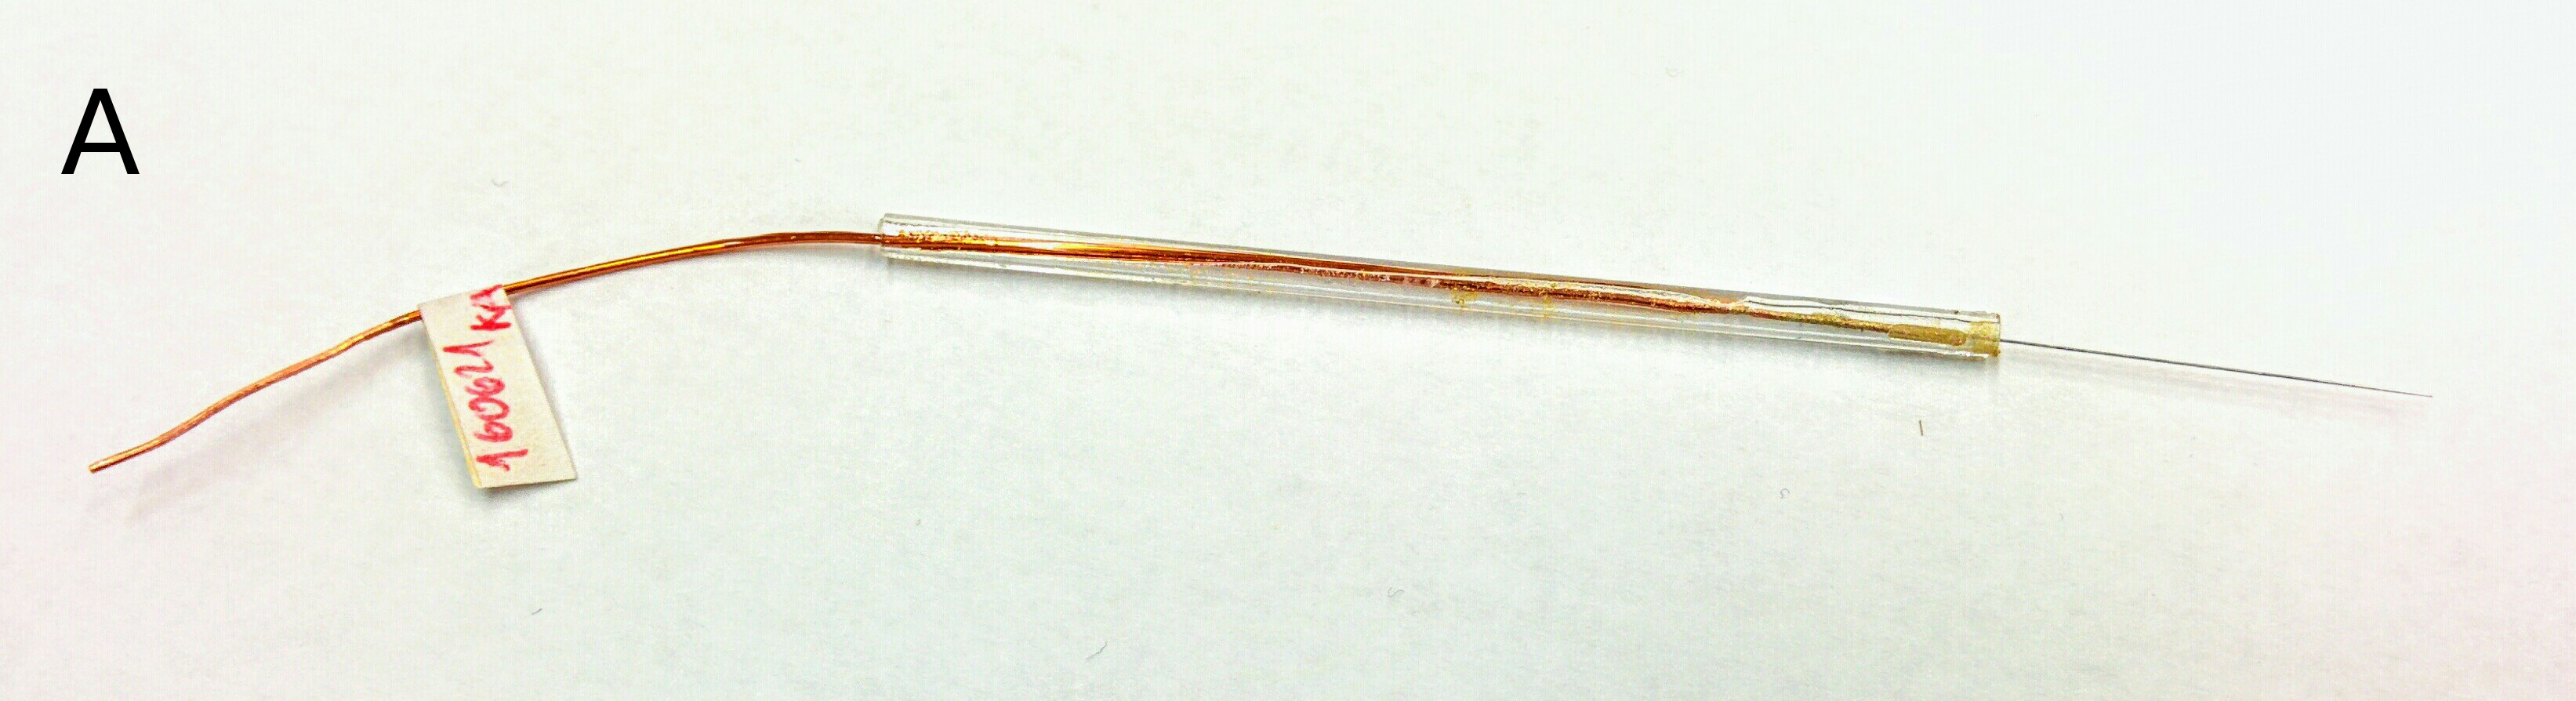
\includegraphics[width=0.6\textwidth]{img/sb_top.jpg}
%\caption[Antimony pH-sensitive microelectode.]{Antimony pH-sensitive microelectode.}
%\label{fig:sb_macro}
%\end{figure}
In this way, a continuous column of solid antimony was sealed into the glass tube.
Then, the glass tube with the antomony inside was melted again.
Since the melting points of antimony and borosilicate glass are very similar, they could be pulled together with standard glass blowing techniques, using tweezers.
With this method, very fine, glass-sealed antimony microwires can be obtained.
After this step, the diameter of the antimony wires was typically around 30 $\upmu$m.
If it was necessary, the microwires were pulled even further with a vertical puller (Sutter Instrument, 1 Digital Dr, Novato, CA 94949).
After the pulling stage, the wires were broken into pieces with a length of $3-4$ centimeters.
Then, they were investigated under an optical microscope to select pieces with a continuous antimony wire.
Due to the fragile nature of these microelectrodes, several of them were used through the course of my work.
The diameter of the antimony microelectrode used in a particular experiment is always specified in the discussion of that experiment.
To make electrical contact between the measuring instruments and the antimony microwires, a thin copper wire was glued to the glass shielding of antimony wire with conductive silver-epoxy (Amepox Microelectronics, Ltd.
90-268 Lodz Jaracza, Poland), making sure that the epoxy also covered the exposed antimony wire.
After curing for 1 hour at a temperature of 200 $\celsius$, the antimony microelectrodes were ready.
All electrodes were tested before usage by calibration in three buffer solutions (pH = 4, 7, 10). 



\paragraph{Antimony pH-sensitive combined macroelectrode}

Home-made antimony/silver combined macroelectrodes were used to study the effect of stirring on the delay in potentiometric measurements with antimony electrodes in general.
To make these electrodes, copper wires were soldered to one end of a $\sim$5$~$mm long silver and antimony wires ($d = 1~$mm).
Antimony wires with such diameter were made by sucking molten antimony into a $d_i = 1~$mm glass capillary.
Then, the glass was broken to aquire the antimony wire, which was then trimmed to $\sim 5~$mm length.
Both solder joints were strengthened mechanically by small segments of heatshrink tubes.
The obtained electrodes were carefully pushed down into a glass tube ($d_o = 5~$mm, $d_i=4~$mm) until they both reached the end of the glass tube.
Then, the remaining space in the tube was filled with epoxy resin.
Finally, after the resin was cured, the end plate was sanded down to 4000 grit, and polished on three different fiber cloths (Buehler), containing alumina slurry with decreasing particle size; 1$~\upmu$m, 0.3$~\upmu$m and finally 0.05$~\upmu$m.

\begin{figure}
\centering
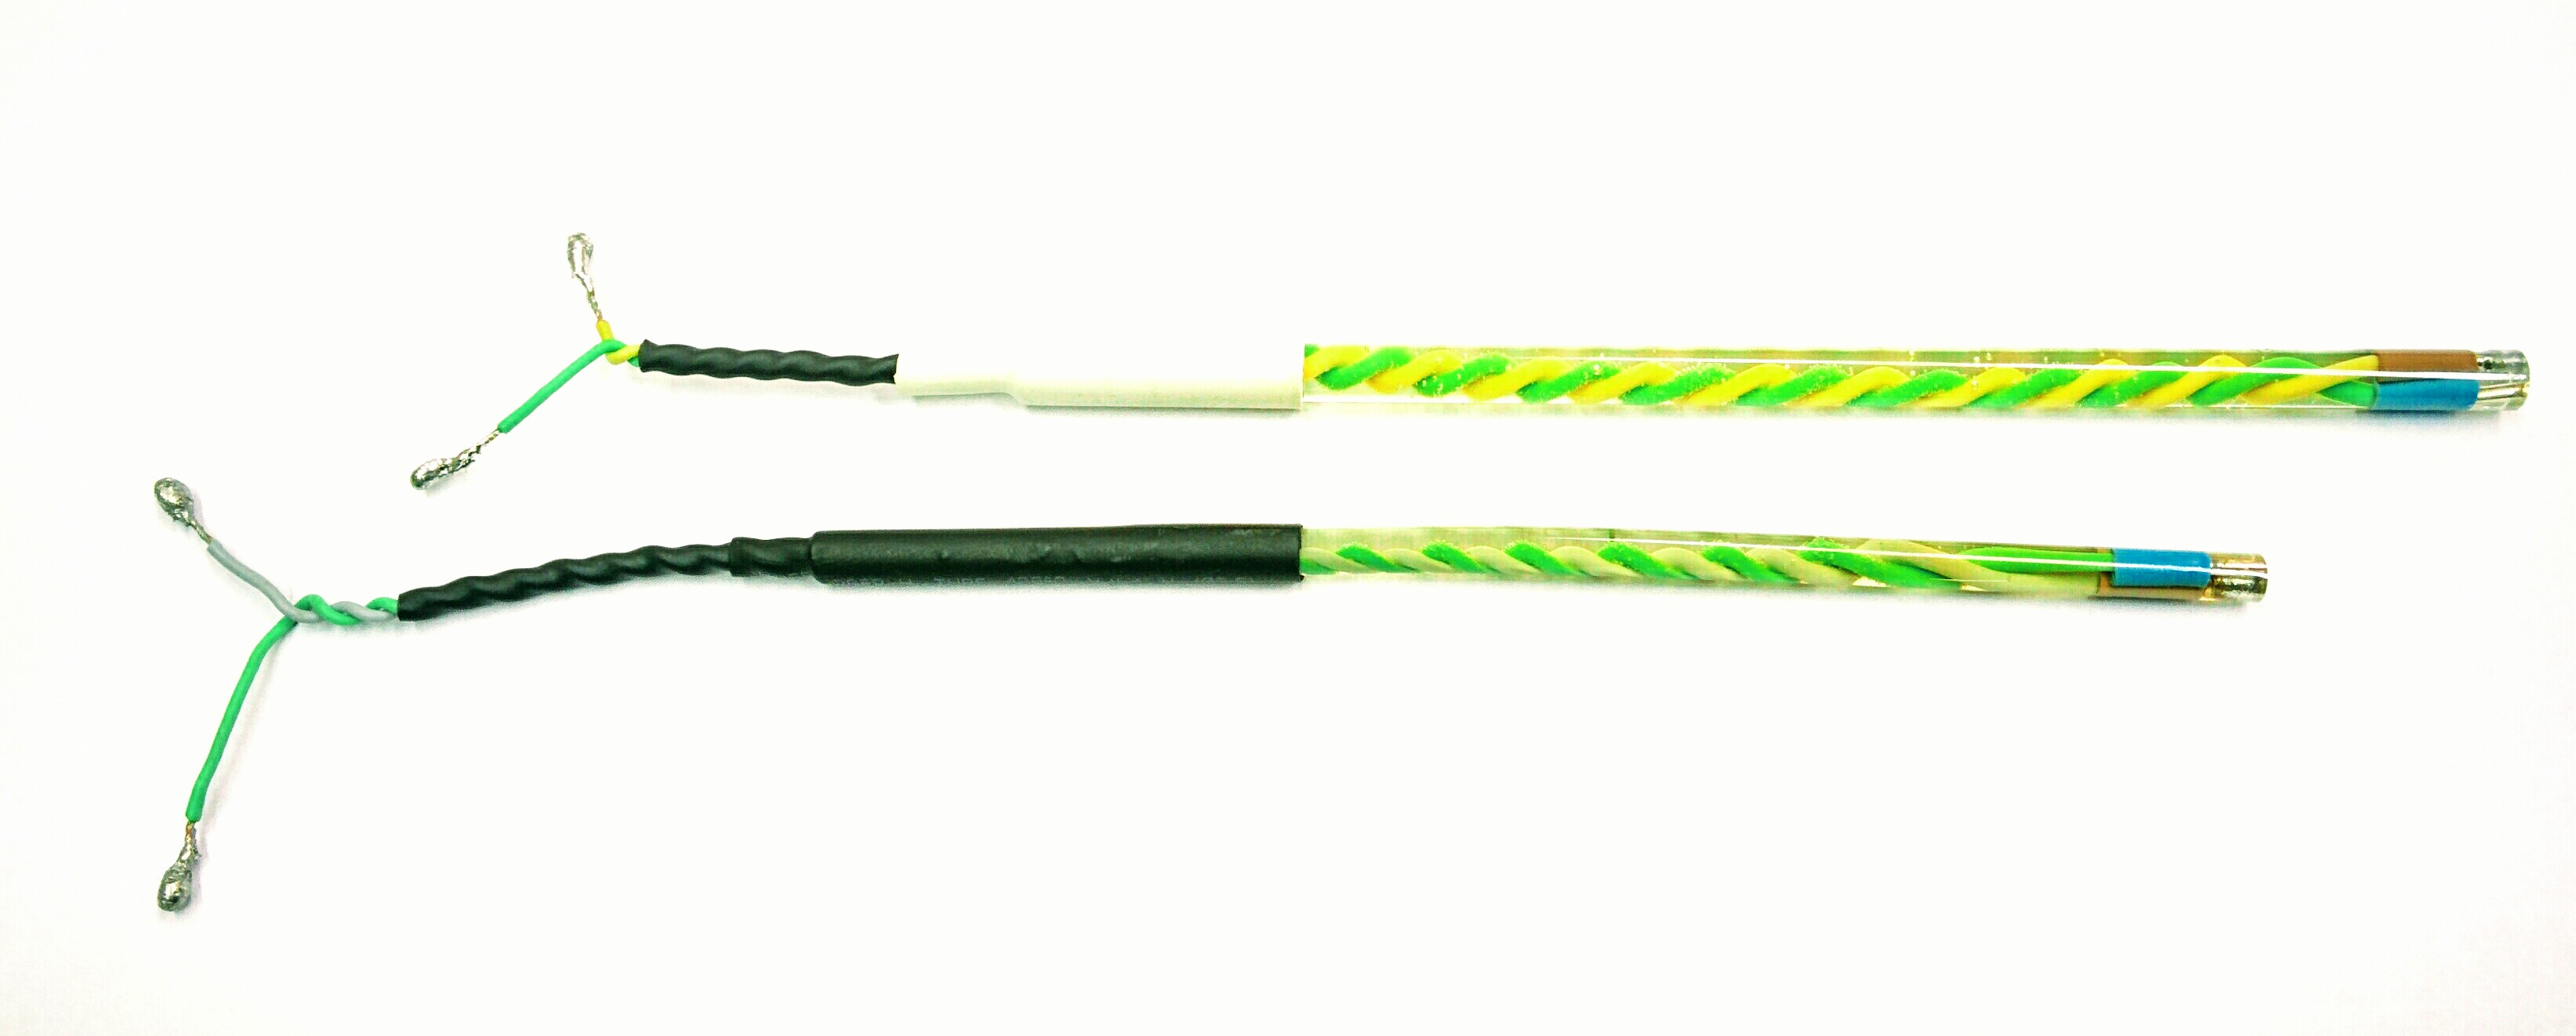
\includegraphics[width=0.693\textwidth]{img/sb_ag_top.jpg}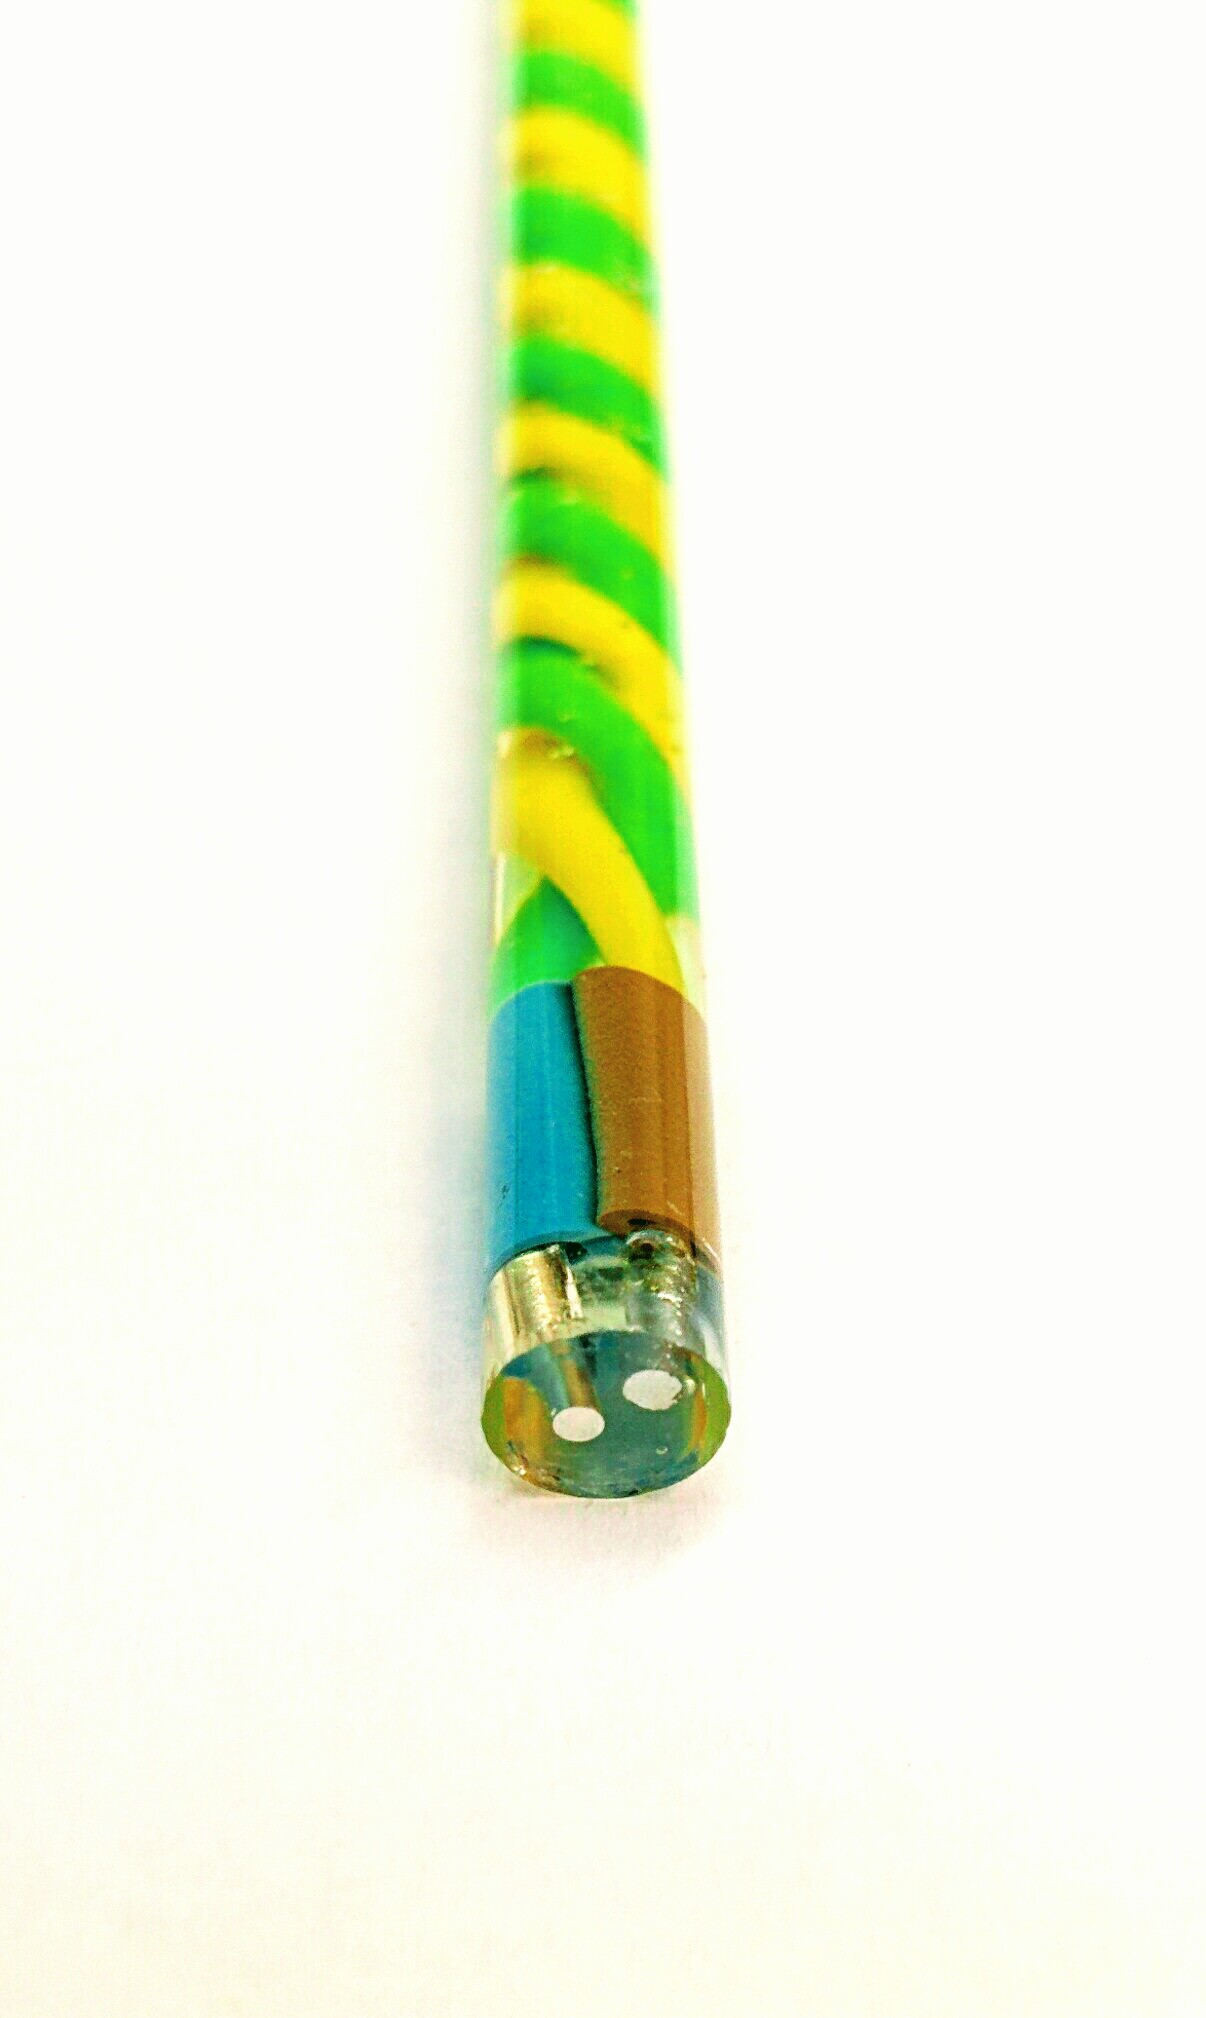
\includegraphics[width=0.165\textwidth]{img/sb_ag_front.jpg}
\caption[Home-made antimony/silver pH-sensitive combined macroelectrodes.]{Home-made antimony/silver pH-sensitive combined macroelectodes.
Left side: top view of two examples, right side: front view, displaying the antimony and silver electrodes. This type of electrode was used to investigate the effect of buffer stirring on response time.}
\label{fig:sb_macro}
\end{figure}

\paragraph{Tungsten pH-sensitive microelectrode}
Since tungsten has the highest melting point of all the elements (3422 $\celsius$), the method described in the previous paragraph cannot be used.
Instead, tungsten microwire with a diameter of 30 $\upmu$m (Element-explorer, Montreal, Canada) were sealed into a borosilicate glass capillary ($d_i$=1.12 mm, $d_o$=2 mm, no filament, World Precision Inc., Sarasota, Florida, USA).
To seal the microwire, one end of the capillary was closed with flame.
Then, a 1 cm long tungsten microwire was inserted from the other end, and pushed down to the sealed end.
The sealed end was melted again while vacuum was being applied from the open end.
The capillary was kept in the flame until 4-5 mm, about half of the microwire was sealed into the glass.
To make electrical contact between the microwire and the measuring instruments, a small piece of solder was inserted into the capillary.
The solder was melted in flame, and pushed down to the sealed end of the capillary.
While the solder was still melted, a copper wire was insterted into the solder.
Microelectrodes with 30 $\upmu$m tungsten filaments from a 100 W Tungsram incandescent lightbulb were also prepared, using the same method.
Fig. \ref{fig:tungsten_electrode} shows the tip of the finished tungsten microelectrodes.

\begin{figure}
\centering
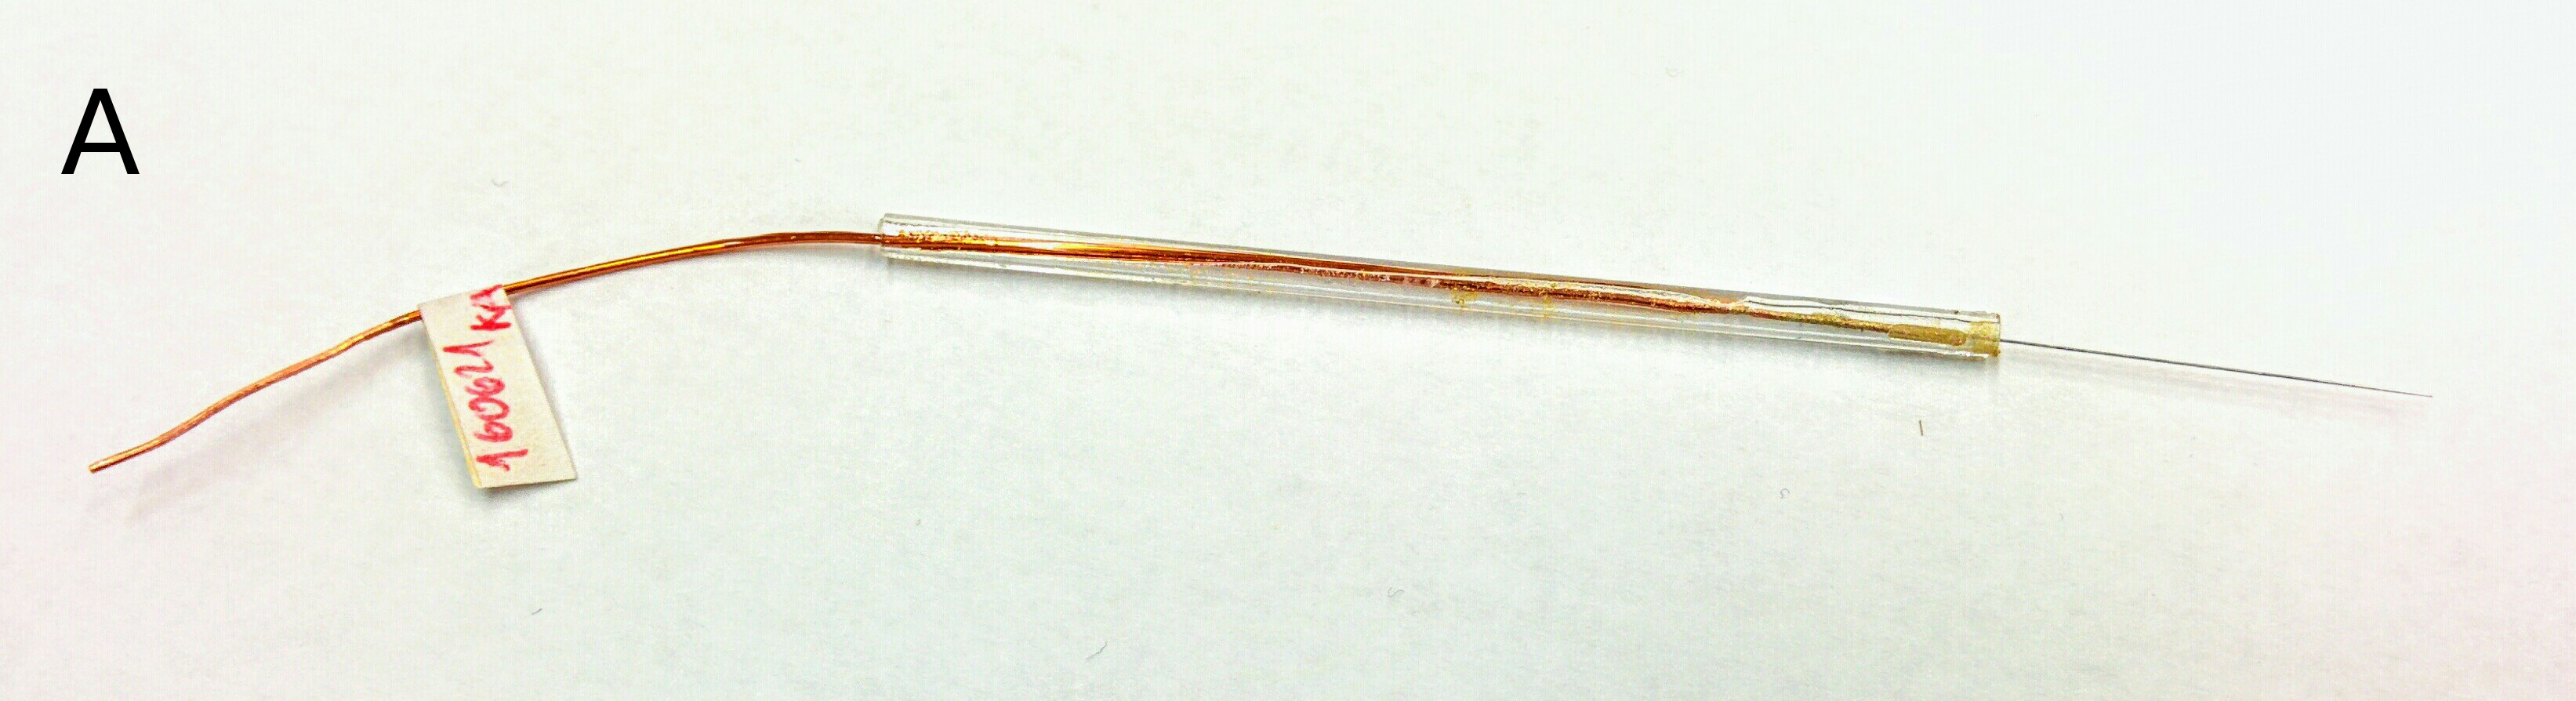
\includegraphics[width=0.9\textwidth]{img/sb_top.jpg}
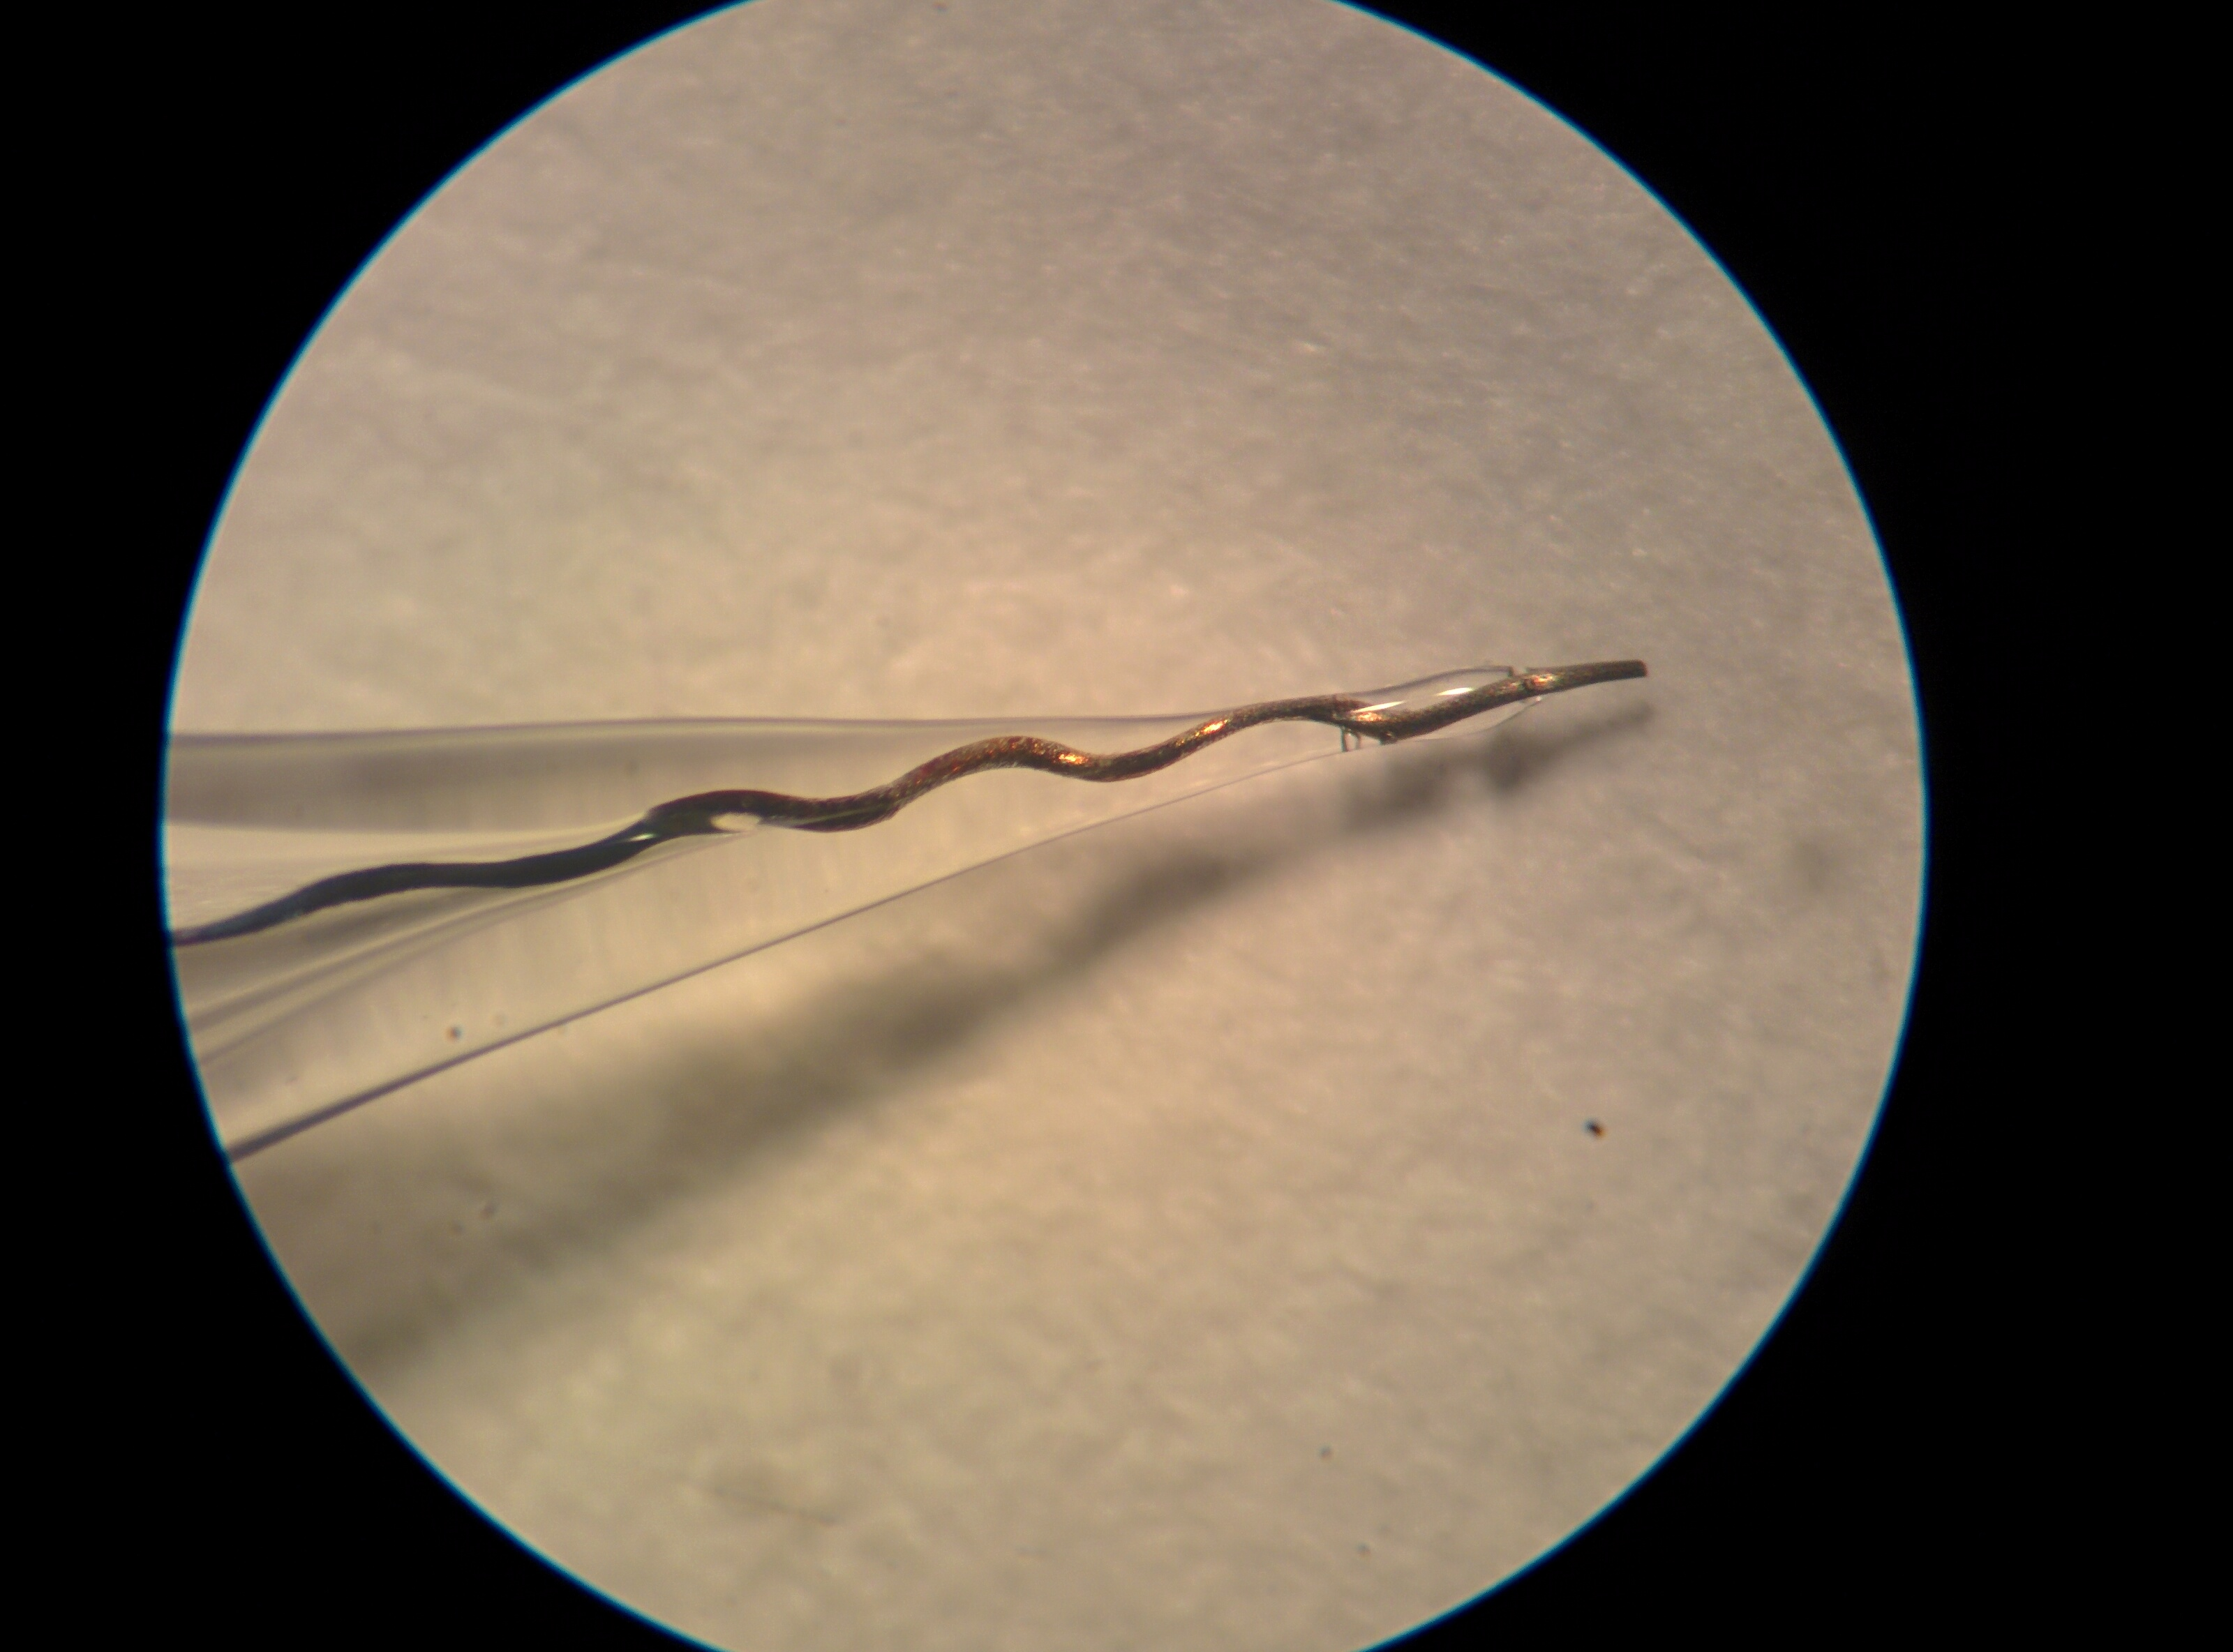
\includegraphics[width=0.45\textwidth]{img/wolfram_electrode1.jpg}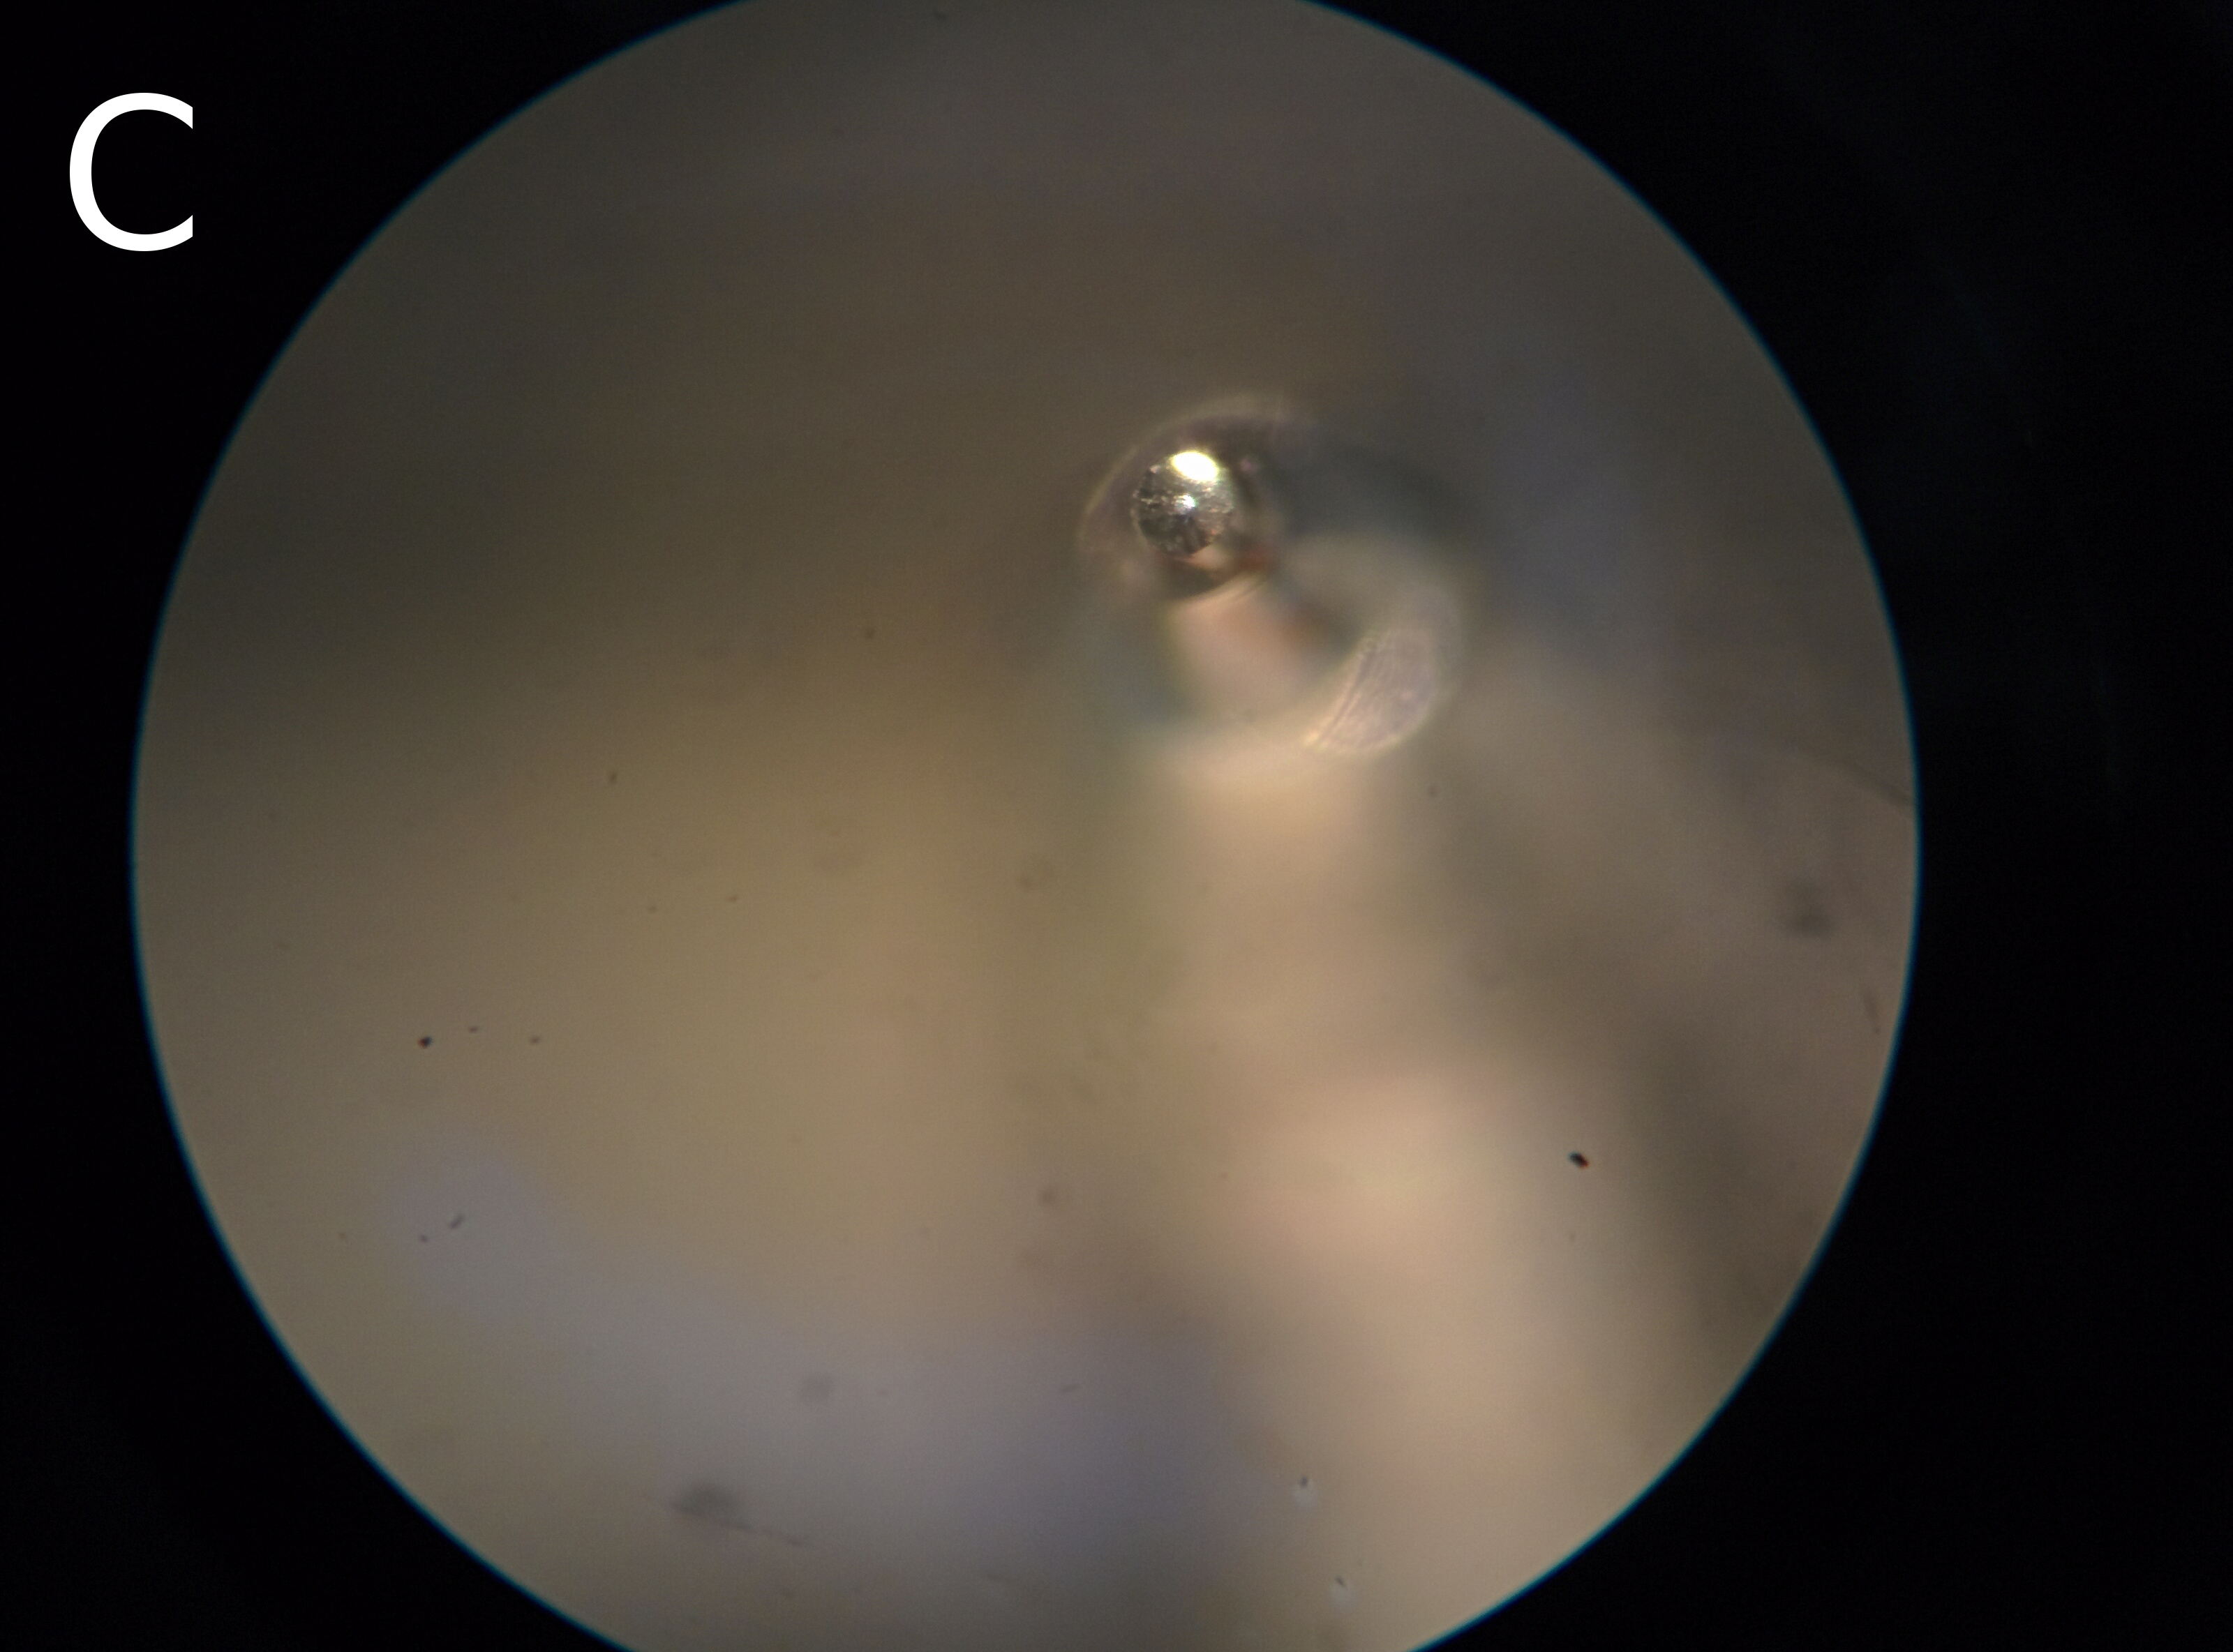
\includegraphics[width=0.45\textwidth]{img/wolfram_electrode2.jpg}

\caption[Antimony and tungsten microelectrodes for local pH measurements.]{Antimony and tungsten microelectrodes for local pH measurements.
Side view of the microelectrodes prepared from commercial 30 $\upmu$m tungsten microwires (C) and from 100 W Tungsram filaments (D).
Front view of the same electrodes (C and D).}
\label{fig:tungsten_electrode}
\end{figure}

	\subsubsection{Micropipette ion-selective electrodes}
Ion-selective microelectrodes were prepared using micropipettes pulled from bo\-ro\-si\-li\-cate glass capillaries B100-50-10 (Sutter, Novato, CA, USA).
The glass capillaries were first soaked in ,,piranha solution'', then thoroughly washed with twice deionized water and ethanol, and dried in oven at 105 \celsius.
Micropipettes were pulled from the capillaries by using a pipette puller (Sutter Instruments, type P-30, Novato, CA, USA).
The inner wall of the pipette tips were hydrophobized by exposing them to a solution of dimethyldichlorosilane in carbon tetrachloride through capillary action, and baking them at 200 $\celsius $ for 30 minutes in a closed petri dish.
The ionophore cocktail was filled into the micropipette tip under vacuum.
Two kinds of ionophores were used.
Bis-N,N-dicyclohexyl-malonamide and valinomycin for Mg$^{2+}$, and K$^+$, respectively.
Bis-N,N-dicyclohexyl-malonamide was synthesized at the Budapest University of Economics and Technology \cite{toth1993analytical}.
Selectivity coefficients of this ionophore toward Na$^+$ and H$^+$ ions are available in \cite{toth1993analytical}.
The composition of the ion-selective cocktail is given in Table \ref{table:cocktail}.
All the components in the ionophore cocktail were supplied by Sigma-Aldrich (St. Louis, MO), except the home-made ionophore.
The ionophore cocktail was cured for 24 hours, to allow the THF to be evaporated.
				
\begin{table}
                \caption[Composition of the mixture employed to produce the cocktail for the Mg$^{2+}$ and K$^+$ ion-selective microelectrodes.]{Composition of the mixture employed to produce the cocktail for the Mg$^{2+}$ and K$^+$ ion-selective microelectrodes.
Either bis-N,N-dicyclohexyl-malonamide or valimoycin was used.}
                \label{table:cocktail}
                \centering
                \begin{tabular}{r c c}
			& \multicolumn{2}{c}{Quantities for 200 $\upmu$L of the mixture}\\
			\cline{2-3}
                        Component & Content & wt\% \\
                        \hline
                        Tetrahydrofurane (THF) & 100 $\upmu$L & - \\
                        Poly(vynil chloride) (PVC) & 7.68 mg & 5.06 \\
                        bis-N,N-dicyclohexyl-malonamide & 2.23 mg & 1.47 \\
			valinomycin & 2.23 mg & 1.47 \\
                        Potassium tetrakis(4-chlorophenyl)-borate (PTCB) & 2.13 mg & 1.40 \\
			2-nitrophenyl octyl ether (oNPOE) & 139.79 mg & 92.07 \\
                \end{tabular}
\end{table}

				\paragraph{Liquid-contact ion-selective microelectrodes}
For the liquid contact version, an internal solution was backfilled with the assistance of a microsyringe.
The internal filling solution was 10 mM MgCl$_2$ and 0.25 M KCl in the case of a Mg$^{2+}$ ion-selective electrode, and 10 mM KCl for a K$^+$ ion-selective electrode.
The internal reference electrode for both liquid contact electrodes was a chlorinated silver wire.
To chlorinate silver wires, they were submerged into 1 M FeCl$_3$ solution for a few seconds, and cleaned from traces of Fe$^{3+}$ with cc. HCl.
The internal solution and the reference electrode were confined in the micropipette with hot glue.
A sketch and micrograph of the liquid-contact ion-selective microelectrode are shown in Fig. \ref{fig:solid_liquid}A.

\begin{figure}
\centering
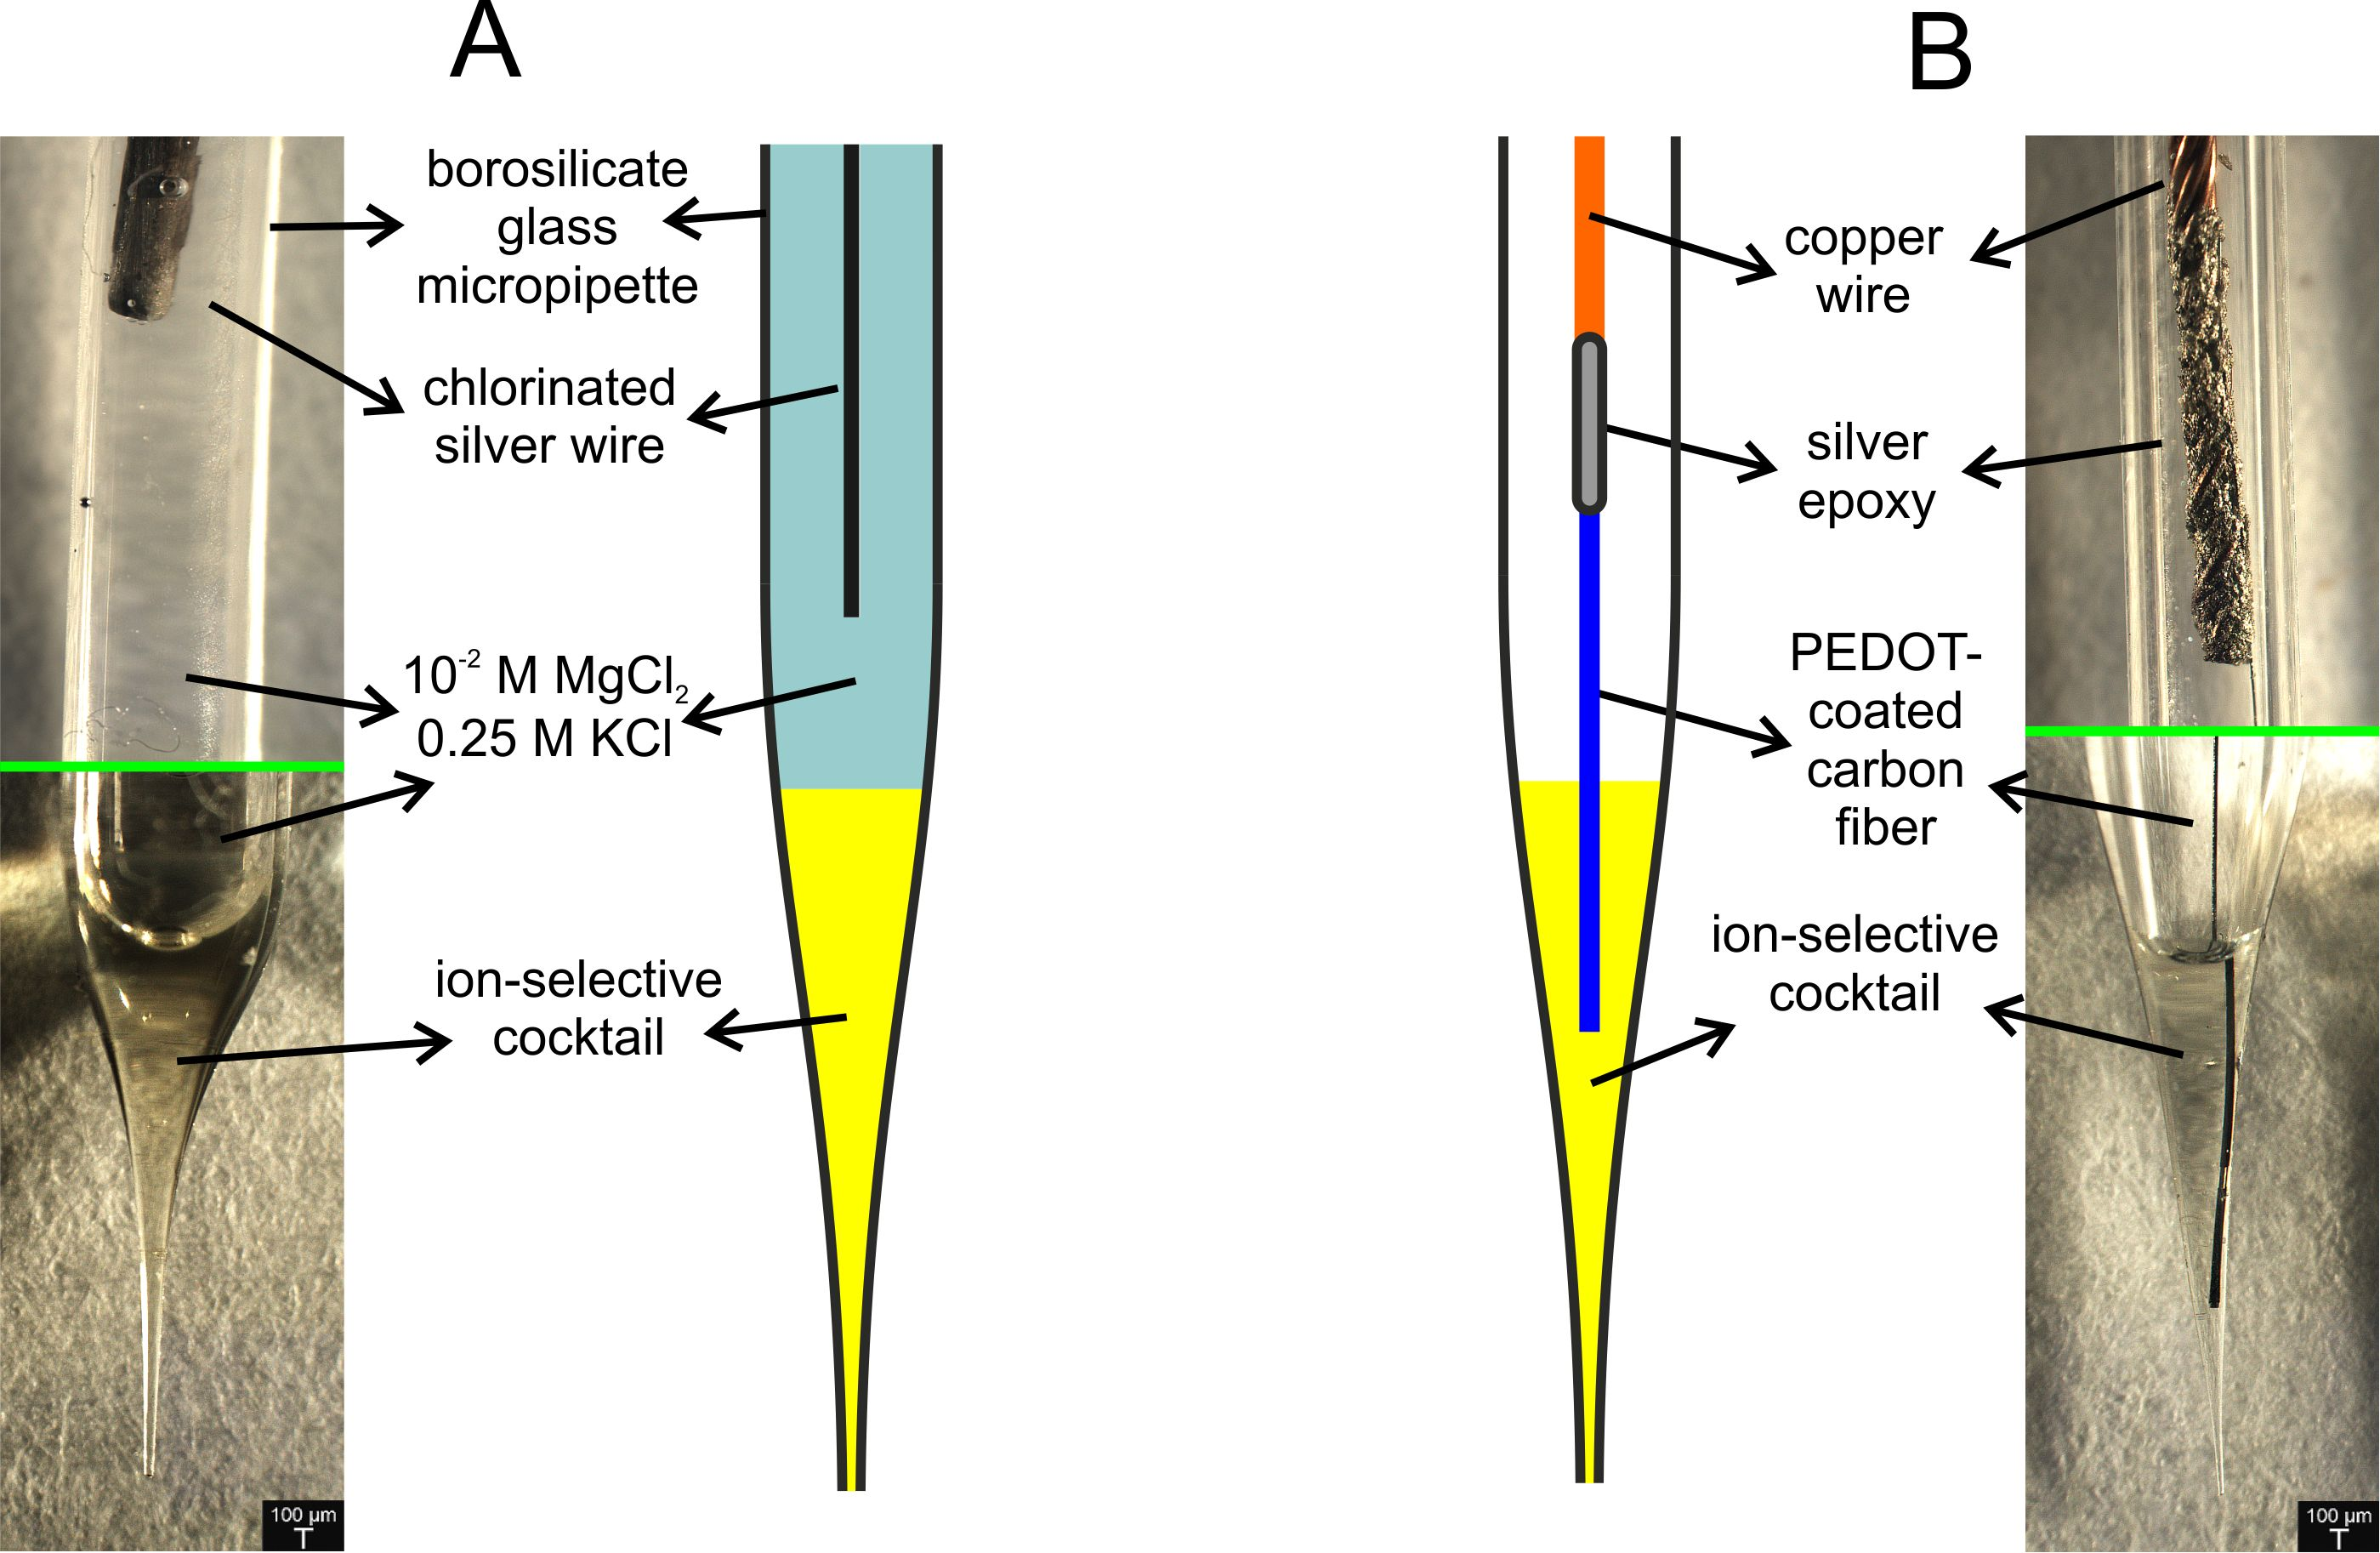
\includegraphics[width=0.8\textwidth]{img/liquid_solid.jpg}
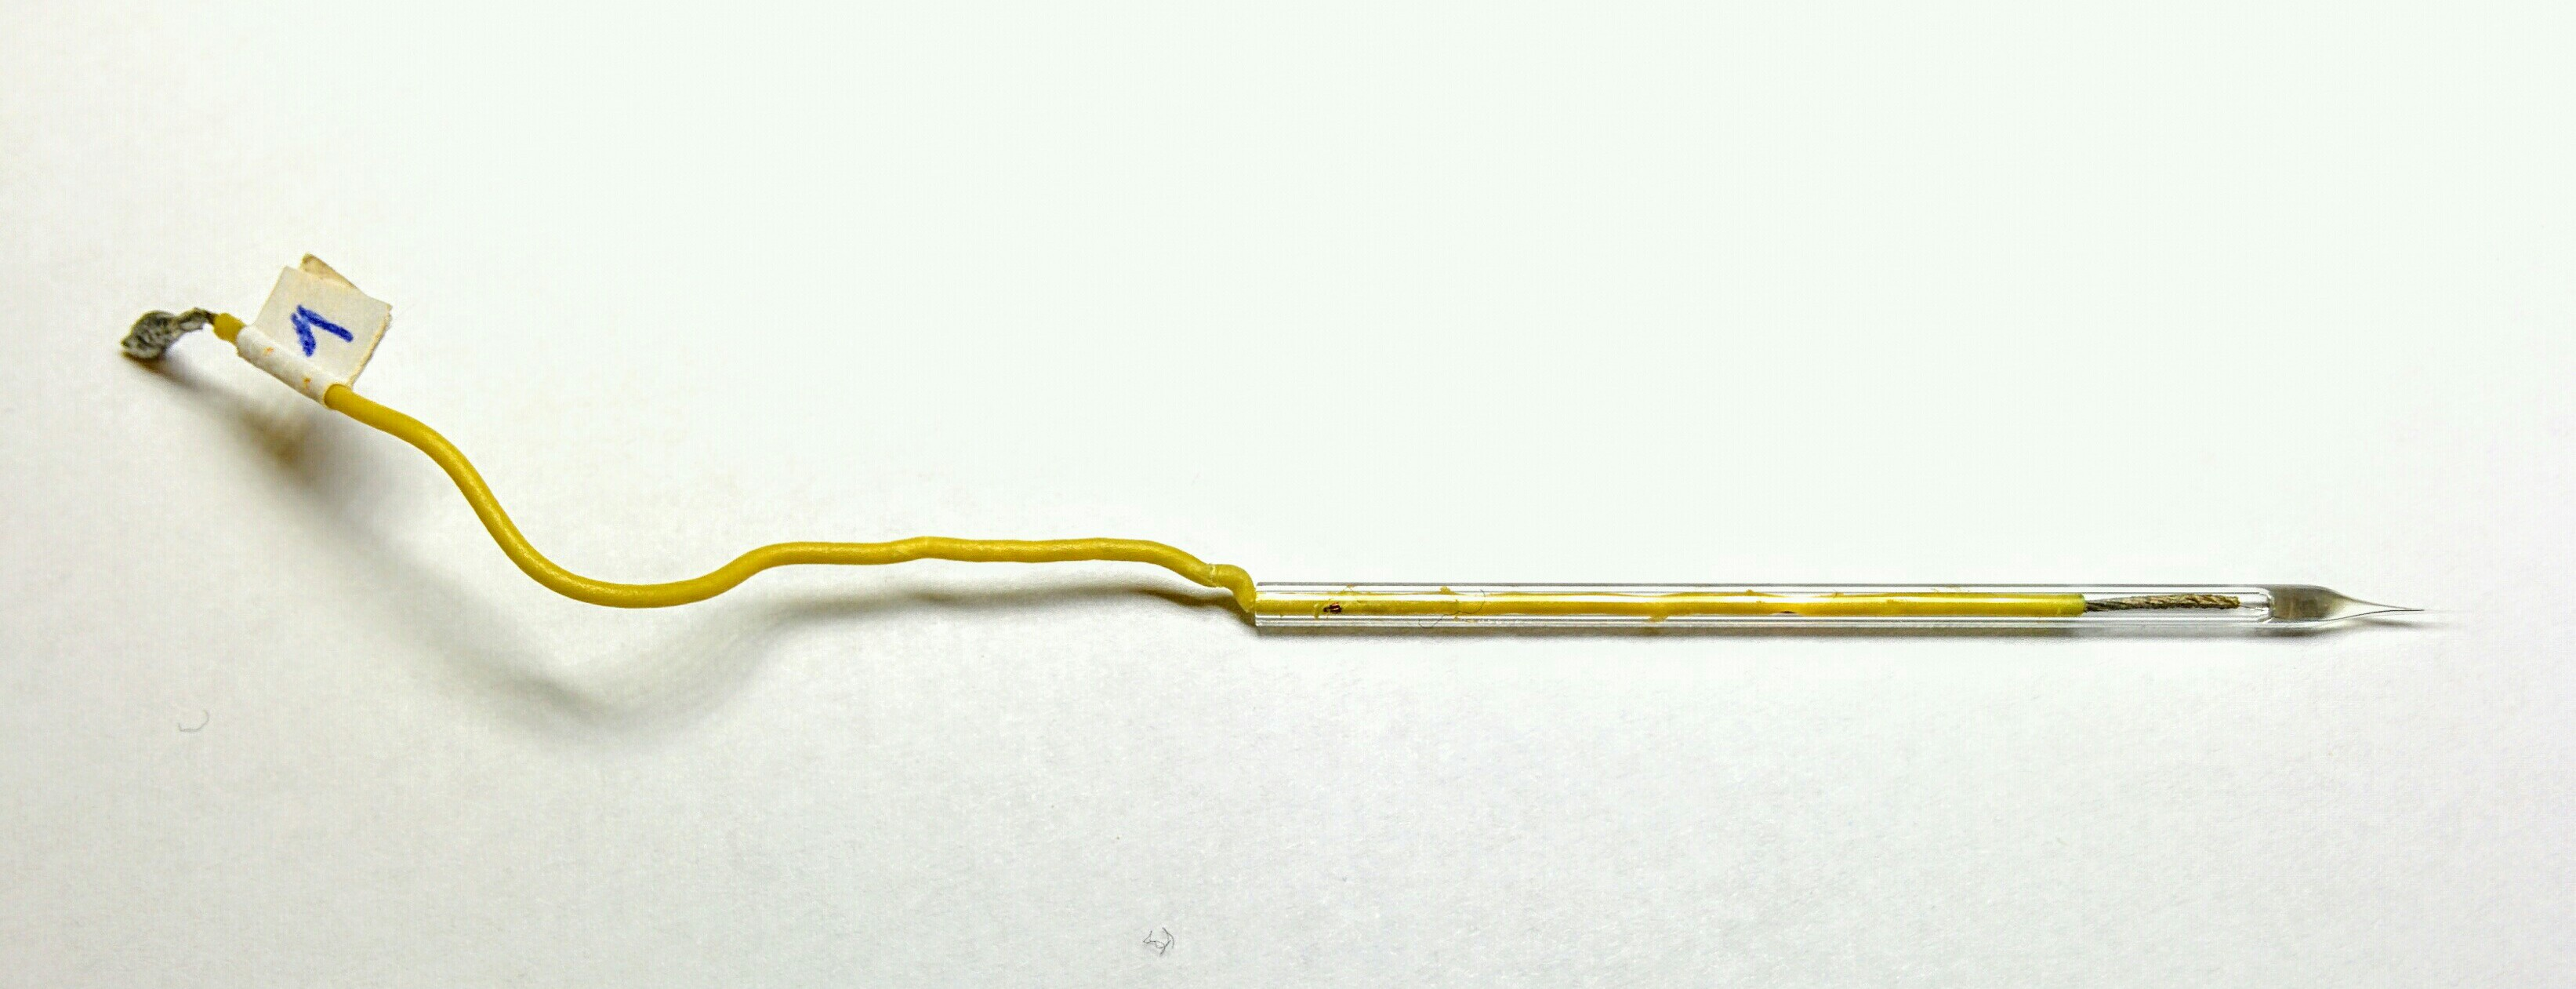
\includegraphics[width=0.8\textwidth]{img/mg_top.jpg}
\caption[Sketches and micrographs of the micropipette electrodes fabricated for the selective detection of Mg$^{2+}$ ions.]{Sketches and micrographs of the micropipette electrodes fabricated for the selective detection of Mg$^{2+}$ ions: (A) liquid-contact, and (B) solid-contact ISME's.
The K$^+$ solid contact micropipettes were identical in construction, except the composition of the ion-selecitve cocktail and the internal filling solution for the conventional electrodes, which was valinomycin, and $10^{-2}$ M KCl, respectively.}
\label{fig:solid_liquid}
\end{figure}

				\paragraph{Solid-contact ion-selective microelectrodes}
The solid-contact ion-selective microelectrodes were built using the same components employed for the fabrication of the conventional ISME, except in this case instead of the internal solution and chlorinated silver wire, the internal contact was provided by a PEDOT (poly(3,4-ethylenedioxythiophene)) coated 33 $\upmu$m diameter carbon fiber cut to 35 mm length.
The modified carbon fiber was pushed from the back opening of the pipette as close to the orifice as possible to minimize the thickness of the membrane between the solid contact and the sample, and therefore electrode resistance \cite{gyetvai2007solid}.
The top opening of the micropipette electrode was sealed using hot glue.
A micrograph of the resulting microelectrode is depicted in Fig. \ref{fig:solid_liquid}B.
				\paragraph{Preparation of the solid contact}
A copper wire was attached to the carbon fiber using silver-epoxy adhesive, to provide electrical contact.
The portion of the fiber to be in contact with the ionophore cocktail was then coated with PEDOT conductive polymer in an electrochemical cell composed of the carbon fiber as working electrode, an Ag/AgCl wire immersed in the electrolyte as quasi-reference electrode, and a platinum wire as the auxiliary electrode.
The monomer was 3,4-ethylenedioxythiophene dissolved in BMIM$^+$PF$_6^-$ (1-butyl-3-methylimidazolium hexafluorophosphate) ionic liquid \cite{gyetvai2007solid}.
Oxygen was purged from the EDOT-solution with nitrogen gas before and during the polymerization.
Then, PEDOT was polymerized with 10 consecutive cycles from -1.0 V to 1.5 V with a scanrate of 100 mV/s (Fig. \ref{fig:polymerization}).

\begin{figure}
\centering
\begin{tikzpicture}
\begin{axis}    [legend style={draw=none},
		legend pos=north west,
                xmin=-0.9,
                xmax=1.3,
                ymin=-0.00003,
                ymax=0.00006,
                width=10cm,
                height=9cm,
                xlabel={E, V},
                ylabel={i, A},
                clip marker paths=true]
\addplot [color=red, mark=none] table {data/edot/polymerization/cycl1.ocw};
\addplot [color=orange, mark=none] table {data/edot/polymerization/cycl2.ocw};
\addplot [color=yellow, mark=none] table {data/edot/polymerization/cycl3.ocw};
\addplot [color=green, mark=none] table {data/edot/polymerization/cycl4.ocw};
\addplot [color=cyan, mark=none] table {data/edot/polymerization/cycl5.ocw};
\addplot [color=blue, mark=none] table {data/edot/polymerization/cycl6.ocw};
\addplot [color=purple, mark=none] table {data/edot/polymerization/cycl7.ocw};
\addplot [color=black, mark=none] table {data/edot/polymerization/cycl8.ocw};
\addplot [color=red, mark=none] table {data/edot/polymerization/cycl9.ocw};
\addplot [color=orange, mark=none] table {data/edot/polymerization/cycl10.ocw};
\addlegendentry{1}
\addlegendentry{2}
\addlegendentry{3}
\addlegendentry{4}
\addlegendentry{5}
\addlegendentry{6}
\addlegendentry{7}
\addlegendentry{8}
\addlegendentry{9}
\addlegendentry{10}
\end{axis}
\end{tikzpicture}
\caption[Cyclic voltammetric electropolymerization of PEDOT onto the carbon fiber to create the solid internal contact for the ion-selective microelectrodes.]{Cyclic voltammetric electropolymerization of PEDOT onto the carbon fiber to create the solid internal contact for the ion-selective microelectrodes.
Top left inset indicates the order of the consecutive cycles.}
\label{fig:polymerization}
\end{figure}

\subsection{Instrumentation for the microelectrodes}
Microelectrodes have high resistance, therefore, to avoid loading error, some sort of impedance matching is necessary.
This is also crucial to minimize noise caused by stray capacitance.
Where the measuring apparatus lacked the high input impedance, a TL082 operational amplifier (Texas Instruments, Texas, USA) based unity gain voltage follower was used between the microelectrode and the measuring apparatus.
To record the potential difference between the measuring microelectrode and the reference electrode, either of these instruments were used:

\begin{itemize}
\item MeTeX Instruments M-3640D 3 1/2 Digit digital multimeter with the TL082 voltage follower,
\item Autolab Electrochemical Workstation (Metrohm, Herisau, Switzerland) with the TL082 voltage follower,
\item eDAQ Ecorder 402 Electrochemical Workstation with the eDAQ pH/ISE isoPod (eDAQ Pty Ltd, Australia),
\item eDAQ pH/ISE isoPod USB (eDAQ Pty Ltd, Australia),
\item Home made, Arduino based DAQ.
\end{itemize}

A 25 cm long shielded coaxial cable was used between the amplifier and the microelectrode.
Unshielded cable length was always minimized to less than a centimeter, excluding the length of the microelectrode itself.
Connection was always provided by BNC connectors.
The TL082 operational amplifier was powered by two 9V batteries, providing $\pm$9V, and a convenient ground node (Fig. \ref{fig:tl082}).

\begin{figure}
\centering
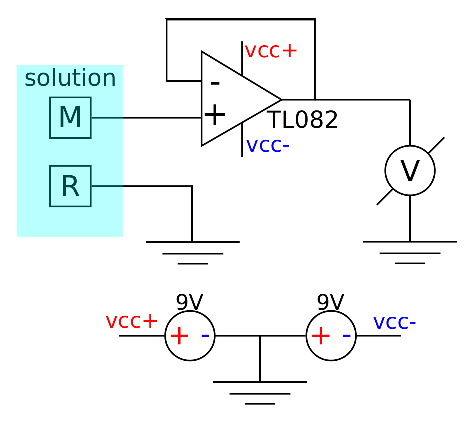
\includegraphics[width=0.5\textwidth]{img/circuit.eps}
\caption[The potentiometric cell with the TL082 voltage follower.]{The potentiometric cell with the TL082 voltage follower.
M: measuring electrode, R: reference electrode, V: voltage meter, $vcc+$ and $vcc-$: positive and negative rail of the power supply for the operational amplifier.} 
\label{fig:tl082}
\end{figure}

\subsubsection{Home-made, Arduino based DAQ}

The instrument is based on an DIP30 Arduino Nano, with an ATmega328 microcontroller (5V, 16MHz, Arduino AG, 2016, www.arduino.cc). A Texas Instruments ADS1115 16 bit analog-digital converter was connected to the microcontroller board through I$^2$C interface. A virtual ground between 0 and 5 V was established by a voltage divider circuit. The virtual ground was driven by an OPA342 low voltage, rail-to-rail, high input impedance operational amplifier, provided by Texas Instruments as a generous gift. The virtual ground was connected to the reference electrode, and one of the differential inputs of the AD1115. The measuring electrode was connected to the other differential input through a TI Tl082 high input impedance operational amplifier. The recommended supply voltage for this amplifier is $\pm 18~$V, but it worked surprisingly well with the $\pm 2.5~$V provided by the split 5 V of the USB port. The microcontroller ran the following program, a modified version of \cite{ads}: 

\begin{figure}
\centering
%\begin{circuitikz}[scale=1]\draw
% (0,0) node [ground] {} to [R, l=$R_1$, -*] (0,2)
% to [R, l=$R_2$, *-o] (0,4) 
% node [above] {5 V} (0,5)
% 
% (3,2.5) node [op amp] (opamp) {U1}
% (opamp.-) -| (1.5,4) to (4.5,4)
% (opamp.+) to (0,2)
% (opamp.out) to (4.5,2.5) to [*-] (4.5,4)
%
%;\end{circuitikz}
%
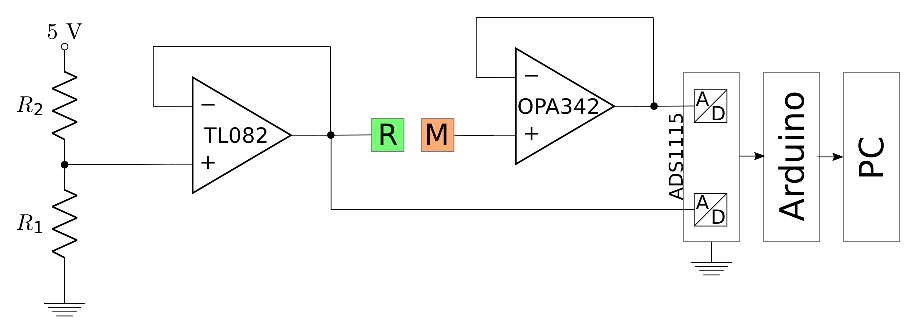
\includegraphics[width=1\textwidth]{img/arduino.eps}
\caption[Circuit diagram of the home-made Arduino-based DAQ.]{Circuit diagram of the home-made Arduino-based DAQ. [R] = reference electrode, [M] = measuring electrode. $R_1 = R_2 = 10~$k$\ohm$.}
\label{fig:daq_circuit}
\end{figure}

\begin{lstlisting}
#include <Wire.h>
#include <I2Cdev.h>
#include <ADS1115.h>

ADS1115 adc0(ADS1115_ADDRESS_ADDR_GND); 
float scalefactor = 0.03125;
float time;

uint16_t currentADCreadings;  

void setup(void)
{
  Serial.begin(115200);  
  Wire.begin();
  adc0.initialize();
  // initialize ADS1115 16 bit A/D chip
  adc0.showConfigRegister();
  adc0.setRate(ADS1115_RATE_860);
  // 860 samples/sec
  adc0.setMode(ADS1115_MODE_CONTINUOUS);
  // continuous sampling

  adc0.setGain(ADS1115_PGA_1P024);
  // 4x gain, +/- 1.024 V, 1 bit = 0.03125 mV, 2.4 MOhm
 
  adc0.setMultiplexer(ADS1115_MUX_P0_N1);
  // sets mux to differential
}

void loop(void)
{  
  time = 0.001 * millis();
  currentADCreadings=adc0.getConversion(); 
  Serial.print(time,4);
  Serial.print(' ');
  Serial.println(adc0.getMilliVolts(),4);
} 
\end{lstlisting}


\begin{figure}
\centering
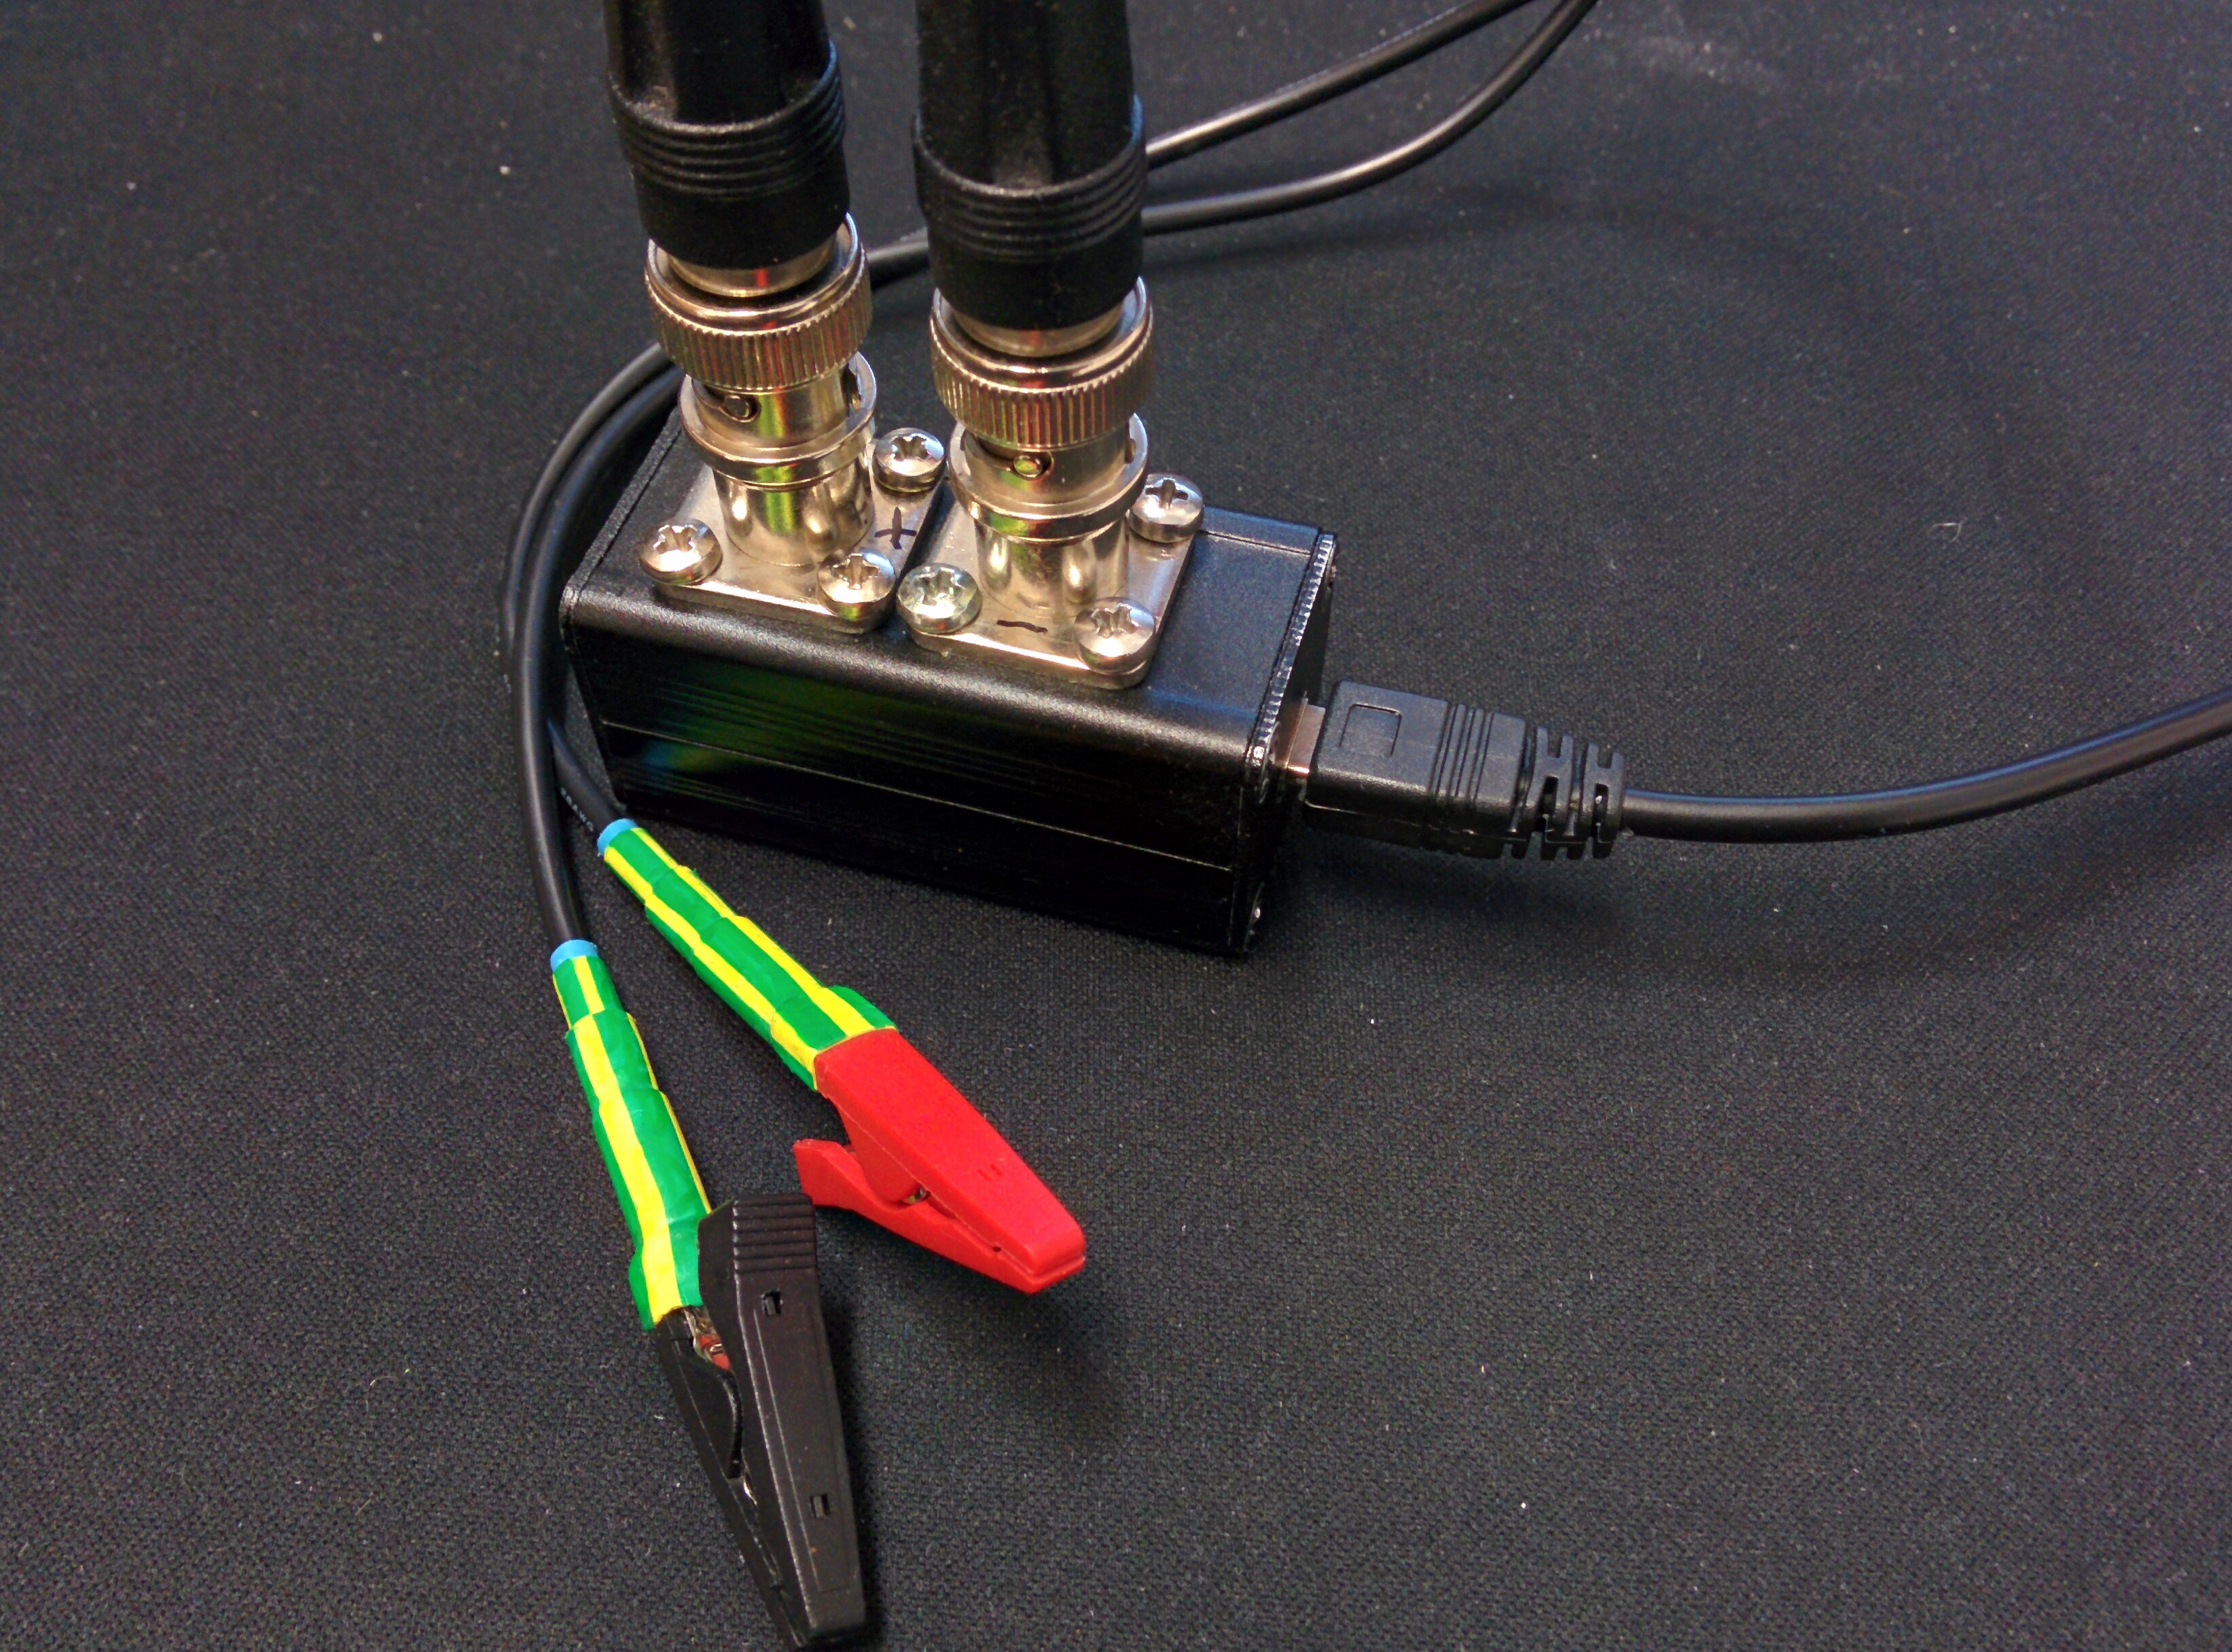
\includegraphics[width=0.4\textwidth]{img/daq1.jpg}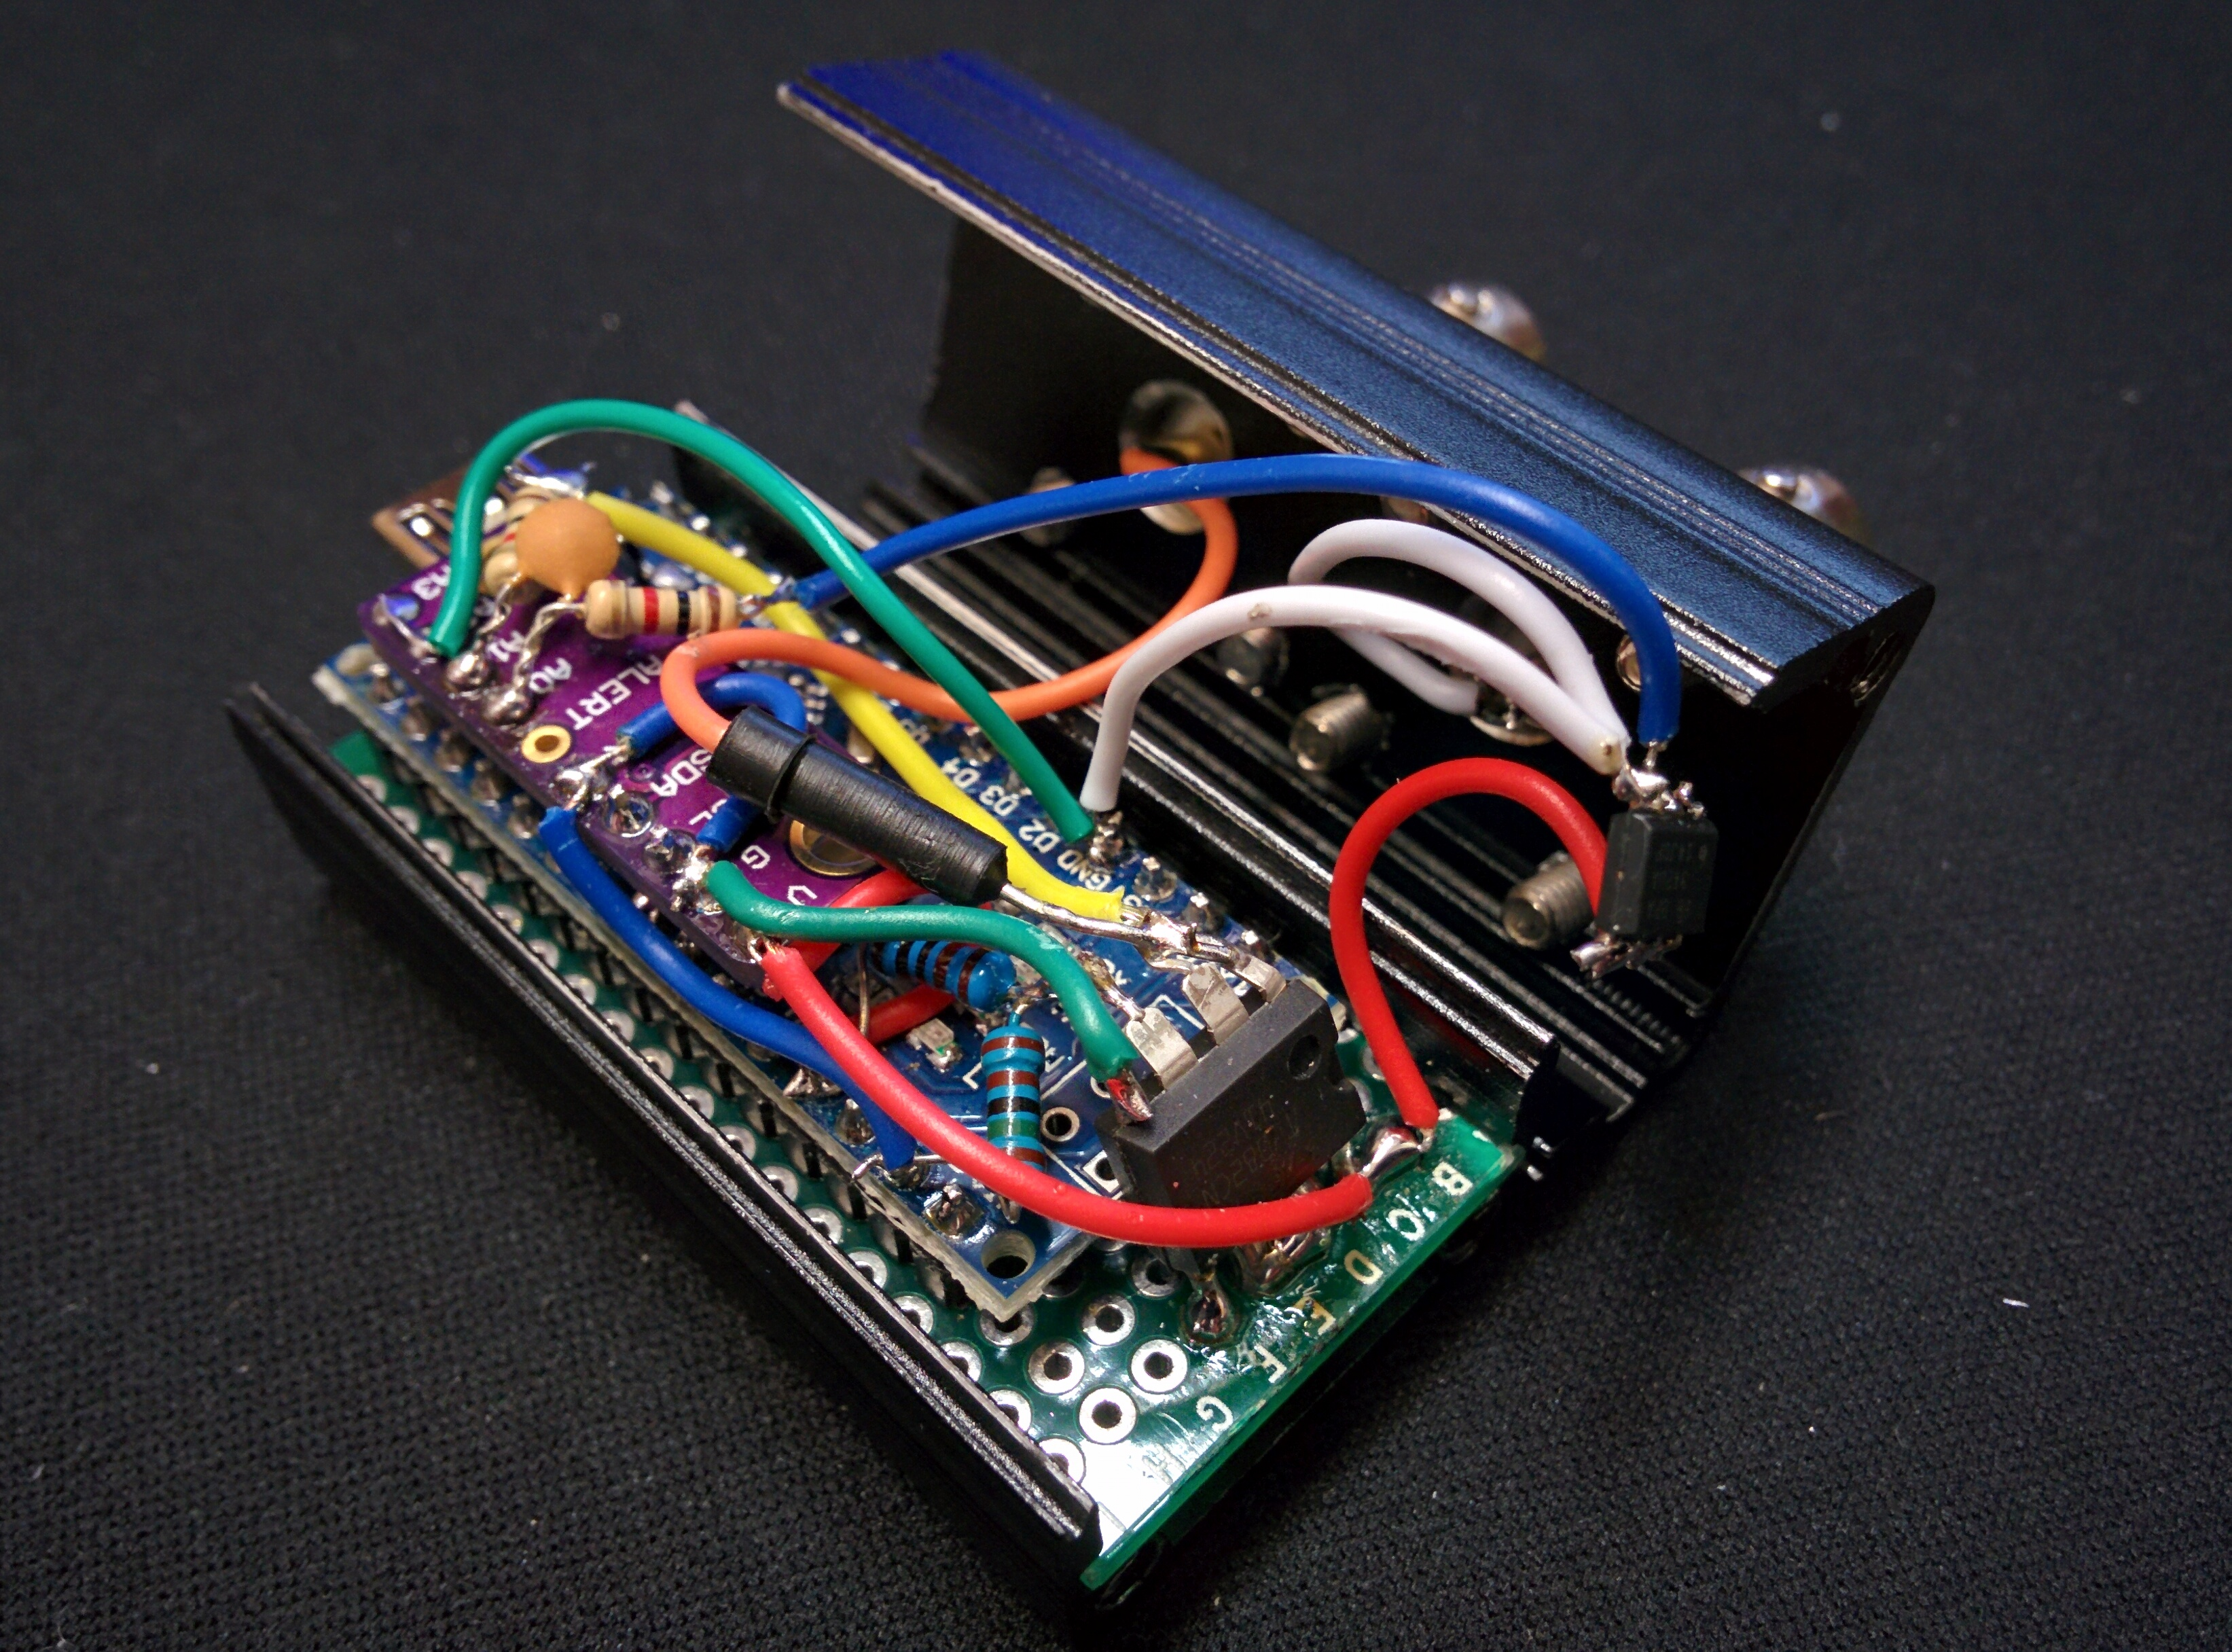
\includegraphics[width=0.4\textwidth]{img/daq2.jpg}
\caption[The home-made, Arduino based DAQ.]{The home-made, Arduino based DAQ.}
\label{fig:daq}
\end{figure}

While on the PC side (Debian Linux 9.x) the serial port was continuously monitored for incoming data, which was stored in the file $data.dat$:

\begin{lstlisting}
screen -d -m -S ads /dev/ttyUSB0 115200
screen -S ads -X logfile data.dat
screen -S ads -X log
\end{lstlisting}

The file was plotted live with the help of GNUPlot:

\begin{lstlisting}
#!/bin/sh
echo set grid
while true; do
 echo set yrange \[-1000:1000\]
 echo set xlabel \"time, s\"
 echo set ylabel \"E, mV\"
 echo plot \""<\(tail -n '-1000000' &&
	data.dat | sed -e '$ d' | &&
	sed -e '1 d'\)"\" &&
	with lines lc rgb \"red\" notitle
sleep 1
done
\end{lstlisting}

The GNU tools $sed$, and $tail$ was used to plot the last 1000000 data points only, ignoring the very last data point, which could potentially be incomplete at the time the plotting command is issued.

 		\subsection{Characterization of the microelectrodes}
			\subsubsection{Calibration}
For the micropipette ion-selective electrodes, calibration was performed in MgCl$_2$ and KCl dilution series, ranging from 10$^{-6}$ M to 10$^{-1}$ M.
The measuring and reference electrodes were submersed sequentially in each solution from lowest to highest concentration.
Potential was continuously measured against an Ag/AgCl/3M KCl reference electrode with a high input impedance eDAQ pH/ISE isoPod USB (eDAQ Pty Ltd, Australia).

Metal/metal-oxide microelectrodes were calibrated by measuring their potential in nine buffer solutions.
The typical calibration procedure was performed by introducing the microelectrode in a sequence of buffer solutions initiated with the most alkaline solution.
In this way, the tip was exposed to solutions of increasing acidity.
 
			\subsubsection{Internal resistance}
The voltage divider method was used to measure the resistance of the microelectrodes using 1 mM MgCl$_2$ + 1 mM NaCl solution.
The electrochemical cell consisted of an Ag/AgCl/3M KCl reference electrode and a freshly prepared microelectrode.
The measuring electrode was connected to the voltage follower as shown in Fig. \ref{fig:divider}.
After a steady reading was achieved, a precision resistor $R$ was interconnected between the inputs of the voltage follower.
The experiment was performed with two different precision resistors, namely 0.5 and 1.0 G$\ohm$

\begin{figure}
\centering
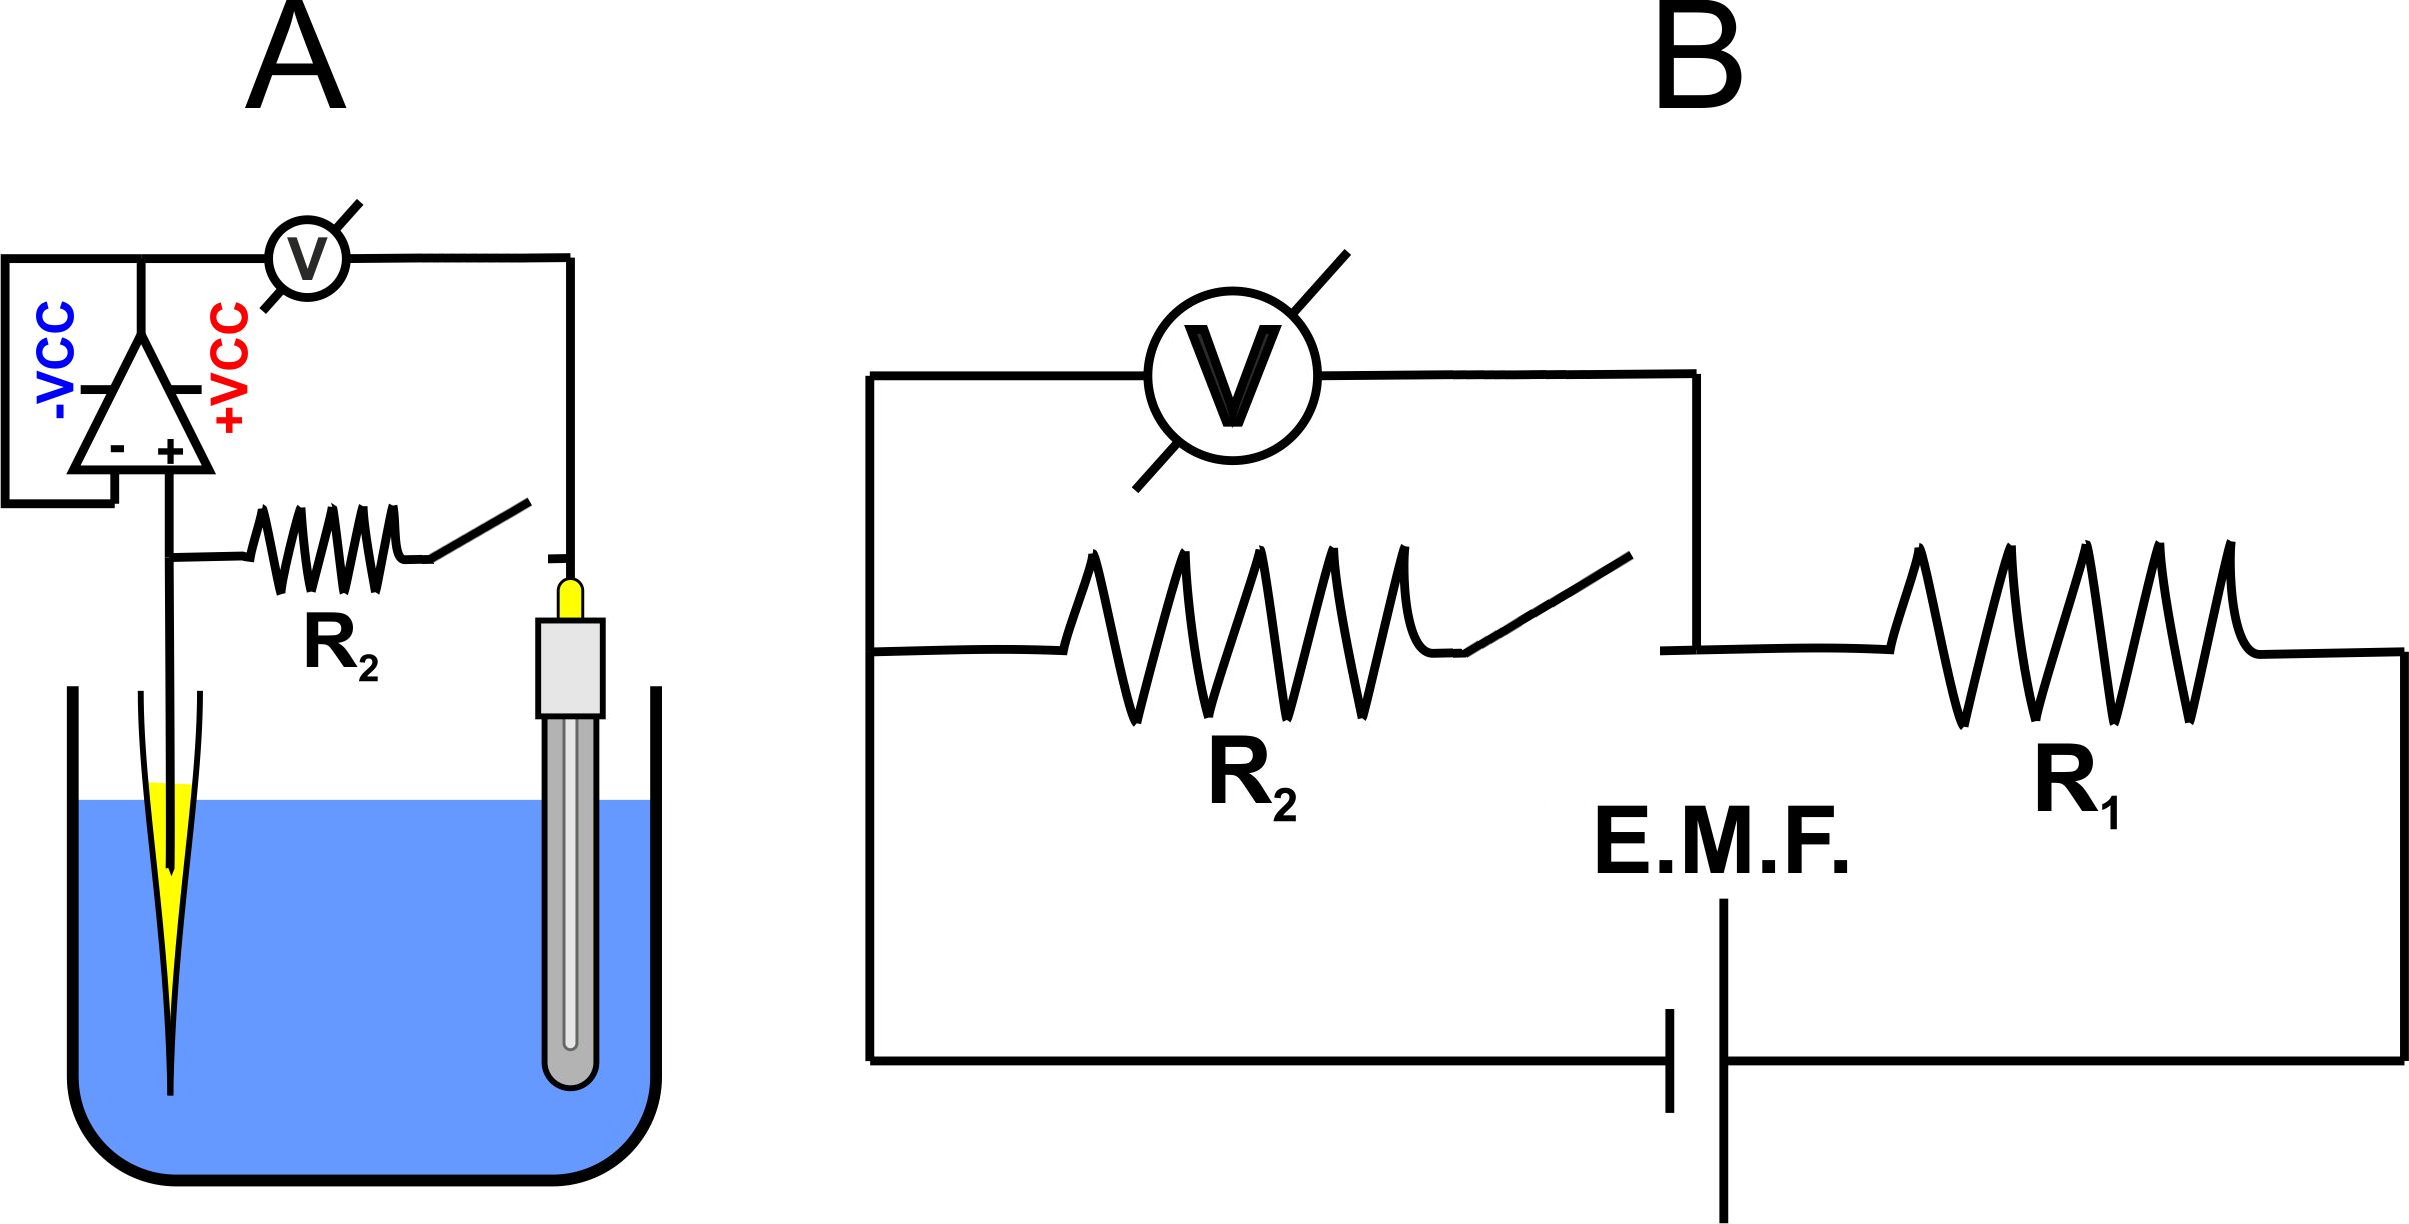
\includegraphics[width=0.7\textwidth]{img/divider_switch.jpg}
\caption[Voltage divider circuit to measure electrode resistance]{Voltage divider circuit to measure electrode resistance.
The connection between the measuring and the reference electrodes through $R_2$ could be turned on and off with a switch.} 
\label{fig:divider}
\end{figure}

The resistance of the antimony microelectrodes were also measured directly by attaching one probe of a high precision multimeter to the microelectrode, while submersing the other probe and the tip of the microelectrode into a beaker containing mercury.

			\subsubsection{Response time}
The response time of the microelectrodes was measured by recording the response to a sudden change in ion activity. The method is based on a modified version of the dual drop cell method \cite{lamaka2009novel}, called the \emph{,,hanging drop method''}.
The tip of the measuring electrode was positioned in the close vicinity of the ceramic frit of the reference electrode. Both electrodes are in contact with the same drop of solution, that is hanging from the reference electrode. This arrangement is depicted in Fig. \ref{fig:hanging}.

\begin{figure}
\centering
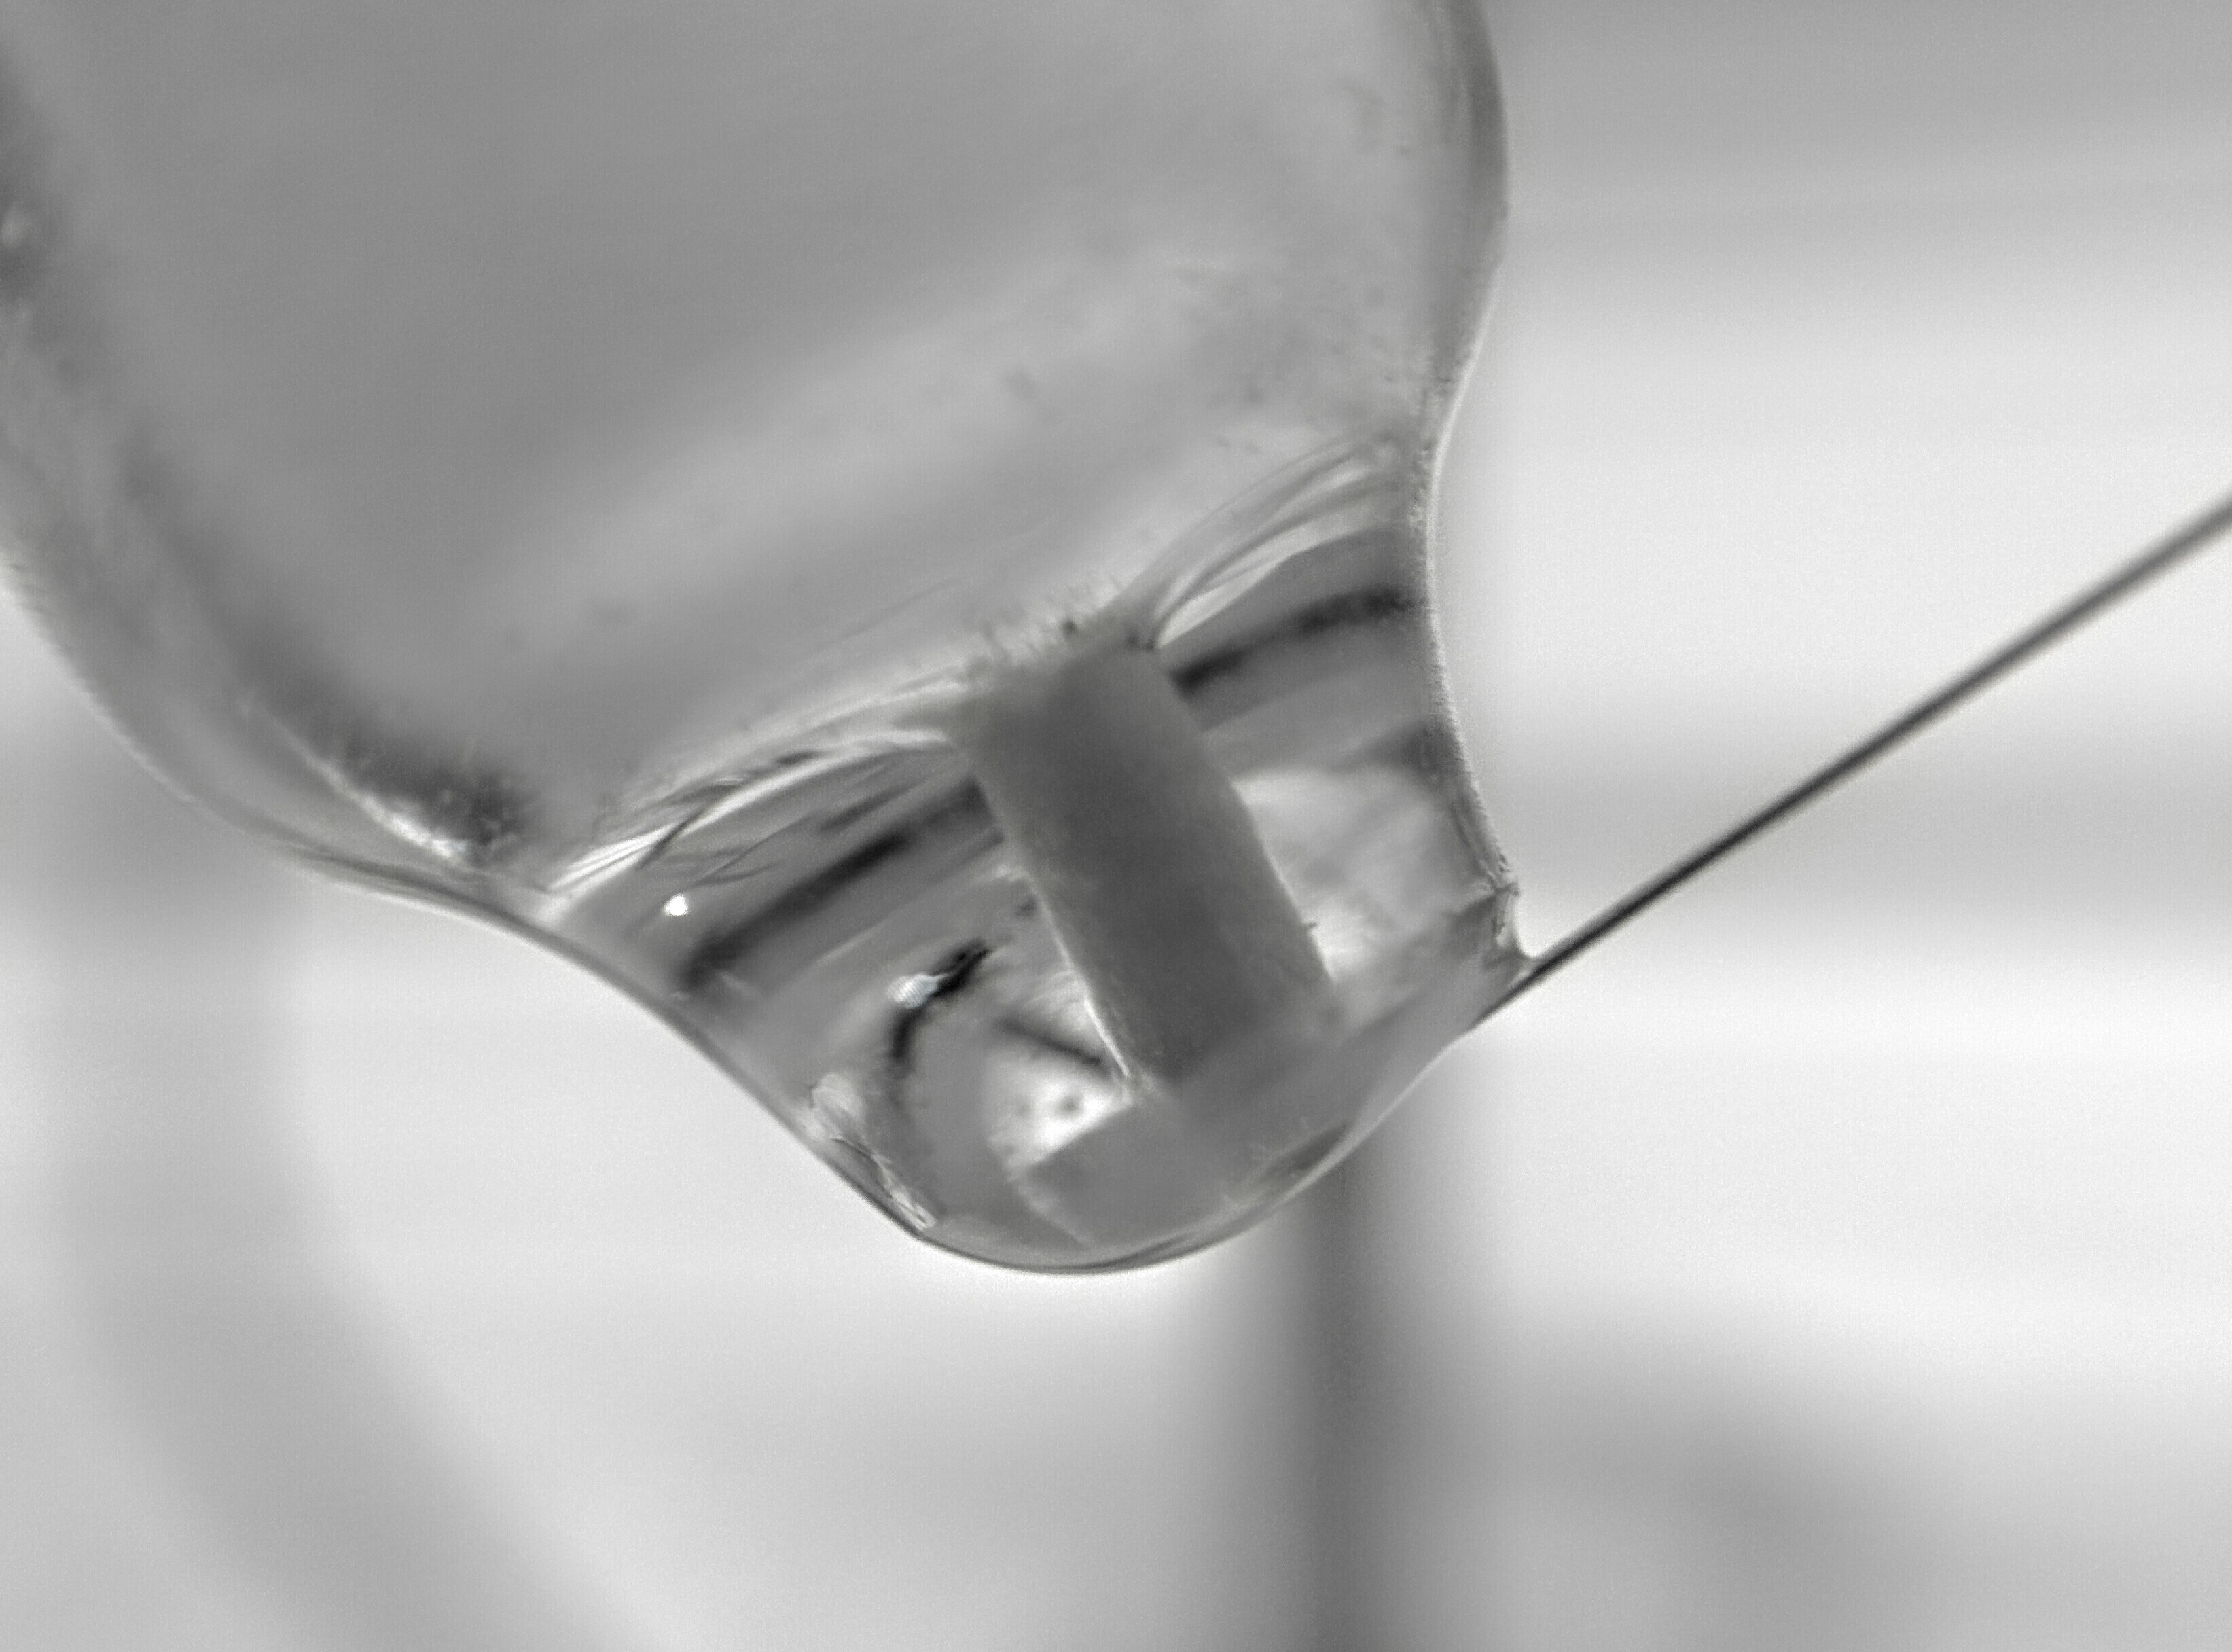
\includegraphics[width=0.6\textwidth]{img/hanging.jpg}
\caption[The hanging drop method]{The hanging drop method to measure response time.
The tip of the measuring electrode is touching the ceramic frit of the reference electrode. They are both in contact with a small drop of solution that is hanging from the reference electrode. In this way, the potentiometric cell is intact even while the solution is being exchanged, and a sudden activity step can also be realized.} 
\label{fig:hanging}
\end{figure}

When the equilibrium potential was reached, the first solution was removed, and the surface of the second solution was slowly approached to the drop of the first solution hanging from the reference electrode, with the help of a laboratory stand with an adjustable height. When the surface of the second solution reached the drop of the previous solution, a sudden jump in ion activity was realized, corresponding to the difference between the ion activities between the first, and the second solution. This method was employed in the response characterization of the antimony microelectrodes.

To characterize the Mg$^{2+}$ ion selective electrodes, they were immersed in a solution of 0.1 M MgCl$_2$ + 1 mM NaCl and then moved to the second solution of 0.01 M MgCl$_2$ + 1 mM NaCl after a stable potential was reached in about 3 minutes.
The time needed to reach 95\% of the total potential change caused by the change in Mg$^{2+}$ ion concentration was regarded as response time $\uptau_{95}$ (Fig. \ref{fig:response_time_explained}).

\begin{figure}
\centering
\begin{tikzpicture}
\begin{axis}    [
                only marks,
                xmin=-100,
                xmax=150,
                ymin=-130,
                ymax=-70,
                width=9cm,
                height=7cm,
                xlabel={time, s},
                ylabel={E vs. Ag/AgCl/3 M KCl, mV},
                /pgf/number format/.cd, use comma, 1000 sep={}
                ]
                \addplot 	[mark=*, 
				mark size=0.5,
				x filter/.code={\pgfmathparse{\pgfmathresult-1017}},
				%y filter/.code={\pgfmathparse{\pgfmathresult-10}}
				]
				table {data/electrodes/solid_response_time.txt};
		\draw (axis cs:-100,-87) -- (axis cs:50,-87) node[right] {E$_0$};
		\draw (axis cs:-70,-115.5) node[above] {E$_{95}$} -- (axis cs:33,-115.5);
		\draw (axis cs:-70,-116.4) node[below] {E$_{\infty}$} -- (axis cs:1183,-116.4);
		\draw[{latex[scale=5.0]}-{latex[scale=5.0]}] (axis cs:-42,-87) -- (axis cs:-42,-116.4);
		\draw (axis cs:33,-82) node[above] {$\tau_{95}$} -- (axis cs:33,-130);
		\draw (axis cs:0,-82) node[above] {$\tau_{0}$} -- (axis cs:0,-130);
		\draw (axis cs:-45,-101.7) node[left] {$\Delta$E};
\end{axis}
\end{tikzpicture}
\caption[Illustration of the parameters used for the determination of response time.]{Illustration of the quantities used for the determination of response time.
$E_0$: electrode potential prior to change in the activity (of the measured ion), $E_{eq}$: equilibrium electrode potential after the change in activity.
$\Delta E$: total difference between $E_{eq}$ and $E_{eq}$, $E_{95}$: electrode potential when 95\% of the total change has occured.
$\tau_0$: time instance when the change occurs, $\tau_{95}$: time instance when $E_{95}$ is reached.
$\Delta \tau_{95}$: difference between $\tau_{95}$ and $\tau_0$.}
\label{fig:response_time_explained}
\end{figure}

			\subsubsection{RC time constant}
$RC$ time constant was determined with two different methods.
For the antimony and tungsten pH-electrodes, $RC$ time constant was measured directly from the response curve using the activity step method.
The transient response curve of the potentiometric cell was recorded while the buffer was changed from pH 6 to pH 4, then Eq. \ref{eq:rc} was fitted on the curve.
In the fitted function, $RC$ is the only variable parameter, and can be directly obtained.

For the micropipette electrodes, a different method was used.
Resistance and capacitance of the potenciometric circuit was measured individually.
Resistance of the measuring electrode was determined with the voltage divider method described in the previous section.
In this case however, an $R$ = 50 M$\ohm$ 1\% precision resistor was inserted between the measuring and reference electrodes, then the cell potential difference was continuously measured in 10$^{-2}$ M MgCl$_2$ solution.
After arriving at equilibrium potential difference, the resistor was removed, and the measurement was continued until a new equilibrium signal was reached.
Electrode resistance can be calculated with the formula

\begin{equation}
\label{eq:divider}
        R_{ISME}
        =
        R
        \frac
                {E_{OCP} - U_{R}}
                {U_{R}}
\end{equation}
where R$_{ISME}$ is the resistance of the ion-selective microelectrode, $R$ is 50 M$\ohm$, $E_{OCP}$ is the open circuit potential difference, and $U_{R}$ is the potential difference between the electrodes while the resistor is introduced in the circuit.

The capacitance of the circuit is mainly due to the capacitance of the input amplifier, and the capacitance of the cable leading from the electrodes to the amplifier input.
The capacitance of the amplifier input was measured by applying a low impedance -1.5 V step between the inputs of the amplifier through a 50 M$\ohm$ resistor, and the time necessary to reach 63\% of the total change in potential difference ($\tau$ = $R\times C$) was measured.
Then, the input capacitance could be calculated with the $C = \tau/50$ M$\ohm$ formula.
		
	\section{SECM targets}
With the exception of the micropipette ion source, the model targets were created by embedding graphite rods or metal wires or ribbons in an Epofix (Struers, Ballerup, Denmark) disk-shaped (d $\approx$ 3 cm) epoxy resin sleeve. 
	\subsection{Magnesium- and potassium-ion source pipette model targets}
Spherical Mg$^{2+}$ and K$^+$ ion concentration distribution was created in 10$^{-3}$ M NaCl supporting electrolyte using simple model systems.
They consisted of an embedded micropipette target facing upwards with a pore diameter of $d$ = 100 $\upmu$m, and filled with 0.1 M MgCl$_2$ and 0.1 M KCl aqueus solutions respectively, with an addition of 10$^{-3}$ M NaCl and 4 \% agar-agar to hinder diffusion (Fig. \ref{fig:setup}).

\begin{figure}
\centering
\begin{flushleft}
\hspace{1.5cm} A
\end{flushleft}

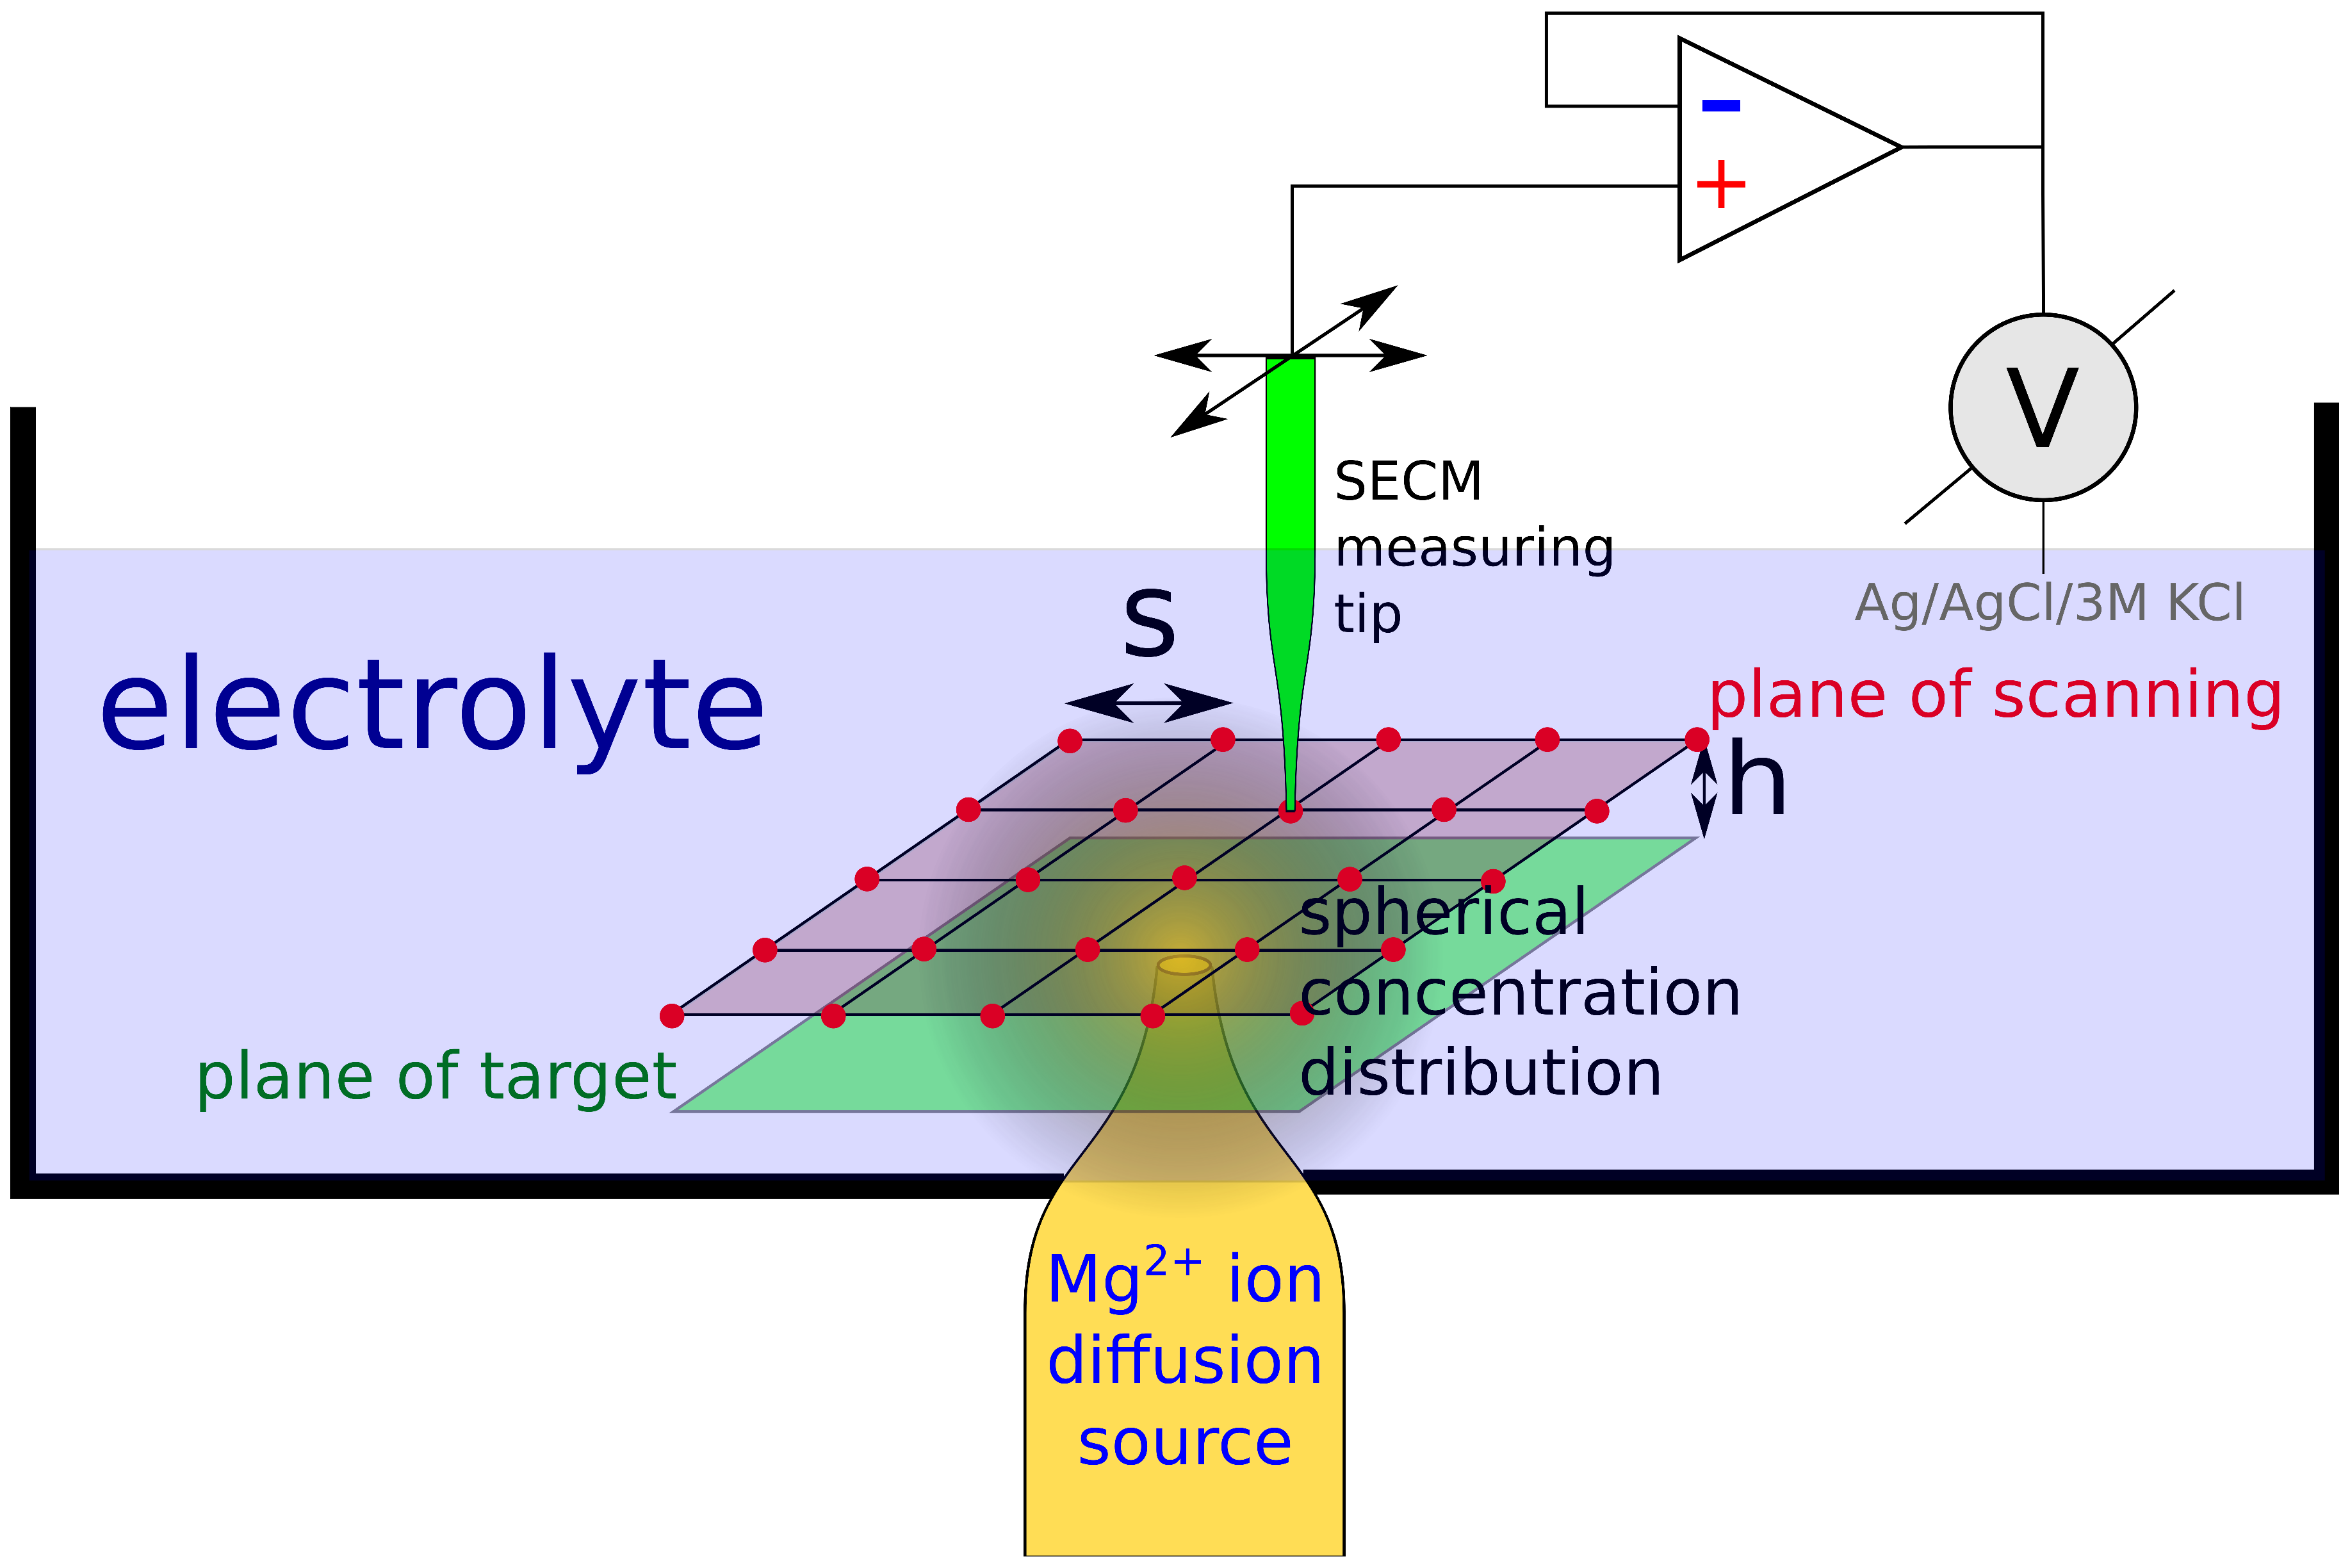
\includegraphics[width=0.8\textwidth]{img/setup.eps}\vspace{5mm}

\begin{flushleft}
\hspace{1.5cm} B
\end{flushleft}

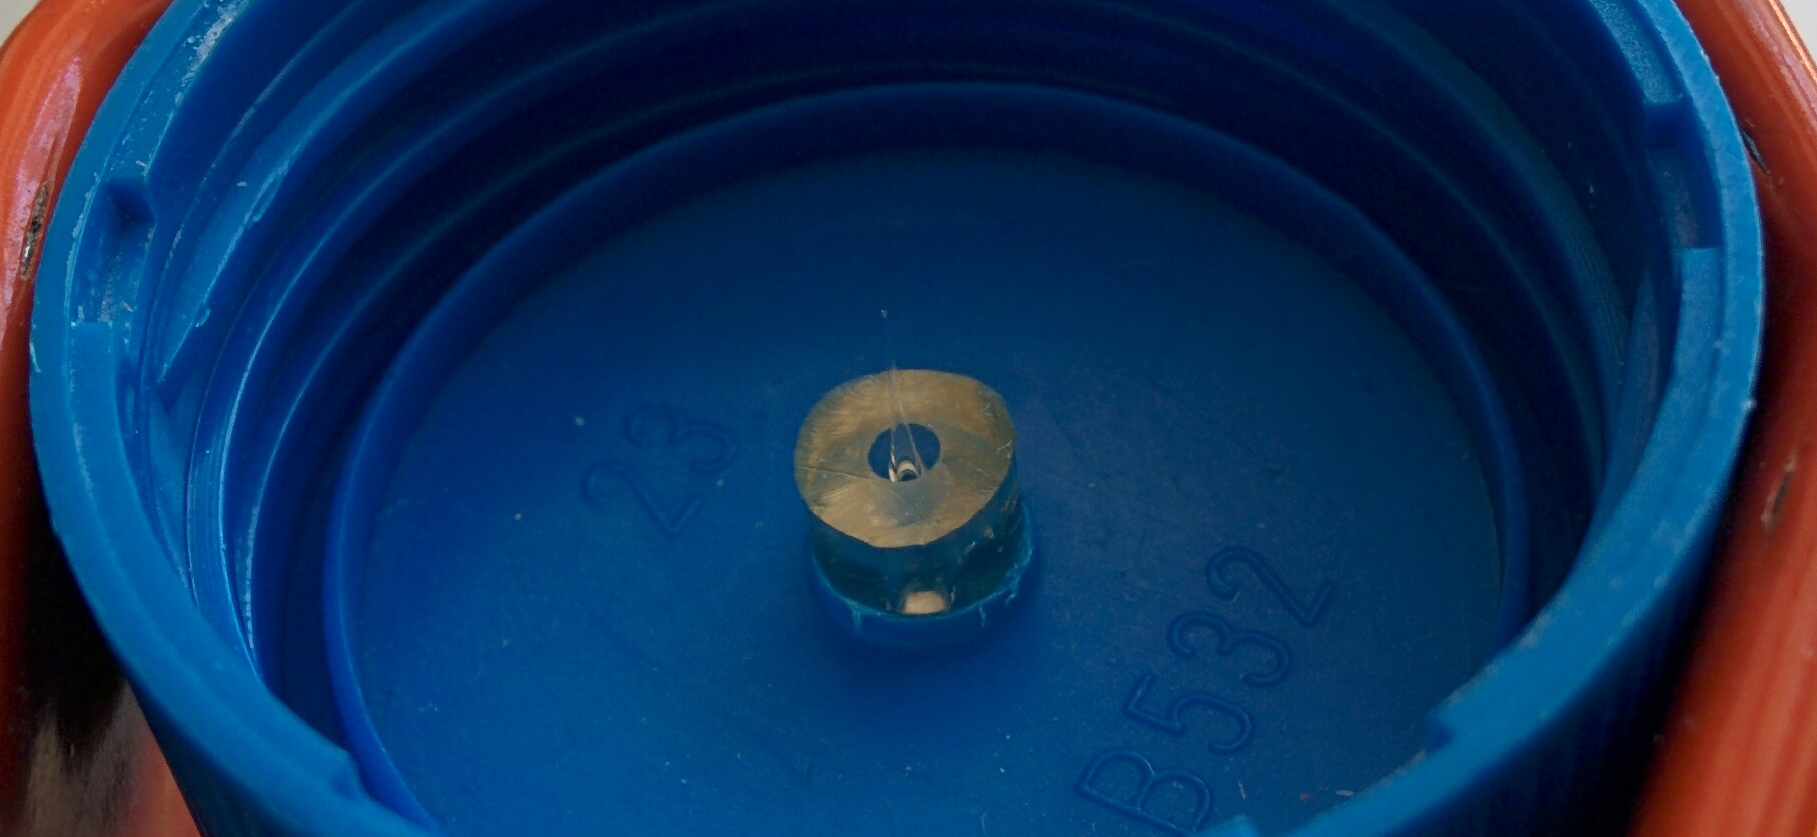
\includegraphics[width=0.7\textwidth]{img/pipette_source.jpg}
\caption[Sketch and photo of the model system with the embedded glass pipette Mg$^{2+}$ or K$^+$ ion diffusion source, and the SECM scan setup.]{Sketch (A) and photo (B) of the model system with the embedded glass pipette Mg$^{2+}$ or K$^+$ ion diffusion source, and the SECM scan setup.
"$h$" is height of scan, the distance between the plane of the target (pipette orifice) and the SECM tip.
"$s$" is the step size, that is the distance between two neighbouring data aquisition points.
Red dots indicate the data aquisition points of the 2D raster scan pattern.
Not drawn to scale.}
\label{fig:setup}
\end{figure}

		\subsection{Moulded model targets}
The model targets described here are prepared by moulding the samples with Epofix resin.
The mould was prepared from cut-off portion of a Falcon-tube.
The samples were placed upside down into the empty mould, then the resin was poured in.
After curing, the front side -- which was facing downwards during the curing process -- was sanded off until the sample surfaces were exposed.
Then, the surface was polished with sandpapers with increasingly higher grit, from 600 to 4000.
Then polishing was continued with alumina slurry on wet polishing cloth.
Alumina particle size was 1 $\upmu$m, 0.3 $\upmu$m and 0.05 $\upmu$m.
Finally, the surface was cleaned and degreased with absolute ethanol.
Fig. \ref{fig:model} depicts a sketch of the model targets prepared with this method, and the SECM setup used with these targets.
While scanning, the front side of the mount faced upwards, and was surrounded laterally by a PVC plastic tubing, creating a small container holding about 5 mL of test electrolyte solution, and a Ag/AgCl/3M KCl reference electrode.
In this way, only the well-defined cross section of the samples were exposed to the electrolyte.


\begin{figure}
\centering

\begin{flushleft}
\hspace{1.5cm} A
\end{flushleft}

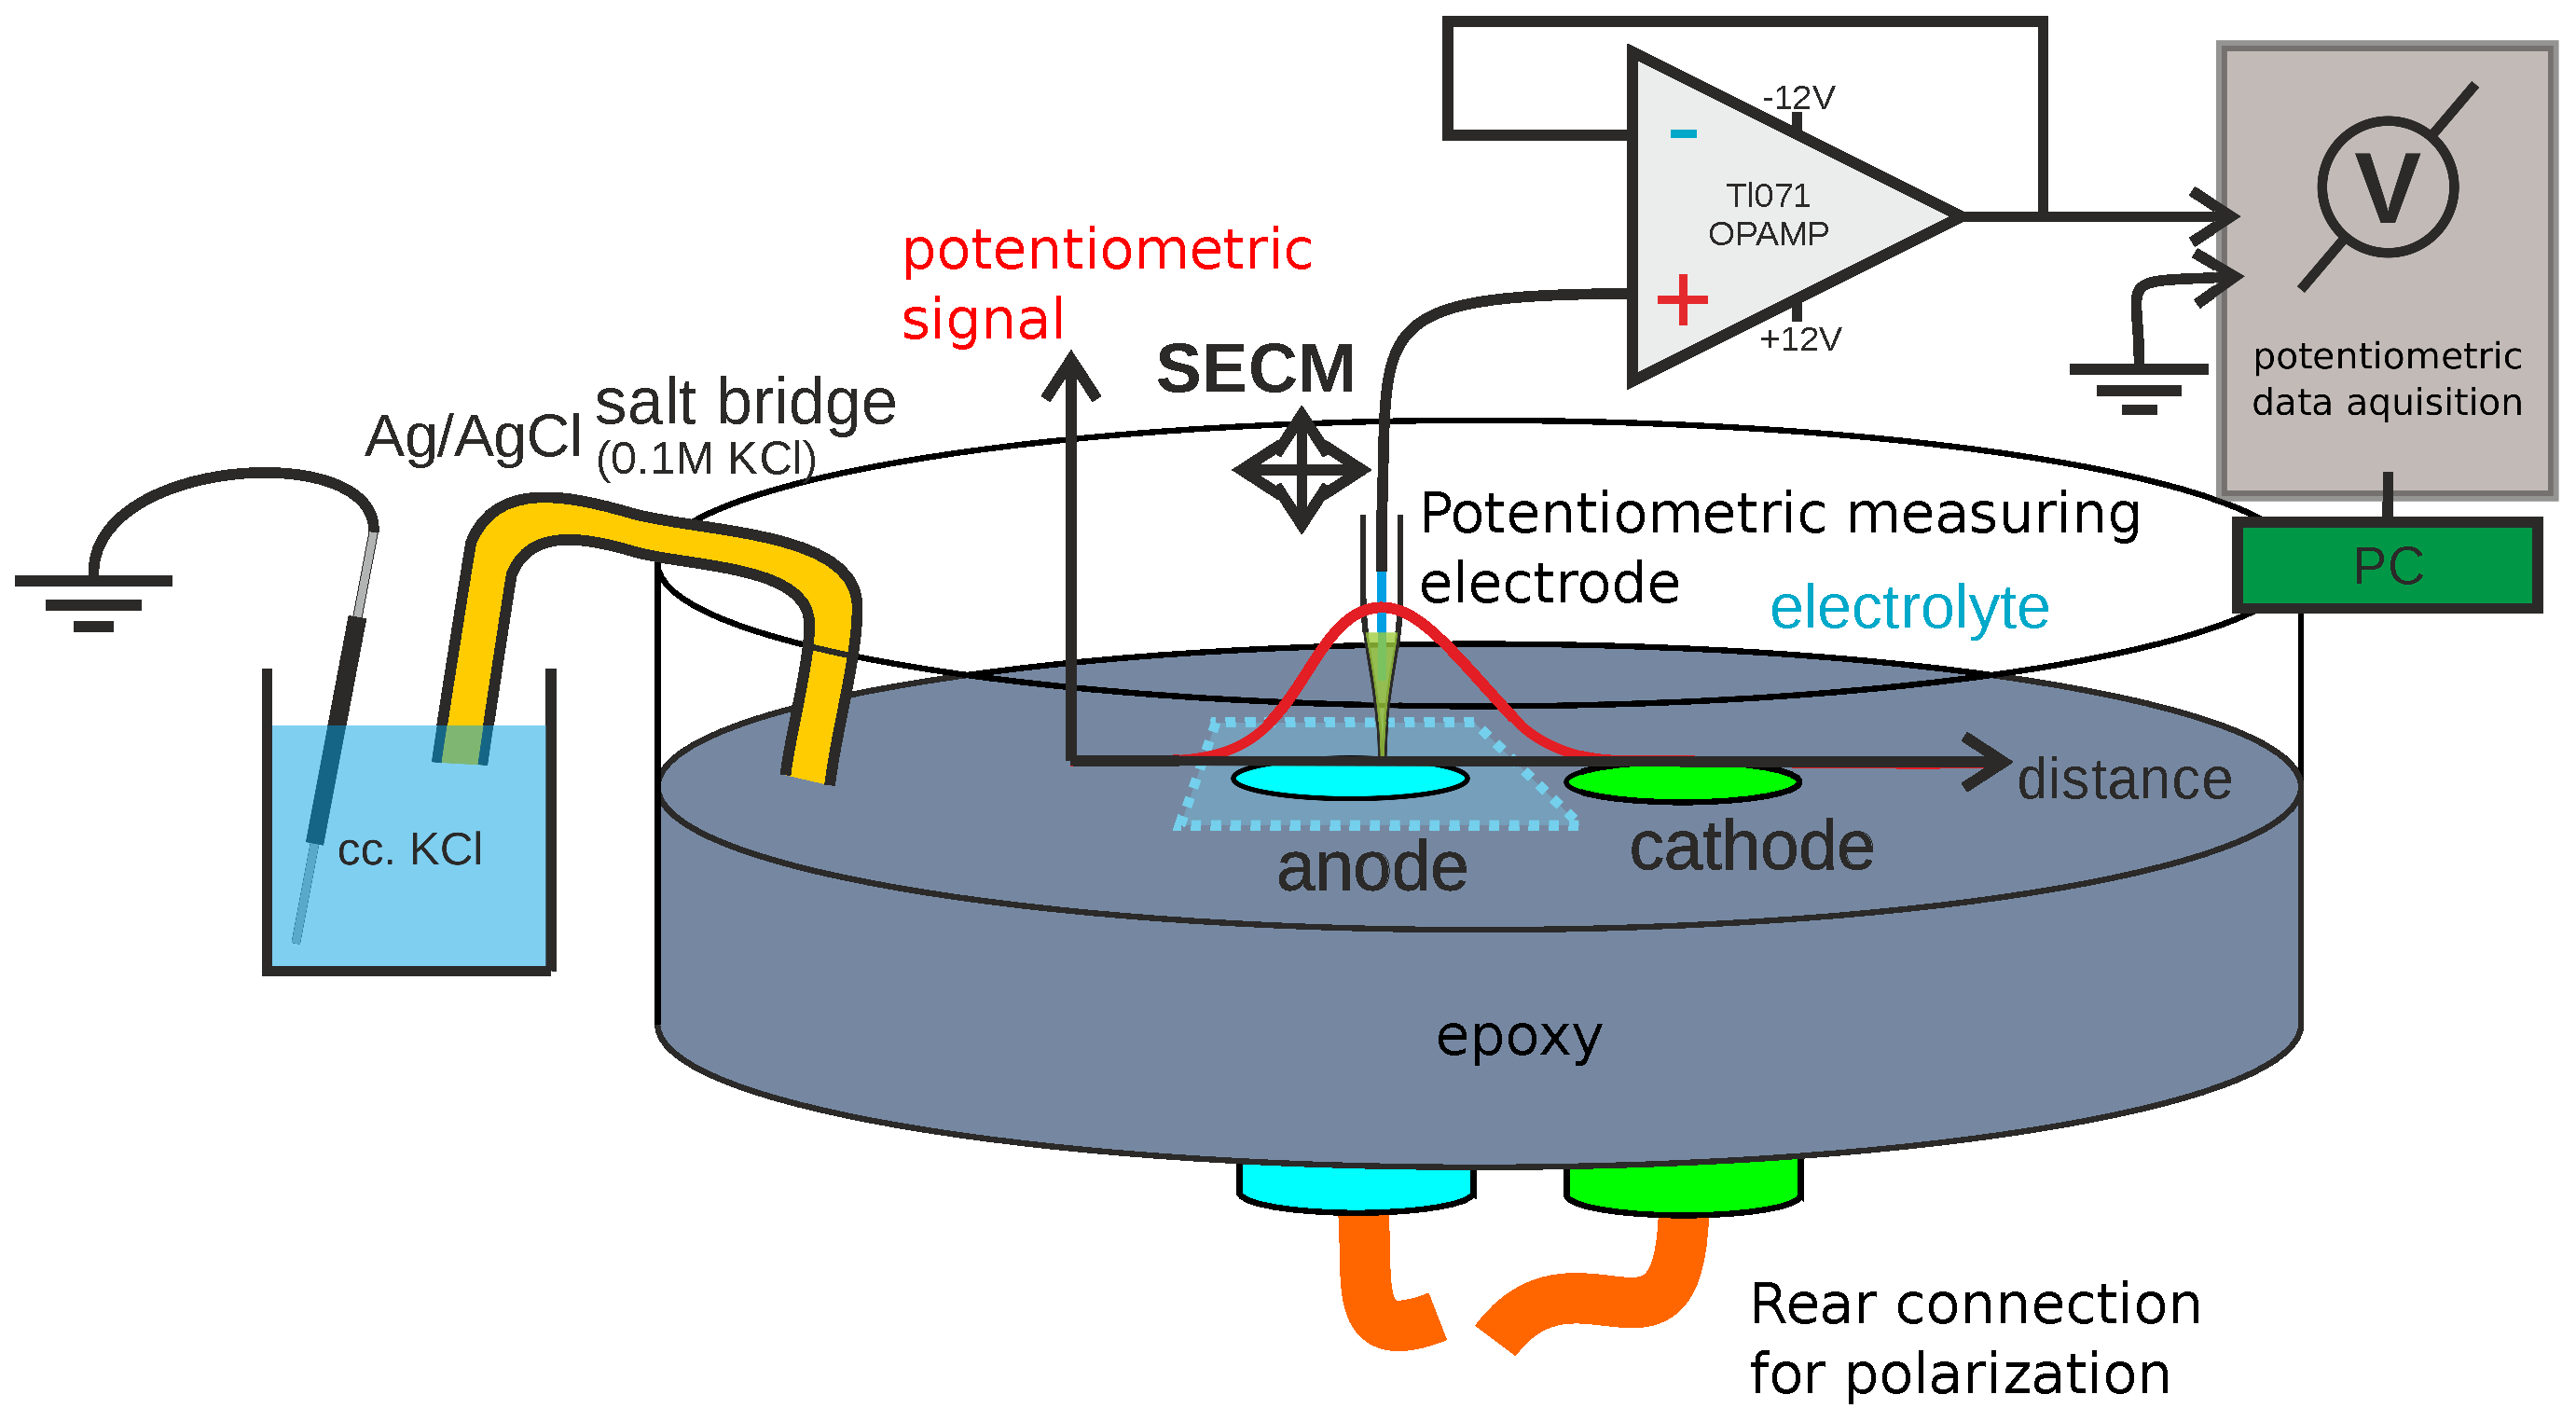
\includegraphics[width=0.8\textwidth]{img/model.eps}\vspace{5mm}

\begin{flushleft}
\hspace{1.5cm} B
\end{flushleft}

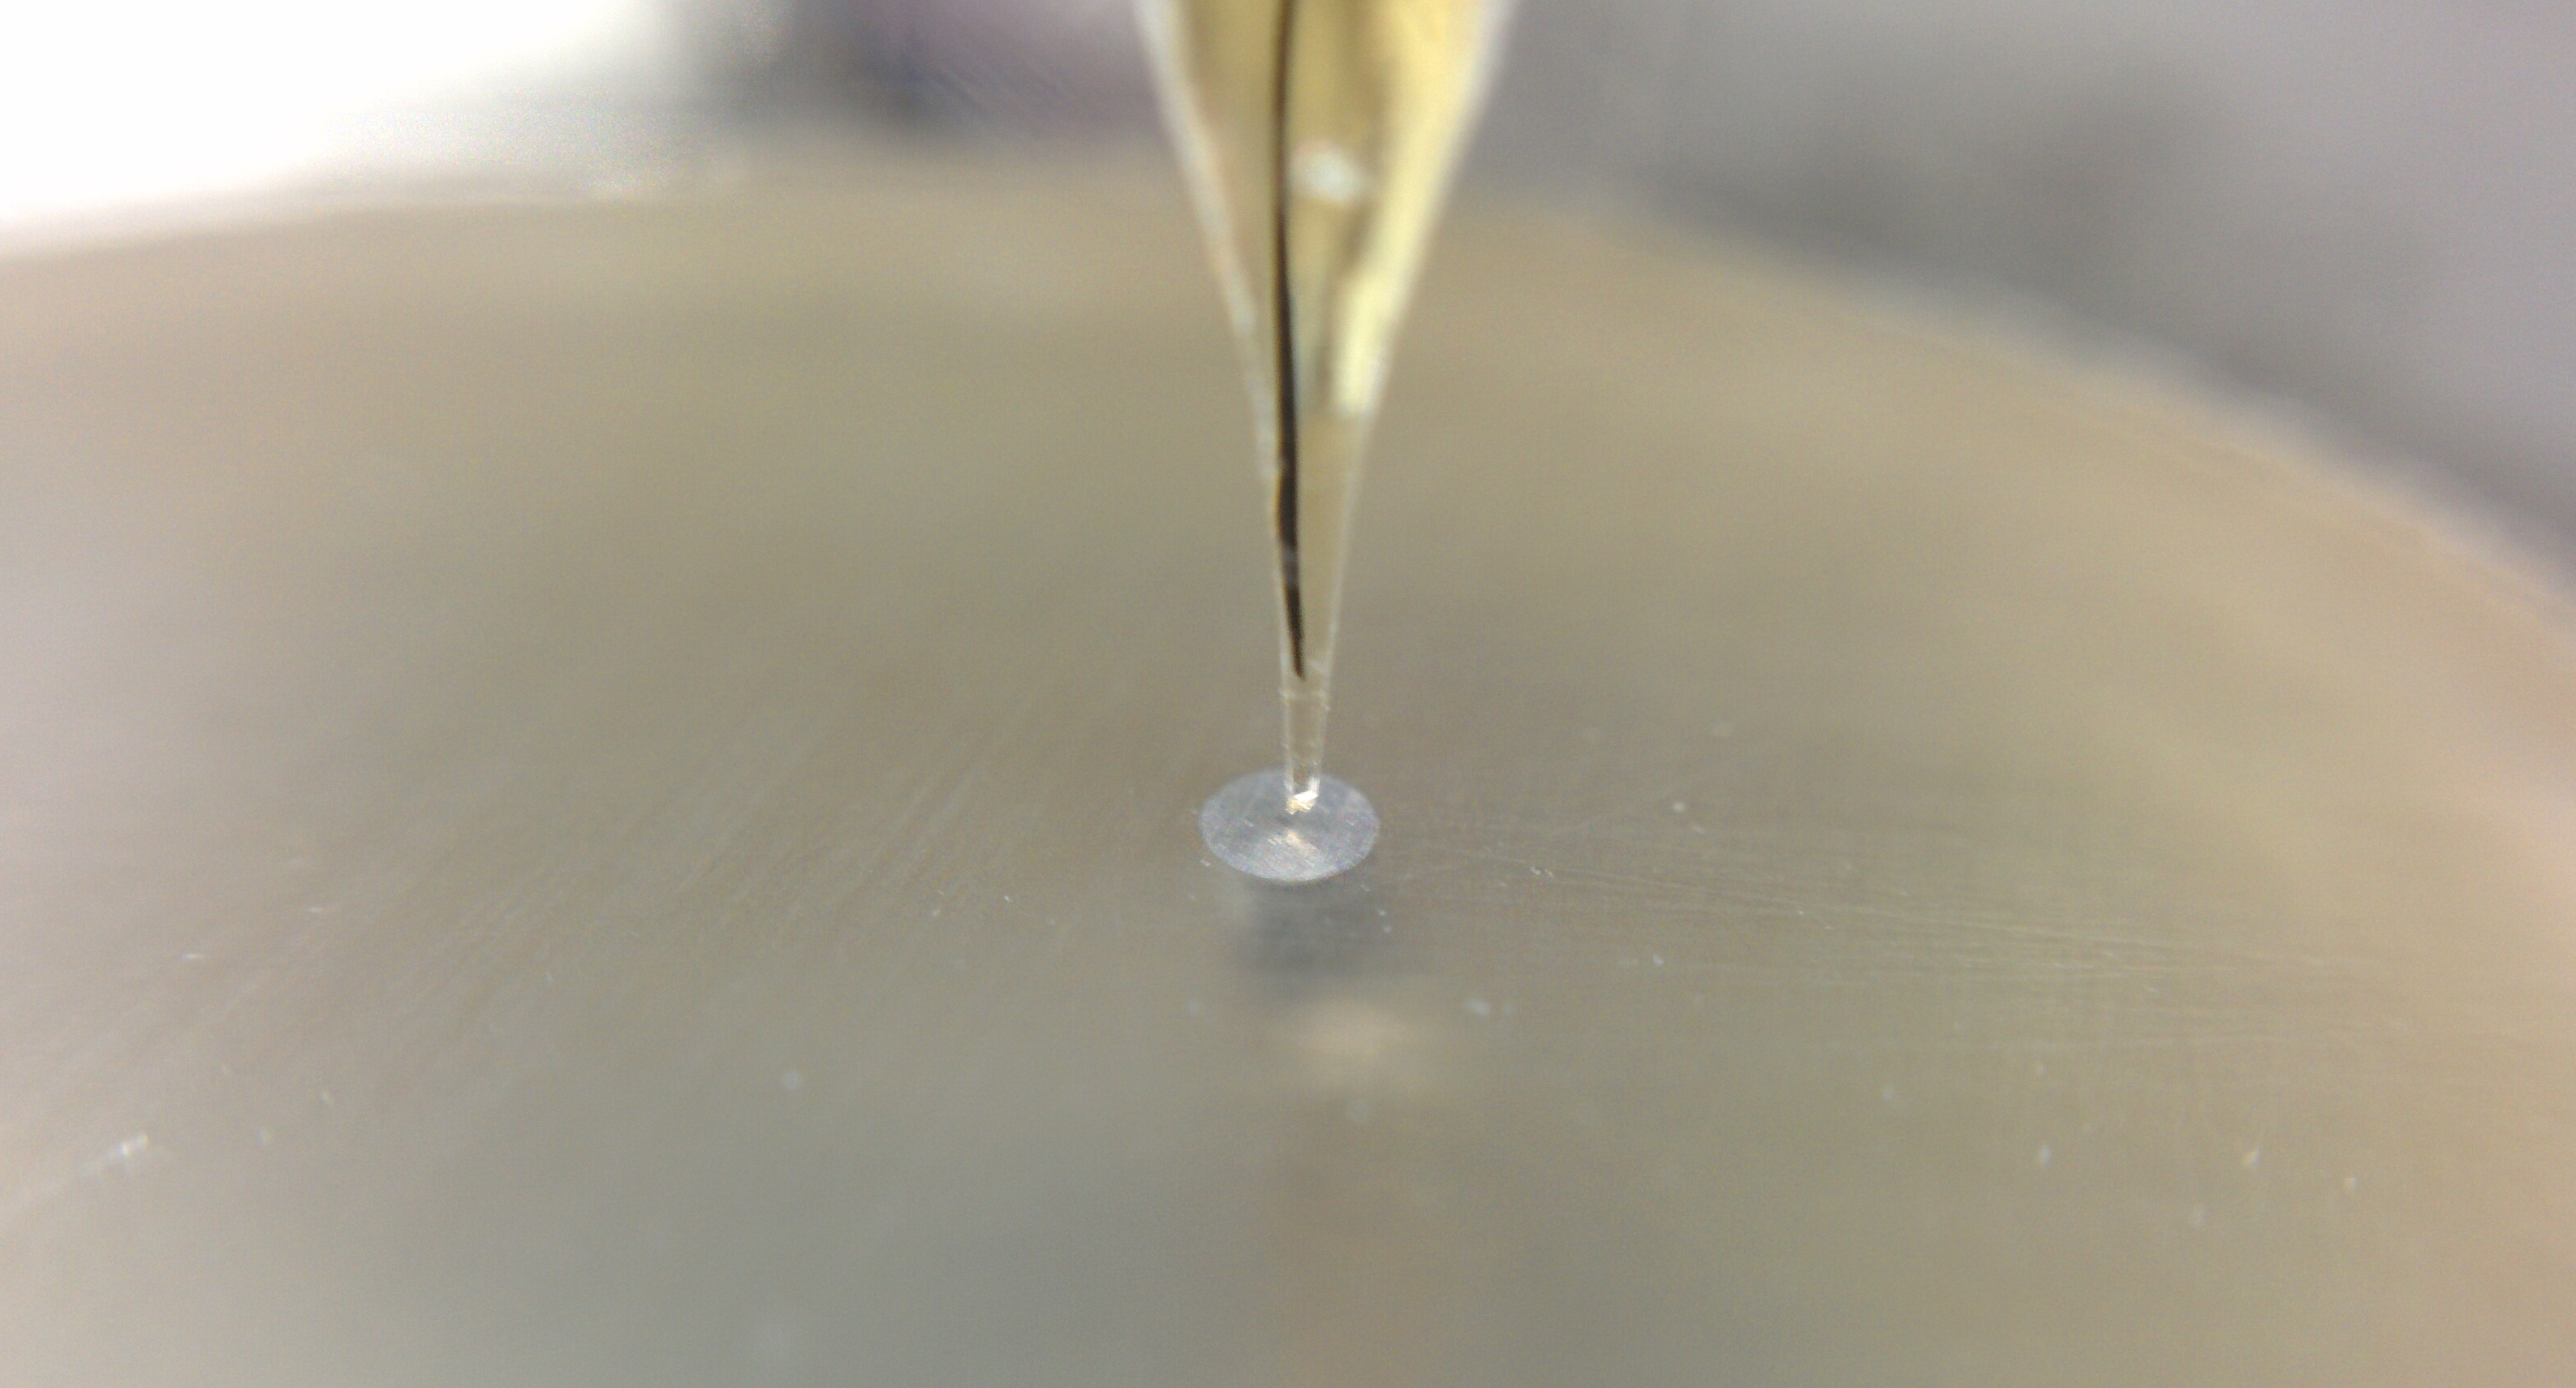
\includegraphics[width=0.6\textwidth]{img/model_photo.jpg}
\caption[Sketch of the moulded model targets and the SECM scan setup used for these targets.]{(A) Sketch of the moulded model targets and the SECM scan setup used for these targets. (B) Close-up photograph of the Mg$^{2+}$ ion selective microelectrode above the AZ63 sample.}
\label{fig:model}
\end{figure}

			\subsubsection{Iron -- magnesium galvanic couple}
A magnesium - iron galvanic couple was used as model corroding system.
An iron wire with a diameter of 760 $\upmu$m and a magnesium ribbon with a cross section of 200 $\upmu$m $\times$ 800 $\upmu$m were embedded in the Epofix resin disk.
Corrosive electrolyte was 1 mM NaCl.

			\subsubsection{Iron -- AZ63 galvanic couple}
Scans were also performed on an epoxy resin sleeve holding 760 $\upmu$m diameter wires of pure iron and AZ63 magnesium alloy, manufactured from a boyler sacrificial anode with a high-precision lathe.
The composition of the alloy was determined (in wt.\%) by colleagues from the \emph{University of La Laguna, Spain}, by emission spectrometry (ICP-OES): Al 5.74, Zn 2.88, Cu < 0.005, Fe < 0.005, Ni < 0.005, Si < 0.005, Mg balance \cite{souto2013spatially}.
Tests were conducted in 1 mM NaCl solution, naturally aerated, and at ambient temperature.

\begin{figure}
\centering
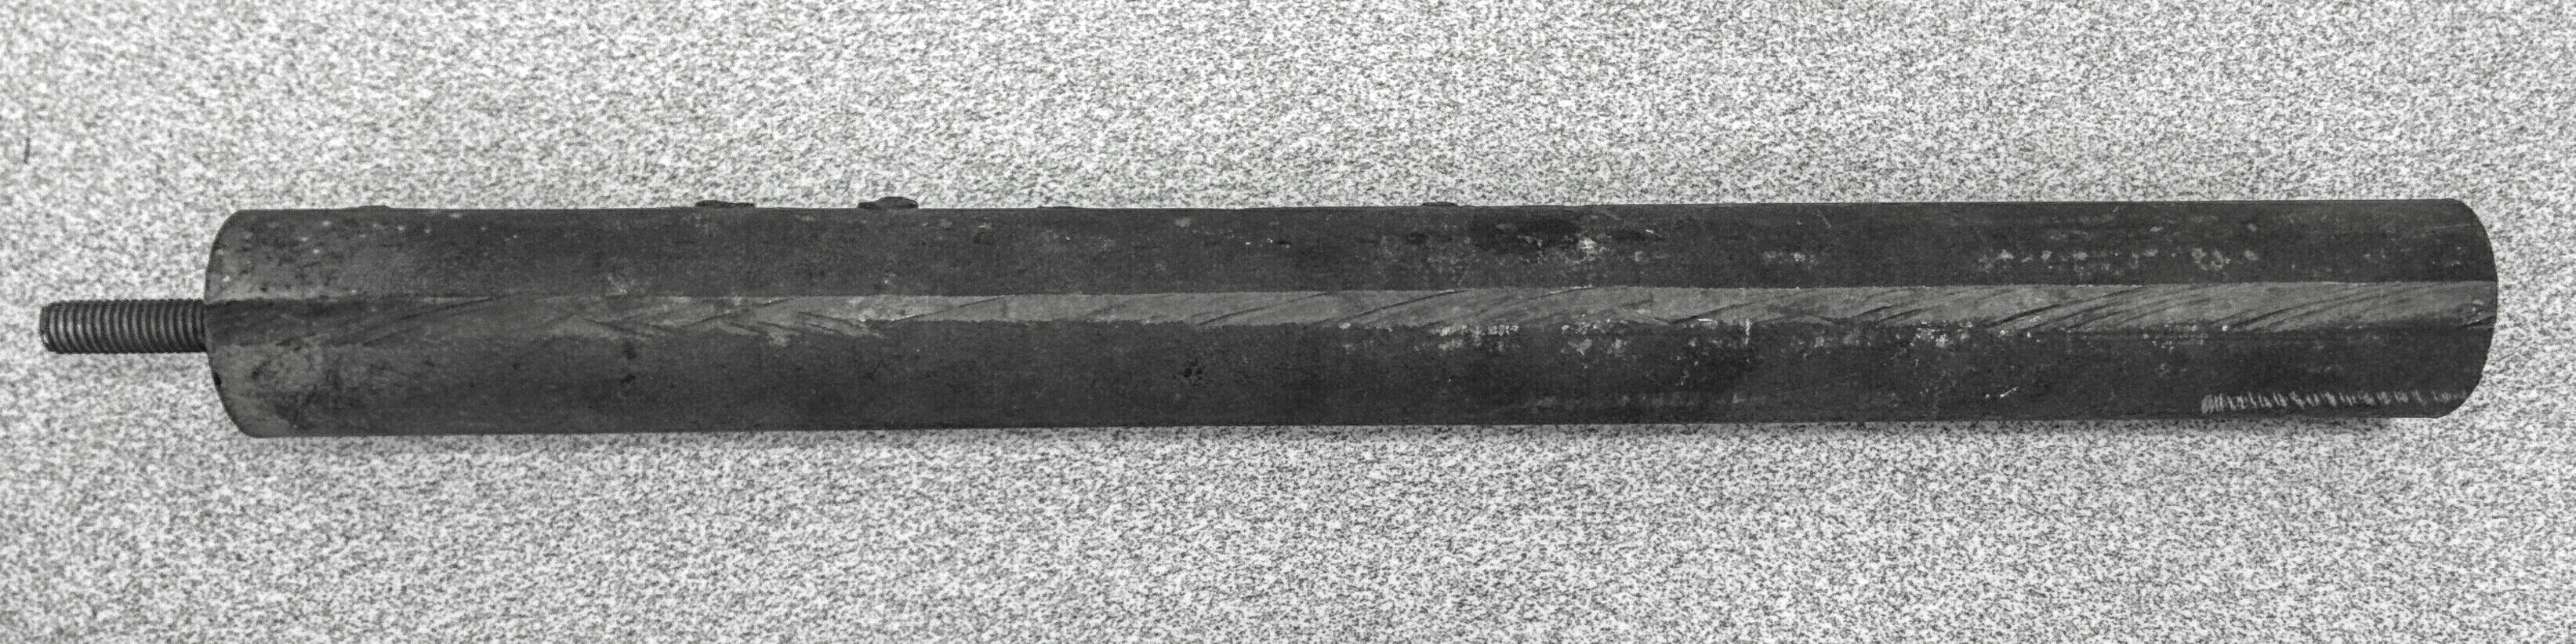
\includegraphics[width=0.7\textwidth]{img/az63.jpg}
\caption{The water heater sacrificial anode made of the AZ63 magnesium-aluminium-zinc alloy.
The sample was prepared from such an anode by a precision lathe.}
\label{fig:az63}
\end{figure}
			
			\subsubsection{Carbon steel}
The embedded sample in this case was a carbon steel (A $\approx$ 0.2 cm$^2$) JIS G3131 SPHC specimen with the composition, C: 0.04\%, Mn: 0.15\%, P: 0.026\%, S: 0.005\%, and Si: 0.02\% \cite{el2016secm}.

			\subsubsection{Graphite model target}
To demonstrate and compare the new scanning algorithms, images of pH-de\-pen\-dent potential profiles were recorded $h$ = 100 $\upmu$m above a graphite disc electrode, set to 2 V versus another, identical graphite electrode.
$d$ = 350 $\upmu$m mechanical pencil leads (Rotring, Hamburg, Germany) were used as graphite electrodes.
They were both embedded in the epoxy resin sleeve.
At this potential difference, pH of the electrolyte will decrease at the anode, and increase at the cathode, as a consequence of water electrolysis.
Electrolyte was unbuffered $10^{-3}$ M NaCl solution.
Potential image was recorded after 10 minutes of electrolysis.
During the imaging, the electrolysis cell was disconnected to avoid the electric field generated by the applied voltage affecting the image.
In this way a spherical concentration distribution is being generated above the target.

	\section{SECM routines}
		\subsection{For the comparison of solid and liquid contact microelectrodes}
2D scans were performed 100 $\upmu$m above the micropipette and the magnesium ribbon target.
Scanrate was 12.5 $\upmu$m/s in both cases.
Step size in $X$ and $Y$ direction was 25 and 50 $\upmu$m.
Scanned area was 1000 $\upmu$m $\times$ 1500 $\upmu$m ($X\times Y$).
Scanning probes were liquid and solid contact Mg$^{2+}$ ion-selective micropipettes.
A Sensolytics SECM system was used, potential was recorded with an Autolab Electrochemical workstation.
The TL082 voltage based follower was insterted between the measuring microelectrode and the Autolab.
Reference electrode was an Ag/AgCl/3 M KCl electrode.
		\subsection{Optimization of scanning patterns and algorithms}
			\subsubsection{Cartesian coordinate-system based patterns and algorithms}
The three conventional scanning algorithms are the meander, the comb, and the fast comb.
In meander, the probe travels through all of the raster coordinates without repetition and wasted movement, by alternating the $X$ scan direction from line to line, resulting in a characteristic ,,meander'' pattern.
In the comb pattern, the probe sweeps through each scan line twice, back and forth, then the two scans are averaged.
The fast comb algorithm scans only in one direction, and before advancing in the $Y$ direction, the probe travels back to the beginning of the scan line without measuring or stopping at all.


\begin{figure}
\centering
\begin{tikzpicture}
\begin{axis}    [unit vector ratio*=1 1 1,
                xmin=-1100,
                xmax=1100,
                ymin=-1100,
                ymax=1100,
                width=8cm,
                %height=9cm,
                xlabel={x, $\upmu$m},
                ylabel={y, $\upmu$m},
                clip marker paths=true,
		/pgf/number format/.cd, use comma, 1000 sep={}]
\addplot [color=red, mark=*, mark size=1] table {data/scanning_patterns/meander_pattern.txt};
\filldraw[fill=blue, draw=blue] (axis cs:-1000,-1000) circle (4);
\filldraw[fill=green, draw=green] (axis cs:1000,1000) circle (4);
\filldraw[fill=white, draw=white] (axis cs:-900,900) circle (5);
\node[anchor=center] at (axis cs:-900,900) {A};
\end{axis}
\end{tikzpicture}
\hfill
\begin{tikzpicture}
\begin{axis}    [unit vector ratio*=1 1 1,
                xmin=-1100,
                xmax=1100,
                ymin=-1100,
                ymax=1100,
                width=8cm,
                %height=9cm,
                xlabel={x, $\upmu$m},
                ylabel={y, $\upmu$m},
                clip marker paths=true,
		/pgf/number format/.cd, use comma, 1000 sep={}]
\addplot [color=red, mark=*, mark size=1] table {data/scanning_patterns/fastcomb_pattern.txt};
\filldraw[fill=blue, draw=blue] (axis cs:-1000,-1000) circle (4);
\filldraw[fill=green, draw=green] (axis cs:1000,1000) circle (4);
\filldraw[fill=white, draw=white] (axis cs:-900,900) circle (5);
\node[anchor=center] at (axis cs:-900,900) {B};
\end{axis}
\end{tikzpicture}

\begin{tikzpicture}
\begin{axis}    [unit vector ratio*=1 1 1,
                xmin=-1100,
                xmax=1100,
                ymin=-1100,
                ymax=1100,
                width=8cm,
                %height=9cm,
                xlabel={x, $\upmu$m},
                ylabel={y, $\upmu$m},
                clip marker paths=true,
		/pgf/number format/.cd, use comma, 1000 sep={}]
\addplot [color=red, mark=*, mark size=1] table {data/scanning_patterns/comb_pattern.txt};
\filldraw[fill=blue, draw=blue] (axis cs:-1000,-1000) circle (4);
\filldraw[fill=green, draw=green] (axis cs:-1000,1000) circle (4);
\filldraw[fill=white, draw=white] (axis cs:-900,900) circle (5);
\node[anchor=center] at (axis cs:-900,900) {C};
\end{axis}
\end{tikzpicture}
\hfill
\begin{tikzpicture}
\begin{axis}    [unit vector ratio*=1 1 1,
                xmin=-1100,
                xmax=1100,
                ymin=-1100,
                ymax=1100,
                width=8cm,
                %height=9cm,
                xlabel={x, $\upmu$m},
                ylabel={y, $\upmu$m},
                clip marker paths=true,
		/pgf/number format/.cd, use comma, 1000 sep={}]
\addplot [color=red, mark=*, mark size=1] table {data/scanning_patterns/web_pattern.txt};
\filldraw[fill=blue, draw=blue] (axis cs:0,0) circle (4);
\filldraw[fill=green, draw=green] (axis cs:809,-588) circle (4);
\filldraw[fill=white, draw=white] (axis cs:-900,900) circle (5);
\node[anchor=center] at (axis cs:-900,900) {D};
\end{axis}
\end{tikzpicture}

\begin{tikzpicture}
\begin{axis}    [unit vector ratio*=1 1 1,
                xmin=-1100,
                xmax=1100,
                ymin=-1100,
                ymax=1100,
                width=8cm,
                %height=9cm,
                xlabel={x, $\upmu$m},
                ylabel={y, $\upmu$m},
                clip marker paths=true,
		/pgf/number format/.cd, use comma, 1000 sep={}]
\addplot [color=red, mark=*, mark size=1] table {data/scanning_patterns/arc_pattern.txt};
\filldraw[fill=blue, draw=blue] (axis cs:0,0) circle (4);
\filldraw[fill=green, draw=green] (axis cs:995,-101) circle (4);
\filldraw[fill=white, draw=white] (axis cs:-900,900) circle (5);
\node[anchor=center] at (axis cs:-900,900) {E};
\end{axis}
\end{tikzpicture}

\caption[Scanning algorithms.]{The conventional (A) meander, (B) fast comb and (C) comb, and the new, proposed (D) web, and (E) arc SECM scanning patterns for circularly symmetric targets. Red dots indicate sampling points, red line shows the probe path.
Blue and green dots indicate starting and finishing positions, respectively.}
\label{fig:patterns}
\end{figure}

In the meander, fast-comb, and comb algorithms, total scanned area was $2000~\upmu$m $\times$ $2000~\upmu$m, resolution was 100 $\upmu$m $\times$ 100 $\upmu$m, and consequently 21 $\times$ 21 = 441 raster points altogether. 
 
Both in the experimental and simulated SECM scans, for each point, 1 second was split between probe movement, resting period, and signal sampling.
One measurement was performed at every point after the resting period, before positioning the probe to the next point.
Probe movement speed was 312.5 $\upmu$m/s.
The starting position was $x = -1000~\upmu$m, $y = -1000~\upmu$m.

			\subsubsection{Circular, polar-coordinate system based patterns and algorithms}
The two new scanning patterns proposed in this thesis are called the ,,web'' and the ,,arc'' patterns.
In the web pattern, sampling points are located on concentric circles with regularly increasing radius.
On each circle, there are equal number of points.
The first point in each circle has the angular coordinate of 0$^{o}$, which increases at regular intervals with the rest of the points.
Using this pattern, resolution decreases as radius increases.
The arc pattern is very similar, except that the points on the circles are separated by equally long arcs, so that with increasing radius, the number of points increases, and resolution is maintained.
The scanning patterns can be seen in Figure \ref{fig:patterns}.

In the web algorithm, the radius of the scanned area was $r$ = 1000 $\upmu$m, with $\Delta r$ = 100 $\upmu$m, and $\Delta \alpha$ = 2$\pi$/10 radians, resulting in 10 points on each circle, and a total of 110 points.
In the arc pattern $r$ and $\Delta r$ was the same as in the web pattern, arc distance between adjacent points along the circles was 100 $\upmu$m, with a total of 341 points.

Starting position was $x$ = 0 $\upmu$m, $y$ = 0 $\upmu$m relative to the target center for both algorithms.

The images obtained with the two polar coordinate-based algorithms were interpolated to the grid points of the 2D raster used by the other algorithms to allow similar visualization.

	\subsection{SECM routines for the deconvolution study}
		\subsubsection{Linescans}

To examine the effect of equilibration interval length on the image distortion, and for easy comparison of raw and deconvoluted data, line scans were recorded with three different time intervals allocated for each data aquisition point: 0.5 s, 2$~$s, and 5$~$s.
Probe movement speed was 1000 $\upmu$m/s, and therefore probe movement interval was 0.1 s, resulting in equilibration interval lengths ($t_e$) of 0.4 s, 1.9 s, and 4.9 s, respectively.
Step size was 100$~\upmu$m, scan distance was 2000 $\upmu$m with the source center in the middle.
8 consecutive line scans (4 forward and 4 reverse scans) were performed in each case to confirm repeatability.

		\subsubsection{2D scans}
To confirm the effect of deconvolution on 2D image quality, 2D raster scans were performed with four different equilibration interval lengths (4.9 s, 1.9 s, 0.9 s, 0.4 s), and two different scanning algorithms; the meander and the fast comb.
In meander, the probe travels through all of the raster coordinates without repetition and wasted movement, by alternating the X scan direction from line to line, resulting in a characteristic ,,meander'' pattern.
The fast comb algorithm scans only in one direction, and before advancing in the Y direction, the probe travels back to the beginning of the scan line without measuring or stopping at all (paper \textbf{IV}).

Starting position was $X = -1000$ $\upmu$m, $Y = -1000$ $\upmu$m.
Both algorithms used horizontal scanning.
Initial scan direction for the meander algorithm, and scan direction for the fast comb algorithm was left to right.
Step size was 100 $\upmu$m, scanned area was 2000 $\upmu$m $\times$ 2000 $\upmu$m, resulting in overall scanning times of 2205 s, 882 s, 441 s, and 220.5 s.

In the experiments with the micropipette sources, the $X = 0$ $\upmu$m, $Y = 0$ $\upmu$m reference position was established by positioning the measuring tip 100 $\upmu$m above the orifice center of the diffusion source, with the aid of a camera.
Then, the tip was positioned at the starting coordinates, and the electrolyte was introduced to the cell.
10 minutes later, the scan was started. 

		\subsection{Backlash compensation}
To rule out additional distortion caused by the SECM apparatus, backlash of the linear stages was measured and found to be below 1 $\upmu$m after software compensation.
To measure backlash, a microscope slide with a micrometer scale was fixed on the linear stage, then the stage was moved 1000 $\upmu$m to one direction, to make sure the momentary backlash in that direction is zero.
After taking a photo, the stage was moved 100 $\upmu$m to the same direction, and another photo was taken.
Then, the stage was moved 100 $\upmu$m to the opposite direction, and a photo was taken again.
The difference between the first and last photo is the backlash of the particular stage.
Fig. \ref{fig:backlash} shows the photos for each stage of the home-made SECM.

\begin{figure}
\centering
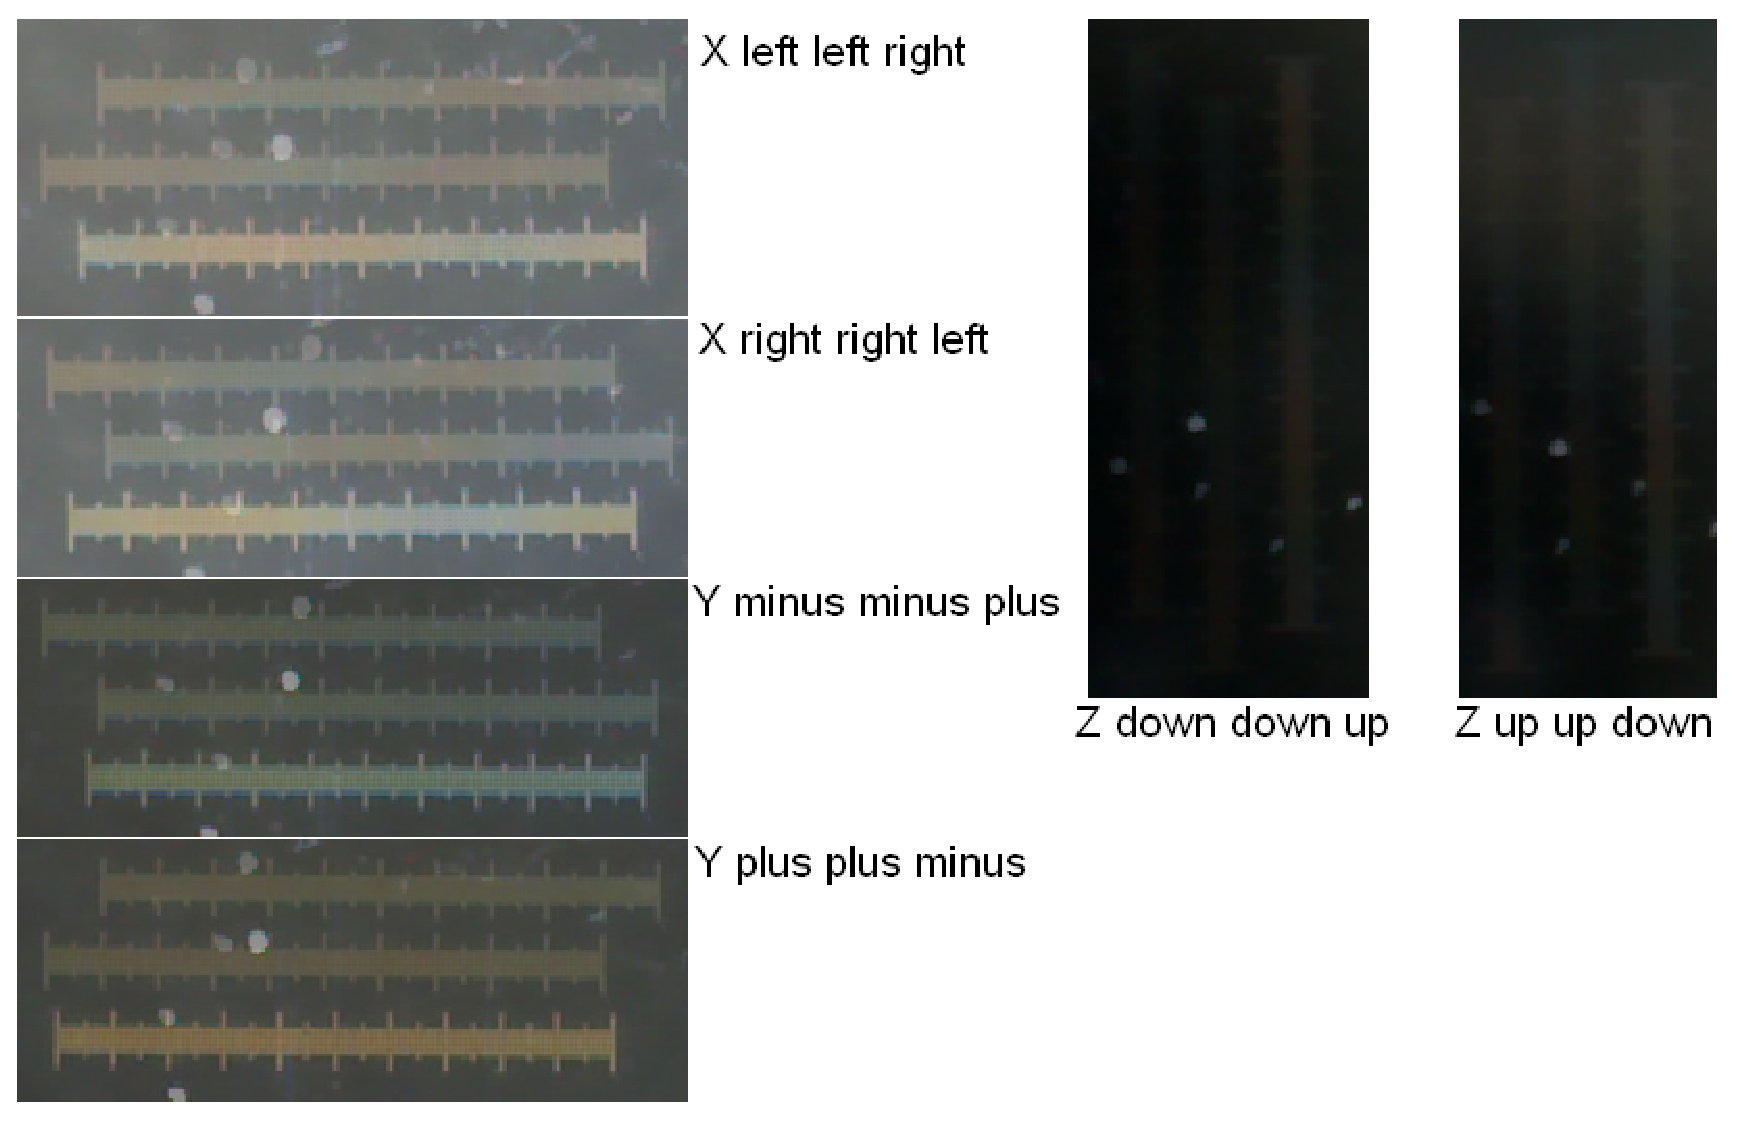
\includegraphics[width=0.8\textwidth]{img/backlash.eps}
\caption[Microphotos for the backlash compensation measurements for the home-made SECM.]{Microphotos for the backlash compensation measurements for the home-made SECM.
The photos show a microscope slide with a micrometer scale fixed on the microelectrode holder.
Labels ("left", "right") indicate the direction of the slide unit movement prior to taking the microphoto.
First, the slide unit was moved 1000 $\upmu$m, the a photo was taken.
Then, it was moved 100 $\upmu$m in the same direction, and another photo was taken.
Finally, it was moved in the opposite direction 100 $\upmu$m, and a photo was taken.
The difference between the second and the third photo is the backlash, which was compensated through the control software.}
\label{fig:backlash}
\end{figure}

	\section{Deconvolution of potentiometric SECM images}
The potentiometric signal-time response function to change in analyte activity can be characterized with the time constant.
It is the time required for the cell potential difference to change from its initial value by the fraction $1-e^{-1} = 0.63$ of the final value \cite{mcnaught1997compendium}.
The cell can be modeled as a simple $RC$ low-pass filter arranged serially between the signal input and the output \cite{halliwell1987using}.
In this case, time constant is $\tau$ = $RC$, where $R$ is the resistance of the cell with the largest contribution from the measuring electrode, and $C$ is the capacitance of the cell with the largest contribution from the input amplifier and the cable between the amplifier and the electrodes.

Eq. \ref{eq:rc} describes the transient cell response when the measuring electrode is brought to contact with a solution of different analyte activity.

\begin{equation}
\label{eq:rc}
        E_{cell}(t) = E_{cell}(\infty) + [E_{cell}(0) - E_{cell}(\infty)]e^{-t/RC}
\end{equation}
where $E_{cell}(t)$ is the cell potential difference at time $t$, $E_{cell}(\infty)$ is the equilibrium cell potential difference, $E_{cell}(0)$ is the cell potential difference prior to the change. From this, $E_{cell}(\infty)$ can be expressed as:

\begin{equation}
\label{eq:rc2}
        E_{cell}(\infty)
        =
        \frac
                {E_{cell}(t) - E_{cell}(0)e^{-t/RC}}
                {1 - e^{-t/RC}}
\end{equation}

This can be used as a deconvolution function for potentiometric SECM images, substituting the time that elapses between two consecutive measurements in the SECM scan for $t$ to calculate each equilibrium $E_{cell}(\infty)$ from the respective observed $E_{cell}(t)$ potential difference values.

When the tip advances from the $i$th data acquisition point to the $(i+1)$th, cell potential difference changes from the initial $E_{cell}(t, i)$ to $E_{cell}(t, i+1)$.
Therefore, for every point, $E_{cell}(0, i)$ will be equal to $E_{cell}(t, i-1)$.
To deconvolute the raw image, the following calculation kernel was cycled through the data matrix points in the same order as they were recorded in the scan:


\begin{equation}
\label{eq:rc3}
        E_{cell}(\infty, i)
        =
        \frac
                {E_{cell}(t, i) - E_{cell}(t, i-1)e^{-t/RC}}
                {1 - e^{-t/RC}}
\end{equation}

$RC$ time constant in Eq. \ref{eq:rc2} was substituted with the value calculated from $R\times C$, obtained in the measurements described in the previous subsection.
A FORTRAN program was written to perform the deconvolution:

\begin{lstlisting}
program deconvolution
implicit none
integer :: i, j, stat
real rc, e0, conv
real t
rc=0.85
open(1,file='data.txt')
open(2,file='data_deconvoluted.txt')
read(1, *) i, j, e0
do
   read(1, *, iostat=stat) i, j, conv
   if (stat /= 0) exit
   write(2, *) i, j, ((conv - e0*rc)/(1-rc))
   e0=conv
end do
close(1)
close(2)
end program deconvolution
\end{lstlisting}

	
	\section{Simulation of the SECM measurements}
		\subsection{3D numerical simulation of diffusion from a disk source}
For the diffusion simulation, the \emph{,,point''} variant of the finite difference method was used as described in \cite{britzdigital}.
In potentiometric SECM, the tip is a passive probe, it does not generate or collect, therefore it does not alter the concentration profile of the species generated at the substrate.
The model target can be implemented in simulation by a disk surface with a constant flux of the generated species, H$_3$O$^{+}$.
Since the probe is passive, the concentration profile is only affected by the magnitude of the flux, and the diffusion coefficient of the species.
The time dependent diffusion problem is described by Fick's Second Law of Diffusion:

\begin{equation}
\label{eq:fick2}
        \frac
                {\partial c}
                {\partial t}
                =
                D
                \nabla^2c
\end{equation}
where $c$ is the concentration, $t$ is time, $D$ is the diffusion coefficient.
For three dimensions, Equation \ref{eq:fick2} can be expressed in discrete form for solving with the finite difference method as

\begin{equation}
\label{eq:3d}
	\begin{split}
	\frac   {c_{i,j,k}^{'} - c_{i,j,k}}{\delta t}
	=
	\frac {D} {h^2} (c_{i,j+1,k} + c_{i-1,j,k} + c_{i+1,j,k} + c_{i,j-1,k} + c_{i,j,k-1} + c_{i,j,k+1} - 6c_{i,j,k})
	\end{split}
\end{equation}
where $h$ is the distance between the adjacent points in space, $c_{i,j,k}$ is the concentration at the grid point with the coordinates of $i, j, k$, and $c_{i,j,k}^{'}$ is the same, but in the previous cycle, at the time instance $t-\delta t$.
This can be solved numerically for a given time instance by iterating Equation \ref{eq:3d} on every point of a 3D matrix, which represents the diffusion system.

The simulation model consisted of a cubic diffusion field with an edge length of 20 mm, and a resolution of 10 $\upmu$m on all three axes.
The top and side faces had Dirichlet boundary condition with $c$ = 0, representing the bulk solution.
The bottom face had a disc shaped source with a diameter of $d$ = 350 $\upmu$m, with Neumann boundary condition, to model the graphite anode, where H$_3$O$^{+}$ was being generated.
The rest of the bottom surface had Neumann boundary condition with a constant $j$ = 0 flux, modeling epoxy resin which embedded the graphite electrolysis electrode.
A FORTRAN program was written to calculate the potential profile for $t$ = 600 s.
A 2D section of the solved 3D diffusion matrix was taken at $h$ = 100 $\upmu$m, and it was normalized to $c_{max}$.
This was the input matrix for the SECM scanning simulation.

		\subsection{SECM scan simulation}
The SECM scan simulations were performed on a normalized 2D section of the solved 3D diffusion matrix.
The following calculation kernel was cycled through the data points using the same scanning algorithms as in the experimental SECM scans:

\begin{equation}
\label{eq:scan}
C_i = c_i + ( C_{i-1} - c_i ) \times T
\end{equation}
where $C_i$ and $c_i$ are the values of the $i$-th point in the output, and input matrices, respectively, $C_{i-1}$ is the value at the previous point, at $i-1$, and $T$ is a constant, equivalent of expression $e^{-t/RC}$ in Equation \ref{eq:rc}.
A value of 0.7 was set for $T$.
For $i$ = 1, $C_i$ was set to $c_i$, assuming the potentiometric cell was in equilibrium in the beginning of the scan simulation.

	\section{Scanning Electrochemical Microscope}
Throughout my work, I used three different SECM.
One was supplied by Sensolytics (Bochum, Germany).
The instrument was built around an Autolab (Metrohm, Herisau, Switzerland) electrochemical interface, controlled with a personal computer.
Amperometric, potentiostatic and potentiometric operations were available in this configuration.
A voltage follower based on a 10$^{12}\; \ohm$ input impedance operational amplifier (TL082, Texas Instruments) was introduced in the measuring circuit.
The cell voltages were measured with an electrometer and collected by the PC through the electrochemical interface.
The scanning system (Applicable Electronics Inc, New Haven, CT, USA) used a 3D micropositioner driven by precision stepping motors.
The distance between the scanning tip and the substrate was usually established by allowing the probe to gently touch the sample, and subsequently the probe was generally retracted to operation distance 100 $\upmu$m with the aid of the Z-positioning motor.
A video camera was used to further assist positioning of the tip close to the surface.
Raster scanning was employed to record the consecutive scan lines composing the XY grid.

The other two SECM were custom built at the University of Pécs.
While using these microscopes, potential was measured against an Ag/AgCl/3M KCl reference electrode with a high input impedance eDAQ pH/ISE isoPod USB (eDAQ Pty Ltd, Australia).

\begin{figure}
\centering
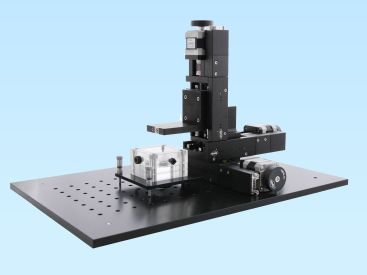
\includegraphics[width=0.3\textwidth]{img/sensolytics.jpg}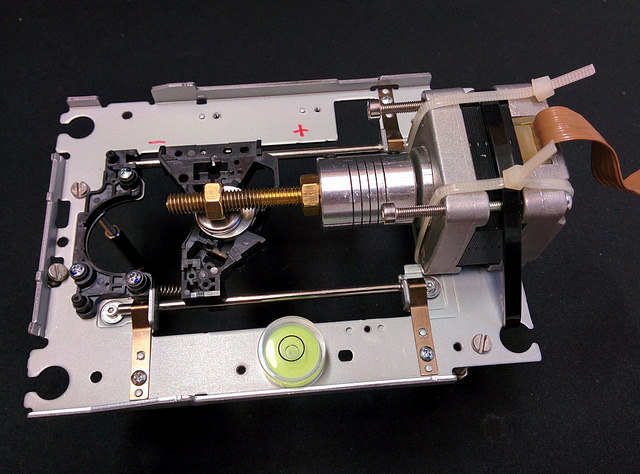
\includegraphics[width=0.3\textwidth]{img/diy_secm.jpg}

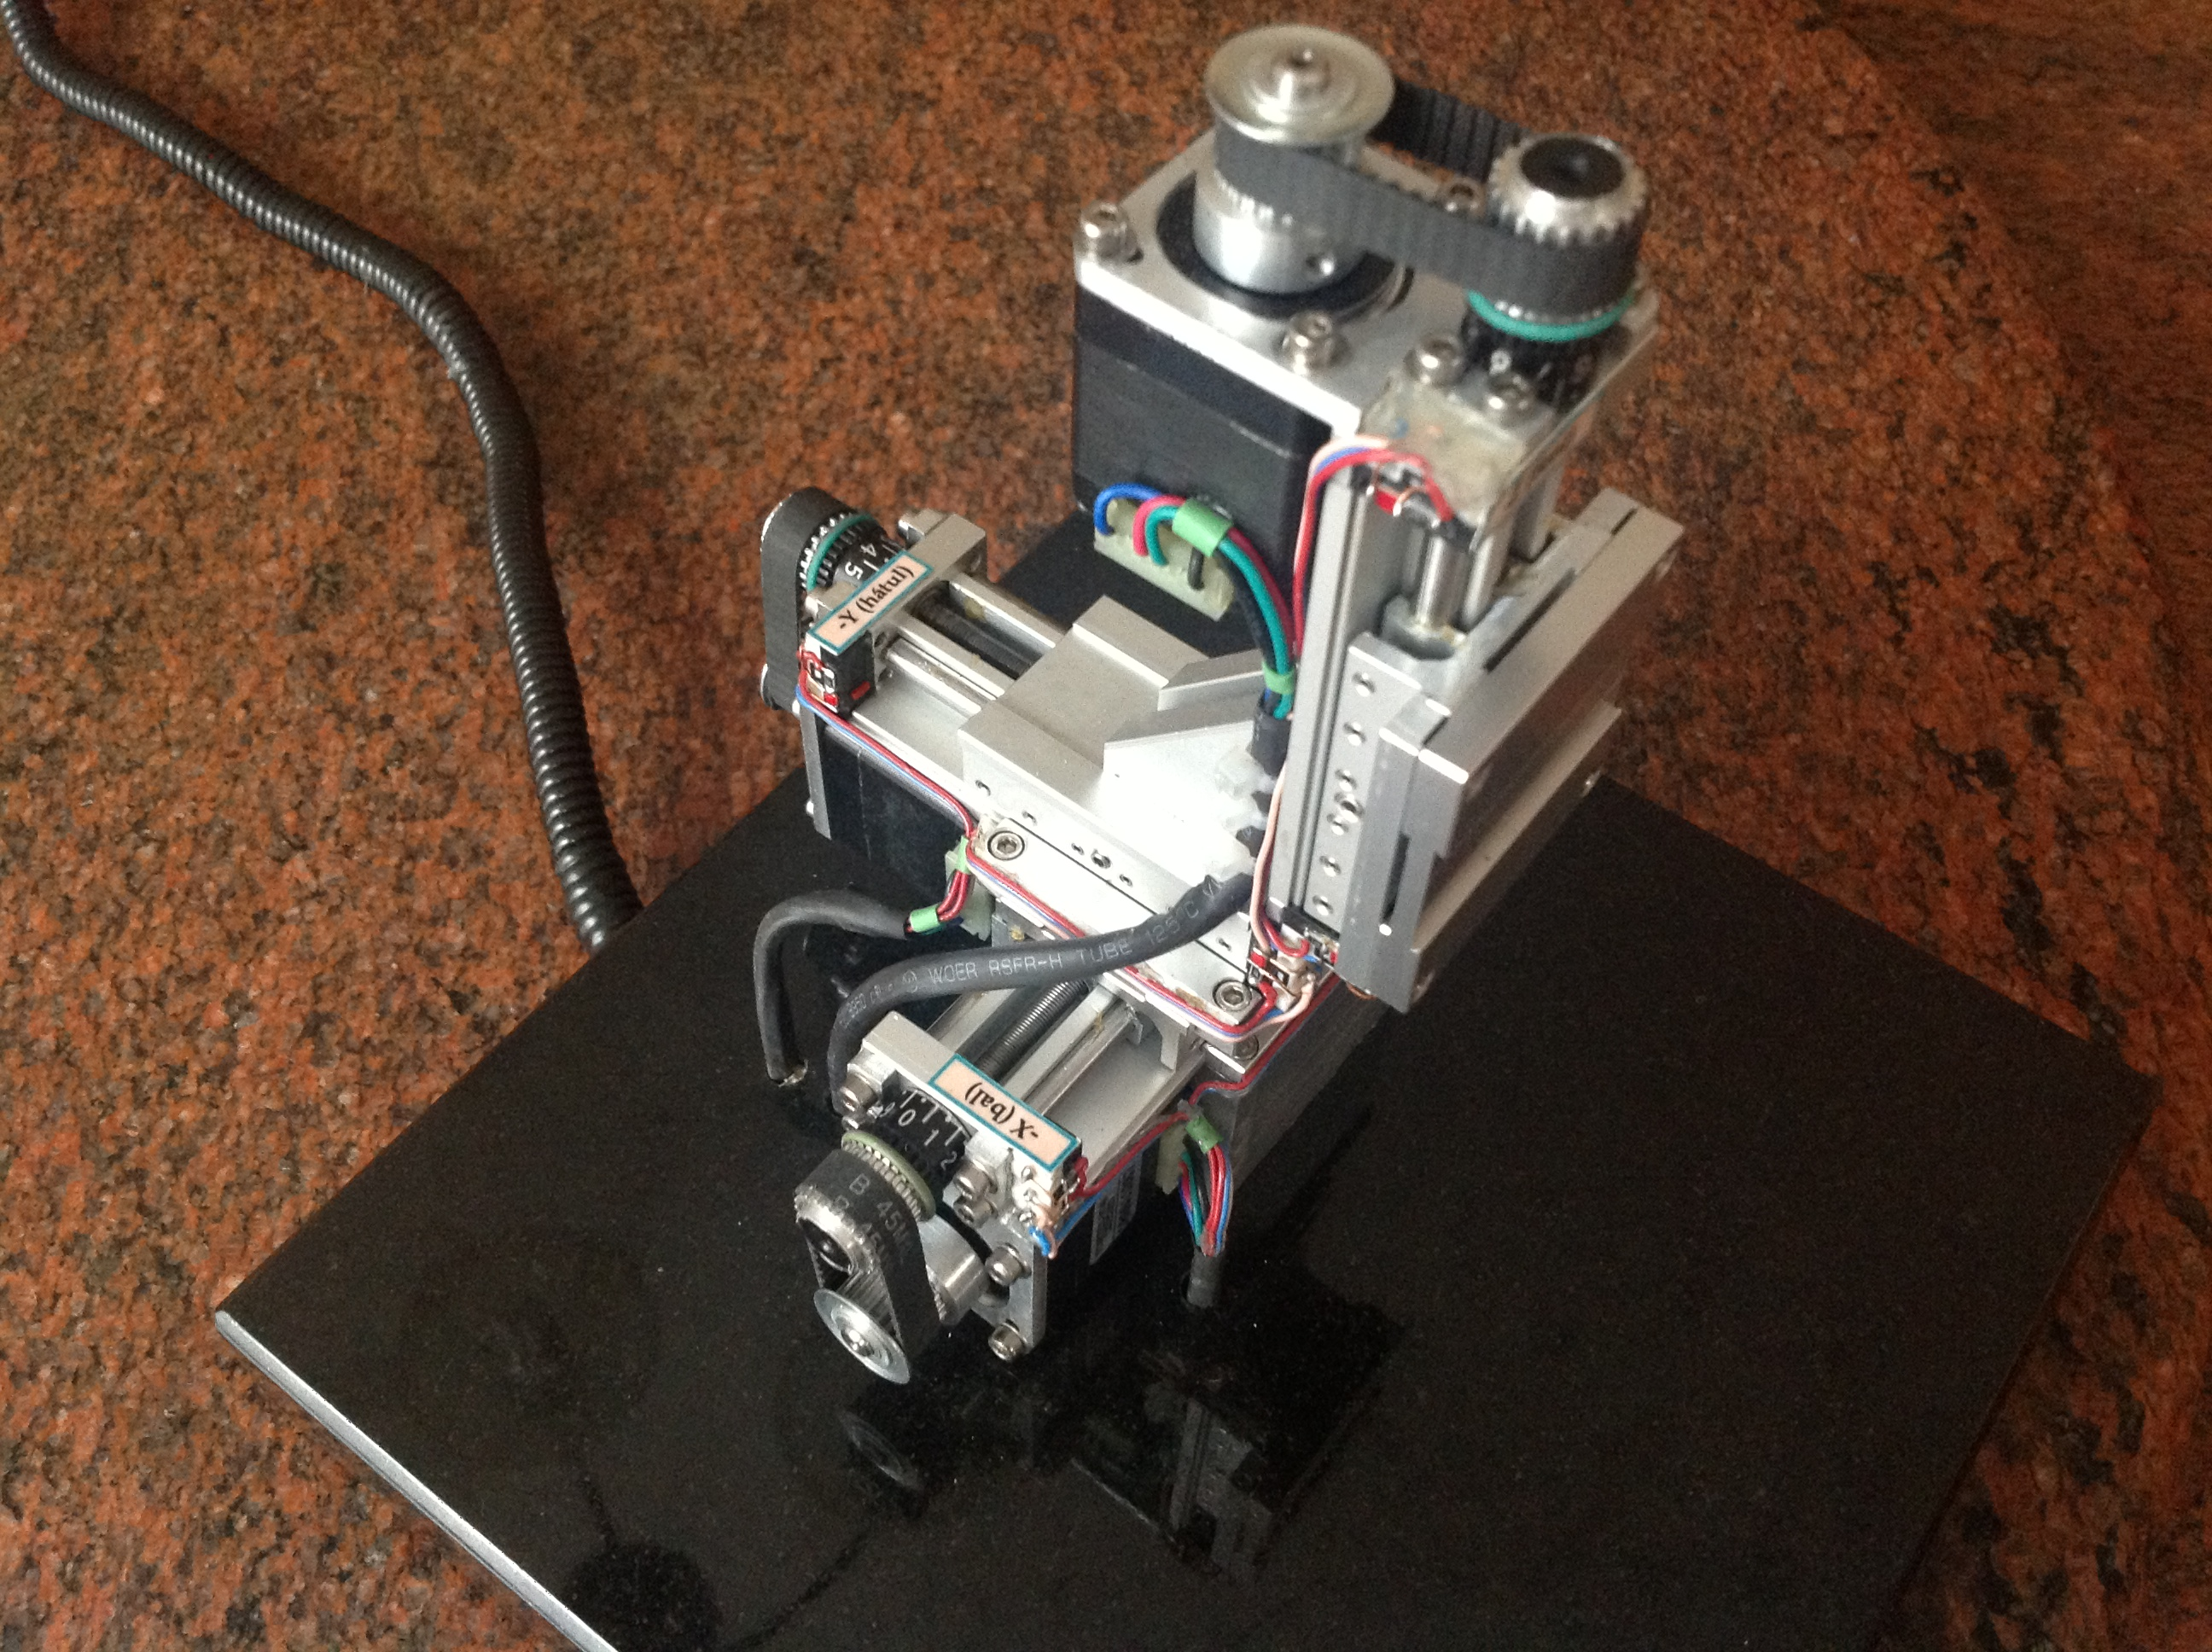
\includegraphics[width=0.3\textwidth]{img/agricom.jpg}\includegraphics[width=0.3\textwidth]{img/newport.eps}
\caption[The Scanning Electrochemical Microscopes I used in my work.]{The Scanning Electrochemical Microscopes I used in my work.
(A) Sensolytics SECM, (B) home-made SECM using Newport slide units, (C) home-made SECM using Domiline slide units driven with Nema 17 stepper motors, and (D) low cost, home-made 1D SECM using a slide unit from a DVD burner, driven by a stepper motor taken from a 5.25" floppy drive.}
\label{fig:secms}
\end{figure}

		\subsection{Homemade SECM}
Two microscopes out of the three I used during my work are homemade.
The first one was built from 3 Newport M-MFN25PP linear stages equipped with UE166PP stepper motors. 
Controller and driver was home-made from parts available in the local electronics store.
The other SECM was built from Domiline 15 linear stages.
Stepper motors for these were 3 Nema 17.
Motors were coupled to the shafts by ribbed belts.
It was controlled by a SD4DX USB Controller (Peter Norberg Consulting, Inc. 117 South Clay Ave. Ferguson, MO, USA), and driven by a Gecko step-and-direction driver board (Geckodrive, Inc. 14662 Franklin Ave, Santa Ana, CA.).
The control software was written in Java. 
	\section{Measuring corrosion current between a galvanic couple}
Corrosion current can't be measured directly, since the measurement itself would alter the current.
However, it is possible to calculate it by measuring the voltage drop on the two sides of a variable resistor, which connects the Mg and Fe samples together (Fig. \ref{fig:corrosion_current}).
Plotting the voltage over the resistance (E/R) with respect to resistance, the ''y,, interception will be 1 / $i$ at $R=0$, after reciprocating, corrosion current is obtained.
Using Faraday's law of electrolysis, Mg$^{2+}$ ion flow rate from the Mg/Al sample was estimated.

\begin{figure}
\centering
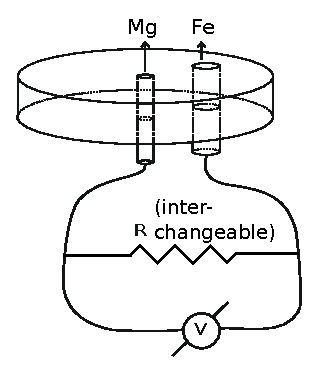
\includegraphics[width=0.3\textwidth]{img/corrosion_current.eps}
\caption[Circuit for measuring corrosion current between a galvanic couple.]{Circuit for measuring corrosion current between a galvanic couple.}

\label{fig:corrosion_current}
\end{figure}


	\section{Estimating ion-flux based on approaching curves}
To estimate the flux of Mg$^{2+}$ ions from the AZ63 sample, fixed height lateral scans and retracting scans were performed above the Mg sample, using solid contact Mg$^{2+}$ ISME electrode as measuring tip, and Ag/AgCl/3 M KCl reference with a homemade SECM.
Height of lateral scans was 100 $\upmu$m, resolution was 5 $\upmu$m, lateral distance was 5 mm with the Mg/Al sample in the centre.
Retracting curves were recorded at t = 10, 20, 30, 40, 50, 60 minutes after introduction of the corrosive media, step size was 5 $\upmu$m.
Since ionselective electrodes of this size have high resistance compared to the low input resistance of potentiometers, to avoid loading the potentiometric sensor, a homemade high impedance voltage follower circuit was used as current buffer based on the TL082 operational amplifier (Texas Instruments).
The potential was measured with a MeTeX potentiometer (MeTeX M-3630D) connected to a PC, the signal was recorded with the software provided by MeTeX.
Scans were performed with the galvanic pair both coupled, and uncoupled.
Corrosive media was distilled water saturated with air.
